\documentclass[11pt]{article}
\usepackage[utf8]{inputenc}
\DeclareUnicodeCharacter{2217}{*}
\DeclareUnicodeCharacter{2018}{'}
\DeclareUnicodeCharacter{2019}{'}
\DeclareUnicodeCharacter{201C}{"}
\DeclareUnicodeCharacter{201D}{"}
\DeclareUnicodeCharacter{2013}{--}
\DeclareUnicodeCharacter{2014}{---}
\DeclareUnicodeCharacter{2011}{-}
\DeclareUnicodeCharacter{2212}{-}
\DeclareUnicodeCharacter{2260}{$\neq$}
\DeclareUnicodeCharacter{2026}{\ldots{}}
\DeclareUnicodeCharacter{2192}{$\rightarrow$}
\usepackage{amsmath, amsthm, graphicx, latexsym, amsfonts, amsbsy, lscape, longtable, setspace, multirow, tabularx, booktabs, verbatim, bm, framed,etoolbox,xcolor,soul, comment, threeparttable, adjustbox, geometry, afterpage, changepage, float, ragged2e, geometry, siunitx,caption,subcaption}
\usepackage[longnamesfirst]{natbib}
\bibliographystyle{jpe}
% NOTE: need to use the following style to get rid of long citations (without et al.) after the first cite:
%\bibliographystyle{apacite}
\bibpunct{(}{)}{;}{a}{}{}
\linespread{1.5}
\newtheorem{prop}{Proposition}
\newtheorem{cor}{Corollary}
\newtheorem{assumption}{Assumption}
\colorlet{shadecolor}{gray!15}
\newenvironment{point}
  {\begin{shaded}}
  {\end{shaded}}

% LOAD CAPTION PACKAGE
\captionsetup{labelfont=bf}

% LOAD SUBFIGURE PACKAGE
%\usepackage{subfigure}
\usepackage{subcaption}
\renewcommand\thesubfigure{\alph{subfigure}}
\captionsetup[subfigure]{labelformat=parens}

% Hyperlink colors
\usepackage{color}
\usepackage{color}
\definecolor{myr}{rgb}{0.6,0,0}
\definecolor{myb}{rgb}{0,0,0.6}
\definecolor{myg}{rgb}{0,0.4,0}

\usepackage{hyperref}
\hypersetup{colorlinks,
    citecolor=myb,
    filecolor=myb,
    linkcolor=myr,
     urlcolor=myg}

% DEFINE FIGURE INSERT, CAPTION, AND NOTE COMMANDS
\newlength{\figwidth}
\newcommand{\figinpt}[2]{
    \settowidth{\figwidth}{\includegraphics[#1]{#2}}
    \setcaptionwidth{\figwidth}
    \centering
    \includegraphics[#1]{#2}}

\newcommand{\figcapt}[2][\linewidth]{
    \setcaptionwidth{#1}
    \centering
    \caption{#2}}

\DeclareTextFontCommand{\fignotefont}{\normalfont\footnotesize}
\newcommand{\fignote}[2][\linewidth]{
    \begin{minipage}[]{#1}
        \vspace{12pt}
        \fignotefont{#2}
    \end{minipage}}

\DeclareTextFontCommand{\tabnotefont}{\normalfont\footnotesize}
\newcommand{\tabnote}[2][\linewidth]{
    \begin{minipage}[]{#1}
        \vspace{12pt}
        \tabnotefont{#2}
    \end{minipage}}

% ADJUST PAGE MARGINS
\oddsidemargin 0in
\evensidemargin 0in
\textwidth 6.25in
\textheight 8.5in
\topmargin -.5in
%U.S. Auto Production: A structural analysis of contemporary automotive policies
\title{\textbf{Tariffs, Global Value Chains, and the Incidence of Protection: Evidence from US Automobiles}\vspace{20pt}}
\vspace{20pt} \author{\normalsize Luke Heeney,$^{1}$ Christopher R. Knittel,$^{1,2, 3}$ Jasdeep Mandia$^{1}$ \thanks{∗We are grateful for helpful comments and suggestions from the participants at the MIT CEEPR Seminar 2025, Association for Public Policy Analysis and Management (APPAM) Conference 2025.
\newline
 \newline \noindent $^1$ Center for Energy and Environmental Policy Research (MIT). $^2$ Sloan School of Management and MIT Climate Policy Center, Massachusetts Institute of Technology. $^3$ National Bureau of Economic Research.}}

\begin{document}
%\date{\medskip{} January 2026}
\date{\medskip{} April 23, 2026}
\maketitle

\begin{abstract}

%KNITTEL ALTERNATIVES
\footnotesize
\singlespacing
\setstretch{0.9}

\noindent
%How does protection affect prices, profits, and welfare in markets where firms possess market power and rely on global value chains for intermediate inputs? This paper studies how exposure to imported intermediate inputs shapes the incidence and welfare effects of tariffs in oligopolistic differentiated-product markets.

\noindent In many modern industries, firms compete in differentiated-product markets while relying on complex global value chains for intermediate inputs. In such settings, trade policies such as tariffs that affect final and intermediate goods operate not only through consumer substitution and firm pricing, but also through firms’ cost structures and sourcing decisions. This paper studies these dynamics in the U.S. automobile market. We develop a structural model of the U.S. automobile market that integrates random-coefficients demand, multiproduct firm pricing, and a flexible supply-side framework in which shocks to the cost of imported parts transmit imperfectly into manufacturers’ marginal costs. The model is disciplined by novel model-level data on imported-parts exposure and exploits exchange-rate variation to identify cost pass-through. Our counterfactual analysis quantifies the effects of alternative tariff policies on prices, profits, and welfare. First, tariffs on imported vehicles alone reallocate demand toward domestically assembled products and increase U.S. producer surplus, generating a gain of approximately \$1 billion for U.S.-headquartered firms, while reducing consumer surplus by about \$14 billion. Second, extending tariffs to imported intermediate inputs fundamentally alters these effects: consumer surplus losses roughly double, and producer surplus for U.S.-headquartered firms declines by about \$2.1 billion. Outcomes for U.S.-headquartered firms are highly heterogeneous: firms with greater exposure to imported parts experience losses, whereas those relying more on domestic inputs see an increase in profits. Overall, the results show that tariff incidence depends critically on firms’ exposure to global value chains and cannot be inferred from final assembly locations alone.
\bigskip
\\
\noindent \textit{Keywords:} tariffs, global value chains, differentiated products, automobile industry

\bigskip\noindent \textit{JEL:} L13, F13, L62
\end{abstract}

\newpage

\setcounter{page}{1}
%\onehalfspacing
%\setstretch{2}

\section{Introduction}\label{Section:sec_introduction}

%A central question in the analysis of trade and industrial policy is how protection affects prices, profits, and welfare in markets characterized by market power and globalized production
A central question in the analysis of trade and industrial policy is how protection affects prices, profits, and welfare in markets characterized by market power and globalized production \citep{bagwell1999economic}. In such settings, the incidence of protection depends on firms' exposure to foreign intermediate inputs and how tariffs pass-through to prices and costs \citep{goldberg1996goods,amiti2019tariff}.
In many modern industries, firms compete in differentiated-product markets while relying on complex global value chains for the intermediate inputs required to produce those goods \citep{antras2004global}. In such settings, policy instruments that target trade---including tariffs, subsidies, and domestic content requirements---operate not only through consumer substitution and firm pricing, but also through firms’ cost structures and sourcing decisions. As a result, the incidence of protection is not determined solely by the location of final assembly or the elasticity of demand, but depends critically on the exposure of domestic producers to foreign intermediate inputs \citep{amiti2019tariff,barrot2016input}.

This paper studies how intermediate-input exposure alters the incidence and welfare consequences of tariffs in oligopolistic differentiated-products markets. We show that when domestically assembled products rely heavily on imported inputs, policies seemingly intended to protect domestic producers can instead raise their marginal costs, weaken their competitive position, and reduce producer surplus.
More broadly, our analysis highlights that the distinction between ``domestic'' and ``foreign'' goods becomes blurred once production is fragmented across borders, and that ignoring global value chains can lead to misleading conclusions about the effects of trade policy.

We study these mechanisms in the context of the U.S.\ automobile market, a setting that is particularly well-suited to analyzing the importance of global production networks.
Almost half of the vehicles sold in the United States are assembled abroad, and of those assembled domestically, around half of the parts used are imported. Furthermore, the percentage of parts imported varies across models, ranging from roughly 25\% to over 90\% in 2024. Consequently, how tariffs on vehicles and automotive parts affect outcomes depends in part on heterogeneity in exposure to foreign parts imports across domestic firms, along with assembly location decisions and firms' pricing power.

To quantify these effects, we develop a structural model of the U.S.\ automobile market that integrates differentiated-products demand with firm pricing and global input sourcing. On the demand side, we estimate a random-coefficients discrete-choice model that captures realistic substitution patterns across hundreds of vehicle models and allows for rich heterogeneity in consumer price sensitivity and preferences for vehicle attributes \citep{nevo_measuring_2001,berry_automobile_1995,grieco_evolution_2024}.

On the supply side, we depart from the common assumption that the marginal costs of domestically assembled products are insulated from shocks to foreign input prices. Instead, we allow changes in the cost of imported automotive parts---driven by tariffs or exchange-rate movements---to transmit imperfectly into manufacturers’ marginal costs. Rather than modeling the high-dimensional sourcing problem directly, we discipline the relevant cost channel by estimating the reduced-form pass-through of changes in the cost of foreign parts to changes in marginal cost. This pass-through (cost shocks to marginal cost) parameter serves as a sufficient statistic for the combined effect of upstream cost absorption by suppliers, medium-run adjustments in firms’ sourcing decisions, and the share of marginal cost owing to parts. Exchange-rate variation provides the identifying variation for this channel, allowing us to capture how global cost shocks propagate to domestically assembled vehicles, while accounting for endogenous changes in sourcing decisions without requiring a fully specified model of parts sourcing.

Our analysis focuses on the medium run: we hold product offerings and assembly locations fixed while explicitly allowing firms to adjust prices and quantities in response to policy-induced cost changes, and accounting for potential endogenous changes in parts sourcing via our reduced-form sufficient statistic. This horizon is particularly relevant in industries such as automobiles, where model lineups and production locations are determined years in advance, but pricing and input sourcing exhibit greater medium-run flexibility\footnote{News reporting indicates medium-term flexibility in where automakers source certain parts from. See, for example, this \href{https://www.reuters.com/business/autos-transportation/how-cheap-component-could-help-kill-off-combustion-cars-2022-05-30/}{2022} article from Reuters.}.
Our counterfactuals are well-suited to evaluating the effects of trade policies before potential changes in production location occur.

We estimate the model using a novel model-year level dataset for the U.S. light-duty automobile market covering 2015–2024. The dataset combines sales, vehicle characteristics, and manufacturing data (assembly location and vehicle foreign content) from sources such as S\&P Polk, DataOne, and the National Highway Traffic Safety Administration (NHTSA), and is supplemented with data on EV subsidies, consumer demographics, and exchange rates.

Our counterfactual analysis yields three core results. First, tariffs on imported final goods alone tend to reallocate demand toward domestically assembled products. While the price increase for domestically assembled vehicles is minimal, a 5.3 percentage point increase in market share raises the producer surplus of these firms by about \$1 billion.\footnote{The market share calculation includes the outside good share in the denominator.} In this case, domestic producers benefit from protection despite higher overall prices. Consumer surplus falls by \$14.1 billion, while tariff revenue rises by \$14.6 billion, resulting in a net US gain of \$1.5 billion. Second, extending tariffs to imported intermediate inputs reverses these producer gains. By raising marginal costs for domestic assemblers that rely on foreign parts, parts tariffs can erode or reverse the competitive gains from taxing imported final vehicles. This roughly doubles consumer welfare losses and reverses US producer surplus from a gain of \$1.0 billion to a loss of \$2.1 billion. However, these aggregate effects mask substantial heterogeneity among firms: while many U.S.-headquartered firms (e.g., Chevrolet, GMC, and Ford) experience losses due to their exposure to imported parts, firms with lower reliance on foreign inputs (e.g., Tesla, Jeep, Honda, and Toyota) are able to increase profits as their products benefit from lower marginal costs relative to competitors. In both scenarios, higher-income households account for a substantial share of consumer welfare losses, with the top quintile alone representing about 40\%. Third, reinstating EV subsidies generates sizable welfare gains. Consumer surplus increases by approximately \$10.1 billion, while U.S.-headquartered firms’ producer surplus rises by about \$1.8 billion. These gains are accompanied by an expansion in EV market share, total vehicle sales, and the number of vehicles assembled in the United States.

The paper contributes to several literatures in industrial organization and trade. First, we apply differentiated-products IO tools to evaluate trade policy in the automobile market while explicitly incorporating global value chains, extending analyses of the auto industry \citep{berry_automobile_1995, grieco_evolution_2024} by allowing policy to operate through imported intermediate inputs as well as through final-goods trade. A key ingredient is new, model-level data that links every vehicle model sold in the United States to the value share of its parts imported, including the primary foreign-sourcing country. This enables us to measure exposure to trade policy and foreign cost shocks at the level at which pricing and substitution occur.

Second, we introduce a flexible supply-side pass-through component that connects foreign cost shocks to vehicle marginal costs. We estimate how marginal costs respond to shocks as a function of a model’s imported-parts exposure.

Third, we quantify the medium-run incidence of alternative tariff designs, distinguishing between tariffs applied only to imported vehicles and tariffs applied to both imported vehicles and imported parts. In doing so, we complement recent quantitative work on automobile tariffs and subsidies \citep{grieco_evolution_2024, allcott_effects_2024} by emphasizing transmission through firms’ exposure to input sourcing rather than through changes in conduct or long-run capacity adjustments.

Our analysis is most closely related to independent and concurrent work on firm conduct and scale economies in the automobile market \citep{duarte_conduct_2025}. That paper uses a demand system with preferences calibrated to 2018 \citep{grieco_evolution_2024}. Our approach differs along three key dimensions. First, we capture upstream absorption and sourcing adjustments through an estimated pass-through sufficient statistic. Second, we study the current market environment using data from 2015 to 2024, estimating contemporary consumer preferences and the prevailing vehicle choice set. This is important in a rapidly evolving market: between 2015 and 2024, the SUV share increased from 31\% to 50\%, while EV adoption rose from less than 0.5\% to 7.3\%. Accounting for these shifts in demand and product availability is quantitatively important. Third, we incorporate a more precise representation of the current tariff regime by allowing tariffs to vary across countries rather than imposing a uniform rate.

Our findings speak to the incidence of trade policy in the presence of firm heterogeneity and fragmented production. The downstream effects of tariffs on consumers and domestic producers depend on market structure and input exposure. By embedding global sourcing within a differentiated-products equilibrium framework, we show that policies that appear protective when focusing on final goods trade can impose substantial costs when intermediate inputs are taken into account. While our empirical analysis focuses on automobiles, the mechanisms we document are likely to operate in other industries with global value chains, such as electronics, machinery, and clean energy technologies, where recent trade policies have targeted both final goods and key intermediate inputs.

The remainder of the paper proceeds as follows. Section~\ref{sec:sec_data} describes the data. %, including novel information on model-level parts sourcing.
Section~\ref{sec:sec_model} presents the demand model and supply-side framework. Section~\ref{sec:sec_estm} describes the estimation procedure, and section~\ref{sec:sec_results} discusses the results. Section~\ref{sec:sec_counterfactuals} reports counterfactual tariff simulations and welfare implications. Section~\ref{sec:sec_conclusion} concludes.



\section{Data and descriptive statistics}\label{sec:sec_data}

\subsection{Data}
We construct a novel model-year level dataset for the U.S. light-duty automobile market covering 2015–2024 by combining sales, vehicle characteristics, and manufacturing data. Our primary sources are sales data from S\&P Polk, vehicle characteristics from DataOne, and manufacturing data—including assembly location and foreign content—from the National Highway Traffic Safety Administration (NHTSA). We also incorporate data on EV subsidies, consumer demographics, and exchange rates. This section describes each data source and outlines the procedures used to construct the dataset.

%old We construct a vehicle dataset for 2015–2024 at the model-year level by matching sales, vehicle characteristics, and manufacturing data of the US light-duty automobile market. Our primary data sources are sales data from S\&P Polk, vehicle characteristics from DataOne, and manufacturing data  (assembly location and vehicle foreign content) from the National Highway Traffic Safety Administration (NHTSA). We also use data on EV subsidies, consumer demographics, and exchange rates. This section describes each data source in detail and explains the dataset construction and the matching procedures used.

\paragraph{Vehicle Sales Data}
S\&P Polk provides annual data on automotive registrations for 2015--2024. The dataset reports, for each year, the total number of registered vehicles by trim (and model year) at the ZIP-code level. We construct a proxy for new sales by computing the year-over-year change in registrations within each ZIP code, restricting attention to vehicles whose model year matches the calendar year. This restriction helps limit spurious ``sales'' driven by households re-registering an existing vehicle after moving to a different ZIP code. However, it likely understates true new-vehicle sales because new purchases may include vehicles from prior model years.\footnote{For example, we observe 11.27 million vehicle sales for 2024, while reported new-vehicle sales were 15.85 million (\cite{wardsauto_most_2025}).}

We define products at the model-year level and aggregate trim-level sales to the model level by summing sales across all trims associated with a given model. We aggregate zip-code-level data across the US. To convert sales into market shares, we define the market size as the number of US households in a given year divided by 6, reflecting an average vehicle replacement cycle of six years, following \cite{cosar_what_2018} and \cite{allcott_effects_2024}.\footnote{We also test using a denominator of 2.5, as suggested by \cite{grieco_evolution_2024} and \cite{sabal_product_2025}, and allowing for a random coefficient on mean utility for the inside good. The results are qualitatively similar.}

\paragraph{Vehicle Characteristics Data}
Vehicle characteristic data are obtained from DataOne, which provides trim-level information on a wide range of attributes, including price, horsepower, weight, length, engine type, and assembly location. We convert these trim-level data to the model level by taking the median of each characteristic across all trims within a given model.

\paragraph{Manufacturing: Assembly Location and Vehicle Foreign Content Data}
The American Automotive Labeling Act (AALA), implemented under Part 583 of the US Code of Federal Regulations, requires manufacturers of consumer vehicles sold in the United States to report, among other information, the vehicle’s assembly location and the share of parts content (by value) originating from the United States and Canada jointly (henceforth "domestic") and from each foreign country from which imported parts exceeds 15\% of total parts value.\footnote{The data do not distinguish between US and Canadian parts.} We obtain these data for 2015--2024 from the National Highway Traffic Safety Administration (NHTSA), which compiles manufacturers’ reports on assembly locations and parts origins. These data are available for free on the NHTSA website.

Because reporting is subject to the 15\% threshold, we do not observe the full set of foreign-sourced parts: depending on the year, the source country is unreported for between 18\% (2016) and 26\% (2024) of parts value. The AALA data also have incomplete coverage across models, requiring us to impute missing values for domestic and foreign parts shares.\footnote{One firm, Rivian, does not appear in the data at all.} When a firm or model is missing observations for a subset of years, we impute in three steps. First, if the model is observed in adjacent year(s), we assign the closest available value (or the average of the nearest observations on either side). Second, if the model is never observed, we use the make-level average domestic parts share, using the closest year(s) in which that make-level average is available. Finally, if a make is entirely unobserved, we assign the overall average domestic parts share among U.S.-assembled vehicles (this occurs only for Rivian).

\paragraph{Electric Vehicle Subsidy Data}
Federal EV purchase incentives in the United States changed substantially over the study period. The long‑standing Section 30D federal tax credit, which provided up to \$7{,}500 for eligible new plug‑in vehicles, featured manufacturer‑specific phase‑outs once cumulative US sales exceeded 200{,}000 units. The Inflation Reduction Act (IRA), enacted in August 2022, restructured the program by conditioning eligibility on final assembly in North America and, beginning in 2023, on additional sourcing requirements. Vehicles acquired after September 30, 2025, are no longer eligible for the credit (\cite{internal_revenue_service_clean_2025}).

Additionally, beginning January 1, 2023, Section 45W credits of up to \$7,500 for light-duty electric vehicles were made available to businesses. Consumers were able to access this credit via the 'leasing loophole' that is explicitly modeled in \cite{allcott_effects_2024}.

We construct a vehicle‑level EV subsidy series using data from the US Department of Energy’s Tax Incentive Data Services (\cite{department_of_energy_tax_2025}). For each product, we assign the pre‑2023 statutory credit for model years up to 2022, a date‑weighted average of pre‑ and post‑2023 credits for model year 2023 (reflecting the mid‑April implementation of the new rules), and the post‑2023 credit for model year 2024. We then apply the statutory manufacturer phase‑out schedules during the 2019–2022 period and implement the IRA assembly eligibility rules. From 2023 onwards, all vehicles that were previously eligible for a Section 30D credit are assumed to receive the Section 45W credit in full.
% add_later
Appendix Table \ref{tab:avg_ev_subsidy_by_producer_45W} reports the average EV subsidy by manufacturer in each year.

%Federal EV purchase incentives in the US shifted sharply during the study period. The long‑standing Section 30D credit (up to \$7,500) applied to eligible new plug‑in vehicles, with manufacturer‑specific phase‑outs after 200,000 cumulative US sales (notably affecting Tesla and Ford). The Inflation Reduction Act, enacted in August 2022, restructured eligibility by tying credits to North American final assembly and, beginning in 2023, to additional sourcing criteria. Vehicles acquired after September 30, 2025, are no longer eligible for incentives (\cite{internal_revenue_service_clean_2025}). We constructed the EV subsidy series by extracting vehicle‑level federal tax credit amounts from the US Department of Energy “Tax Incentive Data Services” (\cite{department_of_energy_tax_2025}). For each product, we set the applicable credit as the pre‑2023 value for model years $\leq$ 2022, a date‑weighted average of early‑ and post‑2023 credits for model year 2023 (reflecting the mid‑April rule change), and the post‑2023 value for 2024. We then applied the statutory manufacturer phase‑out factors for Tesla and Ford in the 2019–2022 period and implemented the assembly eligibility adjustment consistent with the Inflation Reduction Act: non‑US assembly yields zero credit from 2023 onward, while 2022 credits are pro-rated by the fraction of the year before the Aug. 15, 2022 assembly requirement. Appendix Table \ref{tab:avg_ev_subsidy_by_producer} presents the average subsidy available for EVs from a given manufacturer.

\paragraph{Consumer Demographic Data}
To incorporate geographic heterogeneity while keeping the model computationally tractable, we aggregate the nine US Census divisions into six regions. Appendix Figure \ref{fig:div_map} maps our modified divisions and the states included in each.

We obtain household demographic data from \cite{ruggles_ipums_2025}, including the number of households (nationally and by division-year), household income, and household location. We use these data to construct the demographic moments described later.

%We consolidate the nine US Census divisions into six. This choice is made to reduce the computational burden of simulating sufficient agents from all nine divisions. Appendix Figure \ref{fig:div_map} shows the states included in our modified divisions. We collect US household demographic data from \cite{ruggles_ipums_2025}, including the number of total households in the US (and in each division) in each year, household incomes, and household location. We utilize this data to construct moments, explained later.

\paragraph{Vehicle Data Matching}
We merge the three datasets (sales, vehicle characteristics, and manufacturing) by model name and model year. To match, we use a combination of formulaic and manual matching, achieving coverage of at least 97\% of annual sales in every year of the sample. Sales prices are deflated to constant 2015 US dollars. This gives us year-model level data on sales, median vehicle characteristics, and manufacturing.

%\subsection{Summary Statistics}

\subsection{Descriptive Statistics}

\paragraph{Sales by Vehicle Type and Assembly Location}
\begin{figure}[!htbp]
\centering
\begin{subfigure}[t]{0.48\linewidth}
    \centering
    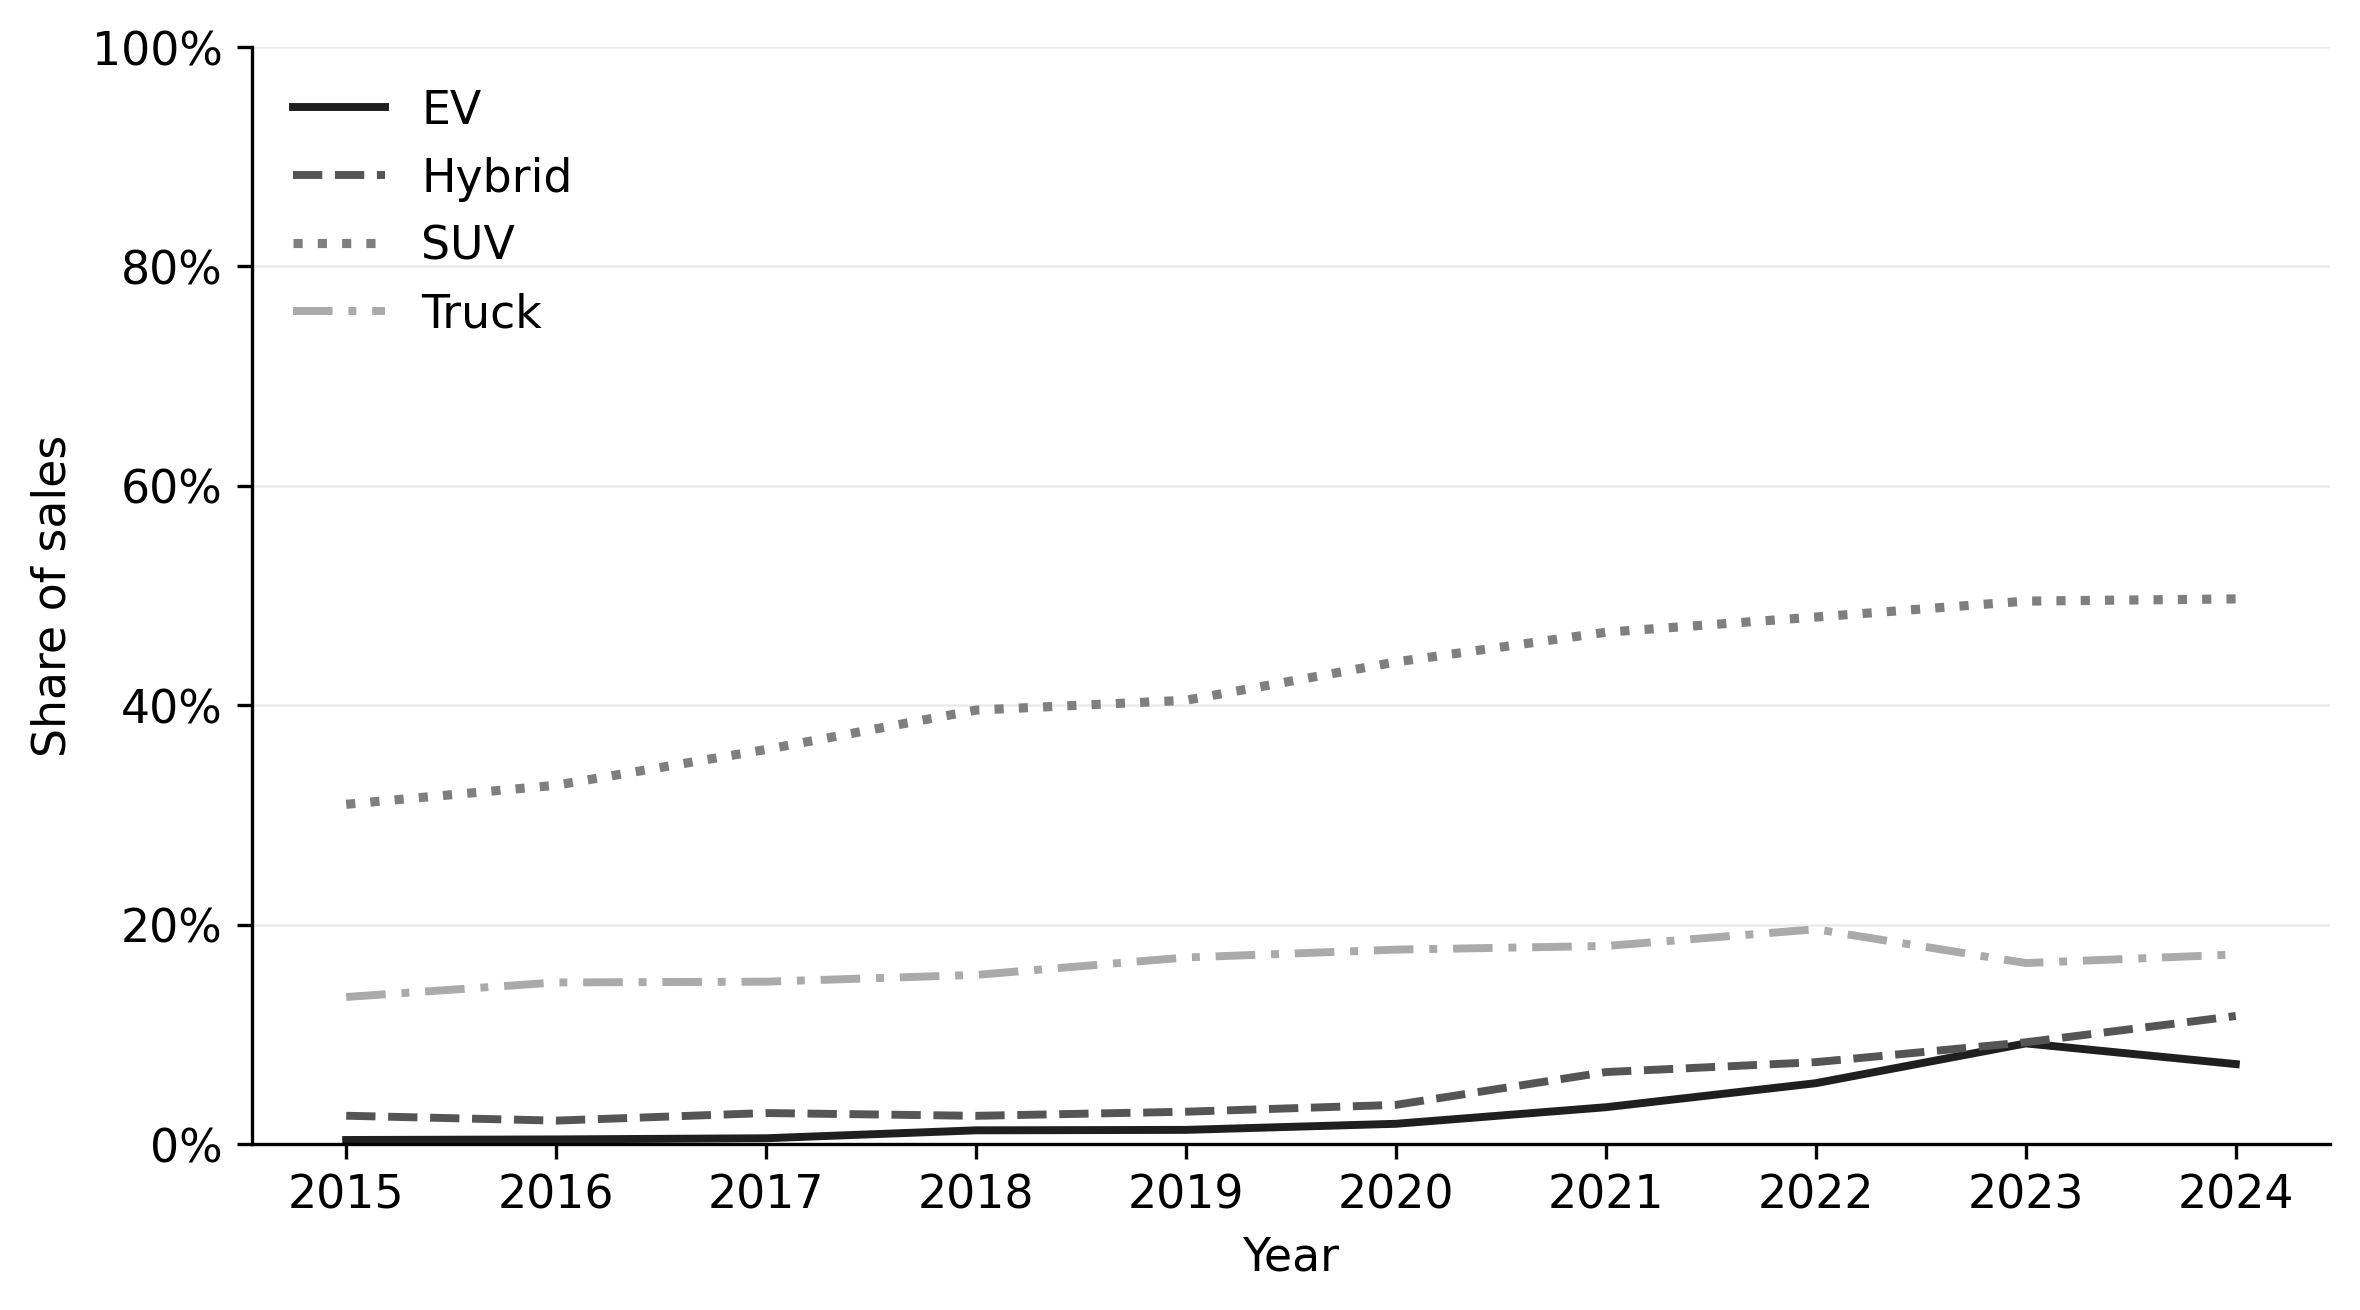
\includegraphics[width=\linewidth]{generated/graphs/trends1.png}
    \caption{Trends in sales by vehicle type}
    \label{fig:trends}
\end{subfigure}\hfill%
\begin{subfigure}[t]{0.48\linewidth}
    \centering
    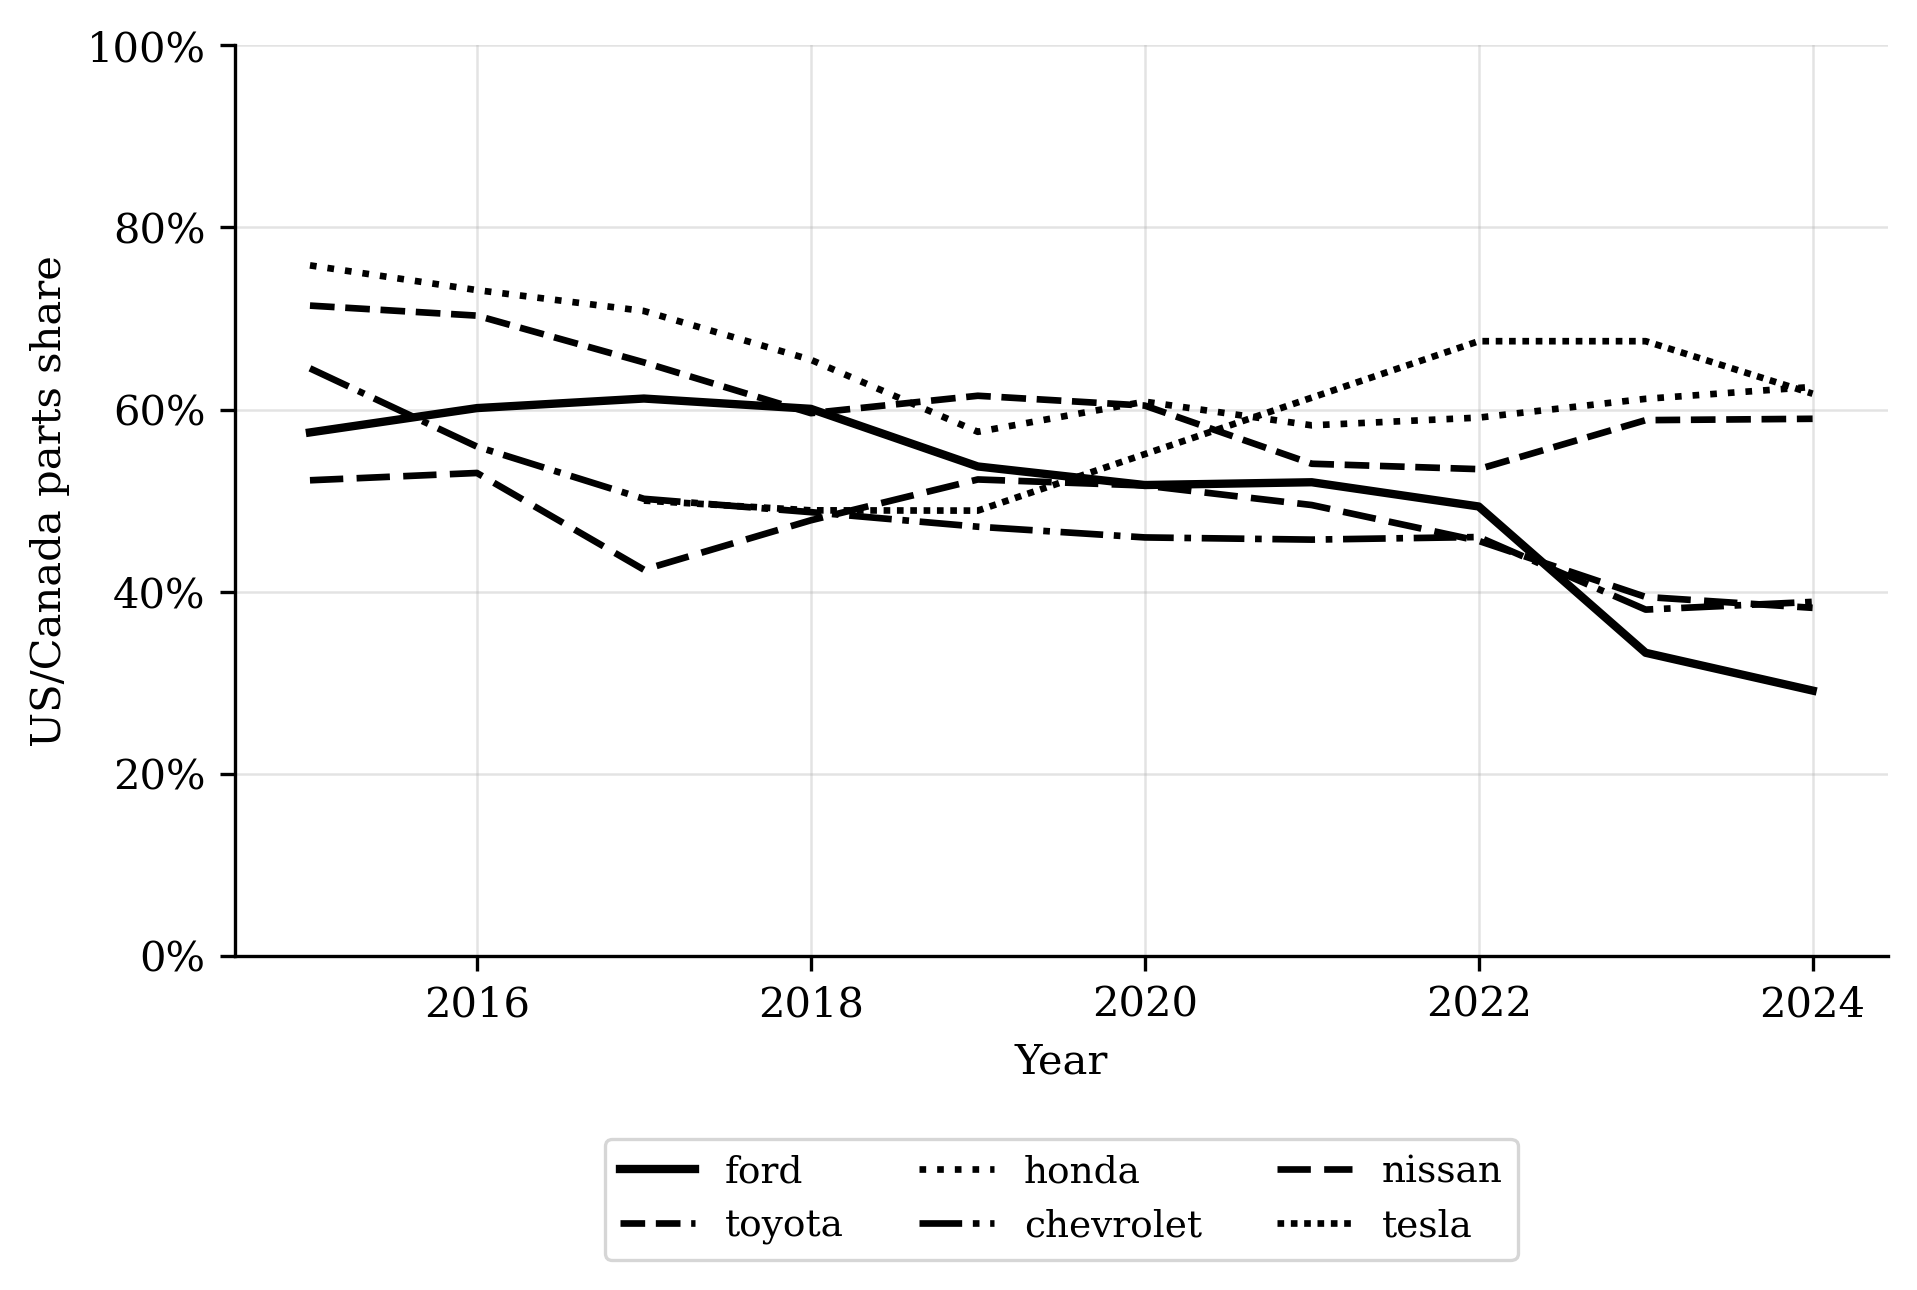
\includegraphics[width=\linewidth]{generated/graphs/domestic_share.png}
    \caption{Share of domestic content in domestically assembled vehicles (by value)}
    \label{fig:dom_share}
\end{subfigure}
\caption{Trends: sales by vehicle type and share of domestic content}
\label{fig:trends_and_domestic_content}
\begin{flushleft}
\footnotesize
\textit{Notes:} Panel (a) shows the evolution of vehicle sales by type over time. Panel (b) reports the average share of domestic (U.S. and Canadian) content in vehicles assembled in the United States, measured by value. The figures highlight shifts in demand composition and changes in the sourcing of intermediate inputs over the sample period.
\end{flushleft}
\end{figure}

Figure \ref{fig:trends} plots the evolution of sales shares by vehicle type from 2015 to 2024. Two notable shifts occur over the sample period. First, electric vehicles (EVs) expand rapidly: in 2015, they account for a negligible share---less than 0.5\% of purchases---rising to 7.3\% by 2024. Second, SUVs become substantially more prevalent, increasing from 31\% of sales in 2015 to 50\% in 2024. Truck sales also gain share over this period, though the increase is more modest.

Roughly half of vehicles purchased in the United States are assembled domestically. Among imported vehicles, Figure \ref{fig:sales_sources} shows that in 2024, the largest source countries are Japan and Mexico. Over the sample period, Canada’s share declines substantially.

Appendix Table \ref{tab:summary_by_type} describes the matched data after the exclusion of vehicles priced above \$100,000 USD (in 2015 dollars) and vehicles with market share below 0.001\% \footnote{This trimming amounts to a loss of less than 1\% of the total market share of inside goods in any given year.}. Over the sample period, 75\% of cars are imported, while only 8\% of trucks are foreign-assembled.

\paragraph{Foreign Content}
For vehicles assembled in the United States, the share of parts value sourced from the United States and Canada declines over the sample period, though the pace of decline varies substantially across firms. Figure \ref{fig:dom_share} plots trends in the domestic (U.S. and Canadian) parts share for the five largest US automakers—defined by sales of domestically assembled vehicles—along with Tesla, which we include to represent the EV segment.

By 2024, the firms shown in Figure~\ref{fig:dom_share} display a pronounced bimodal distribution in domestic parts sourcing. This pattern reflects persistent differences in firms' production architectures and supply-chain configurations, which generate substantial heterogeneity in exposure to foreign input cost shocks. We exploit this cross-firm and time-series variation in input exposure to identify how changes in the cost of imported parts are transmitted into product-level marginal costs. This variation provides the key empirical leverage for isolating the cost channel through which global value chains mediate the incidence of trade policy.

%In addition to the percentage of US and Canadian (henceforth 'domestic') parts, manufacturers are required to report the source and percentage of imported content from any country where the value of the parts sourced from that country exceeds 15\% of the total parts value. Of the observed sources of foreign parts, Japan and Mexico are by far the largest. Figure \ref{fig:sources} shows how this share has shifted over the course of our sample. We do not observe all foreign-sourced parts in the data; across the years in our data the source location of between 17.4\% (2016) and 26.5\% (2024) of parts by value are unobserved.  Finally, the data has imperfect coverage across models, so we must impute some values for the percent of parts sourced from domestic/foreign sources.\footnote{One firm, Rivian, does not appear in the data at all.} Some firms or models are missing observations for a subset of years. In these cases we impute values according to the following steps: first, if there is an observation for a given model in (a) neighboring year(s), we take the value (average) for that model from the closest available observation(s); second, if there is no available model observation, we take the average value for domestic parts percentage for vehicles of the same make, and if necessary fall back to the closest year(s) where this average is available; finally, if there are no observations for a given make we allocate the average domestic content percentage of all US vehicles (this only occurs in the case of Rivian).

Among the reported foreign sources, Japan and Mexico account for the largest shares. Appendix figure \ref{fig:sources} shows how the composition of reported foreign content evolves over our sample period.

\section{Model}\label{sec:sec_model}
\subsection{Demand}
We model US consumer demand for vehicles using a random-coefficients discrete choice framework following \cite{berry_automobile_1995} (BLP). A key advantage of this approach is that it allows consumers to have heterogeneous preferences over vehicle attributes---such as price, size, performance, and powertrain type (e.g., EV vs.\ ICE)---which generates flexible substitution patterns across products and heterogeneous willingness-to-pay. We estimate the demand-side parameters using observed market shares (and additional demographic moments described below) and match them to the shares implied by the model.

\subsubsection{Consumer Choices and Market Shares}

In each year \(t\), consumer \(i \in \mathcal{I}\) chooses among products \(j \in \mathcal{J}_t\) and purchases the product that delivers the highest utility. Consumers may also choose the \emph{outside good}—that is, make no vehicle purchase in year \(t\)—which we normalize to have utility zero and include in \(\mathcal{J}_t\) with index \(j=0\).

We model consumer‑specific utility as follows. In each market (year) \(t\), consumer \(i\) derives utility from vehicle \(j\) given by:
\begin{equation}\label{eq:BLP_util}
    u_{ijt} = \phi_{it} + \beta_{i}' \mathbf{X}_{jt} + \alpha_{it}\bigl(p_{jt} - \tau_{jt}\bigr) + \xi_{jt} + \varepsilon_{ijt},
\end{equation}
where \(\phi_{it}\), \(\boldsymbol{\beta}_{i}\), and \(\alpha_{it}\) denote consumer‑specific preferences for the inside good, observed product characteristics \(\mathbf{X}_{jt}\), and price, respectively. The price faced by the consumer is the manufacturer’s suggested retail price (MSRP) \(p_{jt}\), set by the firm, net of any applicable subsidy for electric or hybrid vehicles \(\tau_{jt}\).\footnote{Following \cite{allcott_effects_2024}, we assume that each EV transaction reflects the full \$7,500 federal tax credit. This abstracts from income-based eligibility constraints as well as domestic content requirements that may bind for direct purchases but not for leases (the so-called ``leasing loophole''). This assumption is consistent with modeling the price faced by a marginal consumer who is leasing a vehicle. We also note that our identification strategy instruments for price using exchange rate movements, so any discrepancy between statutory and realized subsidies does not affect our estimates, provided it is orthogonal to the instrument.} The term \(\xi_{jt}\) captures an unobserved product‑year utility shock common across consumers, and \(\varepsilon_{ijt}\) is an idiosyncratic consumer–product‑specific utility shock assumed to follow a Type I extreme value distribution.

The vector of observed characteristics \(\mathbf{X}_{jt}\) includes horsepower, vehicle footprint, miles per gallon, indicators for vehicle type (car, truck, SUV, van), and powertrain type (ICE, EV, hybrid), as well as brand fixed effects and indicators for luxury and European brands. We also include interactions between year and EV, SUV, and hybrid indicators to capture evolving consumer preferences for these vehicle types, as well as time‑varying quality changes—particularly for EVs and hybrids—arising from factors not fully captured by observed characteristics, such as improvements in charging infrastructure.

To capture heterogeneity in consumer tastes, we allow both observed demographics and unobserved preference heterogeneity to affect preferences for vehicle characteristics. Specifically:
\begin{align}
    \phi_{it} &= \bar{\phi}_t + \phi \cdot \log(\text{income}_i), \\
    \beta_{ik} &= \bar{\beta}_k + \sigma_k \nu_{ik} + \sum_d \pi_{kd} \mathbf{1}\{D_i = d\}, \\
    \alpha_{it} &= \bar{\alpha} + \alpha \cdot \log(\text{income}_i),
\end{align}
where \(\nu_{ik}\) captures unobserved taste heterogeneity, \(D_i\) denotes consumer demographic group membership, and \(k\) indexes vehicle characteristics. The terms \(\nu_{ik}\) are i.i.d.\ consumer‑specific taste shocks drawn from a standard normal distribution. The variable \(D_i\) denotes the U.S.\ regional division in which consumer \(i\) resides, and \(\mathcal{T}\) denotes the subset of characteristics for which we allow region‑specific preference shifters (SUV, truck, and EV indicators). Not all characteristics are permitted to exhibit unobserved heterogeneity or demographic interactions; for characteristics without such variation, the corresponding parameters \(\sigma_k\) and/or \(\pi_{kd}\) are set to zero.\footnote{We divide the United States into six regional divisions: Northeast, North Central, South Pacific, South Central, Mountain, and Pacific.}

\cite{berry_automobile_1995} shows that, under the Type I extreme value assumption on \(\varepsilon_{ijt}\), market shares are obtained by integrating the individual‑level logit choice probabilities over the distribution of consumer heterogeneity. Accordingly, the market share of product \(j\) in market \(t\) is given by:
\begin{align}\label{eq:blpshares}
    s_{jt} = \int
    \frac{\exp\!\left(\phi_{it} + \beta_{i}'\mathbf{X}_{jt} + \alpha_{it}(p_{jt} - \tau_{jt}) + \xi_{jt}\right)}
    {1 + \sum_{k \in \mathcal{J}_t \setminus \{0\}}
    \exp\!\left(\phi_{it} + \beta_{i}'\mathbf{X}_{kt} + \alpha_{it}(p_{kt} - \tau_{kt}) + \xi_{kt}\right)}
    \, dF(i),
\end{align}
\noindent where \(F(i)\) denotes the joint distribution of consumer‑specific attributes.

\subsubsection{Firm Pricing and Marginal Costs}
Under the assumption of static Nash-Bertrand pricing, the estimated demand system allows us to recover product-level marginal costs and markups, following \cite{berry_automobile_1995}.

Equation \eqref{eq:blpshares} expresses market shares \(s_t(\mathbf{p}_t)\) as a function of the vector of prices set by firms in market \(t\). Let \(s_t(\mathbf{p}_t)\) denote the \(J_t \times 1\) vector of product market shares, and let \(\frac{\partial s_t}{\partial \mathbf{p}_t'}\) denote the \(J_t \times J_t\) Jacobian matrix of shares with respect to prices. This Jacobian is computed from the random-coefficients demand system and integrated over consumer heterogeneity. Firms are assumed to jointly maximize profits across all products in their portfolios.

We define the ownership matrix \(\Omega_t\) as:
\[
(\Omega_t)_{jk} =
\begin{cases}
1 & \text{if products } j \text{ and } k \text{ are owned by the same firm in market } t, \\
0 & \text{otherwise.}
\end{cases}
\]

For each market \(t\), the first-order condition for profit maximization is
\begin{align}\label{eq:blp_mc}
    s_t(\mathbf{p}_t)
    \;+\;
    \left[\Omega_t \odot \frac{\partial s_t(\mathbf{p}_t)}{\partial \mathbf{p}_t'}\right]
    (\mathbf{p}_t - \mathbf{c}_t)
    \;=\; \mathbf{0},
\end{align}
where \(\odot\) denotes the element-wise (Hadamard) product, and \(s_t\), \(\mathbf{p}_t\), and \(\mathbf{c}_t\) are \(J_t\)-dimensional vectors of market shares, prices, and marginal costs, respectively.

In practice, the derivatives \(\partial s_t / \partial \mathbf{p}_t'\) are computed numerically using \texttt{PyBLP}, and marginal costs are recovered by inverting equation \eqref{eq:blp_mc}.

\subsection{Supply}
Having recovered product-level marginal costs from firms’ pricing behavior, we study how exposure to foreign intermediate inputs shapes the cost channel through which trade policy affects equilibrium outcomes. In markets with fragmented production, tariffs on intermediate inputs can raise the marginal costs of domestically assembled goods, altering firms’ competitive positions and the incidence of protection. Our objective in this section is to characterize how shocks to the cost of imported parts transmit into marginal costs for vehicles assembled in the United States, and how this transmission varies with firms’ reliance on foreign inputs.

Because we are interested in estimating the effect of US tariffs on vehicle costs, we design the supply-side analysis to identify how changes in the prices of foreign parts affect the marginal costs of vehicles assembled in the United States, allowing the effect to vary with each vehicle’s exposure to imported inputs. We model marginal costs only for domestically assembled vehicles. For these vehicles, we observe (i) the share of parts value sourced from the United States or Canada and (ii) the share of parts value imported from specific foreign countries when the value imported from a given country exceeds 15\% of total parts value.

In this section, we define a product \(j\) as a make–model pair observed over multiple years (e.g., \emph{Ford Bronco}), while allowing product characteristics to vary over time. This definition is required for our empirical specification and implies that we drop products that do not appear—or cannot be reliably matched—across multiple years.

Let \(\rho_{d,jt}\) denote the share of parts value sourced domestically and \(\rho_{f,jt}\) denote the share sourced from foreign suppliers. Since \(\rho_{d,jt} + \rho_{f,jt} = 1\), it is sufficient to characterize sourcing using \(\rho_{f,jt}\). We assume that firms choose their sourcing strategies to minimize the cost of producing a vehicle with a given set of characteristics. While we do not observe the inputs or prices that directly enter this decision, we do observe the resulting domestic and foreign sourcing shares. This sourcing choice is a function of many unobserved factors, including the relative prices of domestic and foreign parts. We denote the firm’s optimal sourcing decision as:
\[
\rho_{jt}^* = \bigl(\rho_{d,jt}^*, \rho_{f,jt}^*\bigr).
\]

Estimating the supply side raises several challenges, including unobserved input prices and endogenous sourcing decisions. We discuss these challenges and our estimation strategy in the next section.
\begin{comment}
\subsection{A stylized duopoly logit framework}
\label{subsec:duopoly_theory}

To clarify the mechanisms underlying our counterfactual results, we consider a stylized duopoly in which a domestic firm $d$ and a foreign firm $f$ sell differentiated vehicles to logit consumers. The objective is not to introduce a competing structural model, but to isolate the economic forces governing the incidence of tariffs on final goods versus intermediate inputs in the simplest possible environment.

Consumers choose between product $d$, product $f$, and an outside option. Utility is given by
\[
u_{ij} = \tilde v_j - \alpha p_j + \varepsilon_{ij},
\]
where $\tilde v_j$ captures vertical differentiation, $\alpha>0$ is the marginal utility of income, and $\varepsilon_{ij}$ follows a Type-I extreme value distribution. Market shares follow the multinomial logit formula and quantities satisfy
\[
q_j = M s_j,
\]
where $M$ denotes market size.

Firms compete in prices under Nash--Bertrand competition. For a single-product firm facing logit demand, the first-order condition implies the familiar markup formula:
\[
p_j - c_j = \frac{1}{\alpha(1-s_j)},
\]
where $c_j$ is marginal cost and $s_j$ is the equilibrium market share. Markups are increasing in own market share: when a firm commands a larger share, the marginal consumer is less price sensitive and competitive pressure is weaker. This dependence of markups on shares will govern how cost shocks translate into equilibrium profits.

\paragraph{Vehicle-only tariff.}

Consider first an ad valorem tariff $\tau$ applied only to imported final vehicles. The foreign firm's delivered marginal cost increases by
\[
\Delta c_f^{V} = \tau \, \bar c_f^{\,V},
\]
where $\bar c_f^{\,V}$ denotes the per-unit cost base subject to the vehicle tariff. The domestic marginal cost is unchanged.

Totally differentiating the two firms' first-order conditions and applying the Implicit Function Theorem yields the equilibrium price responses. A marginal increase in the foreign firm's cost raises its optimal price and, because prices are strategic complements under Bertrand competition with differentiated products, also increases the domestic price. Linearizing domestic profits around the initial equilibrium gives
\[
\Delta \Pi_d^{\text{vehicle}}
= \tau \, \bar c_f^{\,V} \, B_d^{(V)},
\]
where
\[
B_d^{(V)}
= M \, \frac{s_d s_f}{1-s_d}
\; \frac{\partial p_f}{\partial c_f},
\]
and $\partial p_f/\partial c_f>0$ denotes the equilibrium pass-through of foreign marginal cost into the foreign price.

The gain reflects two forces. First, a higher foreign price induces substitution toward the domestic product (business stealing), which is strongest when both firms have sizable shares ($s_d s_f$ large). Second, the foreign firm's higher price softens competitive pressure, allowing the domestic firm to expand its markup. The magnitude of this strategic effect is governed by the pass-through term $\partial p_f/\partial c_f$: when the foreign firm passes through more of the tariff into prices, competitive relaxation is stronger and the domestic gain is larger.

\paragraph{Vehicle-and-parts tariff.}

We next consider a combined policy in which the same ad valorem rate $\tau$ is applied both to imported final vehicles and to imported intermediate inputs. Let $\rho_d$ denote the per-vehicle imported-parts expenditure share, so that the domestic marginal cost increase from the parts tariff is
\[
\Delta c_d = \tau \, \rho_d \, c_{parts},
\]
where $c_{parts}$ is the unit cost of foreign inputs.

Using the envelope theorem, the first-order effect of a marginal increase in domestic marginal cost on optimized profits equals the negative of equilibrium quantity:
\[
\frac{d\Pi_d}{dc_d} = - q_d.
\]
Intuitively, holding optimal pricing fixed at the margin, a small increase in marginal cost reduces the per-unit margin on all inframarginal sales. Hence the parts-induced profit effect is
\[
\Delta \Pi_d^{\text{parts}}
= - q_d \, \Delta c_d
= - \tau \, \rho_d \, c_{parts} \, M s_d.
\]

Unlike the vehicle tariff, which operates through strategic substitution, the parts tariff directly compresses the domestic firm's margin on its existing sales. The loss scales linearly with imported-input intensity $\rho_d$ and baseline sales $M s_d$. Firms that are more deeply integrated into global supply chains are therefore mechanically more exposed to intermediate-input tariffs.

\paragraph{Net effect and exposure threshold.}

Combining the vehicle-only gain and the parts-induced loss yields the first-order net profit effect:
\[
\Delta \Pi_d^{\text{net}}
= \tau \left(
\bar c_f^{\,V} B_d^{(V)}
- \rho_d \, c_{parts} \, M s_d
\right).
\]

Setting $\Delta \Pi_d^{\text{net}}=0$ yields the threshold imported-parts exposure:
\[
\rho_d^{\ast}
= \frac{\bar c_f^{\,V} B_d^{(V)}}{c_{parts} M s_d}
= \frac{\bar c_f^{\,V}}{c_{parts}}
\cdot
\frac{s_f}{1-s_d}
\cdot
\frac{\partial p_f}{\partial c_f}.
\]

This condition equates the strategic gain from weakening a foreign rival with the mechanical loss from raising own marginal cost. Domestic firms with $\rho_d>\rho_d^{\ast}$ are net harmed once intermediate inputs are taxed, even though they would benefit from a vehicle-only tariff.

Several features are immediate. The benefit from taxing final vehicles is larger when the foreign firm has a substantial market share ($s_f$ large), when competitive pressure on the domestic firm is intense ($s_f/(1-s_d)$ high), and when foreign cost pass-through is strong. In contrast, the loss from taxing inputs depends only on own exposure and own scale. Market size $M$ cancels from the threshold, since both the strategic gain and the mechanical loss scale proportionally with equilibrium quantity.

\subsection{Parameterization and threshold illustration}

To illustrate the mechanism implied by the duopoly logit framework, we parameterize the model using plausible baseline values and examine how the domestic firm’s profit response varies with its imported-parts share $\rho$. We consider a 25\% ad-valorem tariff applied to imported vehicles and, in the combined policy, the same rate applied to imported intermediate inputs. All results are local comparative statics obtained by applying the Implicit Function Theorem to the Nash--Bertrand pricing system.

Figure~\ref{fig:rho_threshold_us} plots the domestic firm’s profit change as a function of $\rho$, decomposed into the gain from a vehicle-only tariff, the loss from the parts component, and the net effect when both tariffs are applied. The vehicle-only gain is approximately constant in $\rho$, reflecting demand reallocation away from the foreign competitor. In contrast, the parts-induced loss is decreasing in $\rho$, because the marginal-cost increase applies to all units sold and scales with imported-input exposure.

The intersection of these curves defines a threshold imported-parts share $\rho^\ast \approx 0.36$, above which the combined vehicle-and-parts tariff reduces domestic producer surplus. The figure also overlays illustrative values of $\rho$ for major U.S.\ manufacturers. Firms with relatively low imported-parts exposure, such as Tesla, lie well below the threshold and benefit from the combined policy in this calibration, while firms with higher exposure, including Ford, General Motors, and Stellantis (U.S.\ brands), lie near or above the threshold and experience net losses.

Although the precise value of $\rho^\ast$ depends on demand elasticities and cost primitives, the exercise highlights a general implication of the model: modest differences in imported-parts exposure can determine whether a domestic manufacturer benefits or is harmed when tariffs are applied simultaneously to final goods and intermediate inputs.
\end{comment}

%Needs to be redone.
%\captionsetup{font=footnotesize, justification=raggedright, singlelinecheck=false}
%\caption*{\textit{Notes:} The figure reports local comparative statics from the stylized duopoly logit framework described in Section~\ref{subsec:duopoly_theory}. A domestic firm competes with a single foreign rival under Nash-Bertrand pricing with multinomial logit demand. The tariff rate is set to $\tau=25\%$ and is applied either to imported final vehicles only (vehicle-only effect) or simultaneously to imported final vehicles and imported intermediate inputs (combined effect). The calibration uses a baseline domestic market share of $s_d=0.25$ and a foreign market share of $s_f=0.20$, with the remaining share assigned to the outside option. The price coefficient $\alpha$ is chosen to imply a domestic own-price elasticity of approximately 8 at baseline prices. The unit cost base subject to the vehicle tariff is set to $\bar c_f^{V}=\$10{,}000$, while the unit cost of imported intermediate inputs is set to $c_{\text{parts}}=\$6{,}000$. Market size is normalized to 11.27 million vehicles. The horizontal axis plots the domestic firm’s sales-weighted imported-parts share $\rho$. The vehicle-only effect reflects demand reallocation away from the foreign competitor and is approximately invariant to $\rho$. The parts effect reflects the increase in domestic marginal cost induced by taxing imported inputs and scales linearly with $\rho$. The net combined effect is the sum of these two components. The vertical dashed line indicates the threshold $\rho^\ast$ at which the net profit effect switches sign. Markers indicate illustrative values of $\rho$ for U.S.\ manufacturers only and are shown for reference. All results are exact local comparative statics obtained by applying the Implicit Function Theorem to the Nash-Bertrand pricing equilibrium. The figure is intended as an illustrative diagnostic; quantitative policy conclusions are based on the full estimated model in Section~6.}

A natural extension of our framework would be to fully endogenize firms’ input sourcing decisions by explicitly modeling the choice between domestic and foreign parts. We do not pursue this approach for two related reasons. First, full structural modeling of parts sourcing would require specifying firms’ optimization problems over a large number of heterogeneous intermediate inputs, each sourced from multiple potential locations under distinct contractual, technological, and logistical constraints. In the automobile industry, a single vehicle incorporates thousands of components, often governed by long-term supplier relationships, platform-specific compatibility, and regulatory requirements. Modeling these decisions explicitly would require detailed data on part-level prices, substitution elasticities, and contractual rigidities that are not observed, and would necessitate strong functional-form assumptions that are difficult to validate empirically. Second, and most importantly, fully modeling sourcing choices is not necessary to answer the core incidence question that motivates this paper. For the purpose of evaluating how tariffs affect equilibrium prices, profits, and welfare, what matters is not the detailed mechanics of sourcing decisions per se, but the extent to which shocks to foreign input costs are transmitted into firms’ marginal costs. We therefore summarize firms’ sourcing responses using a reduced-form pass-through parameter that maps foreign cost shocks into marginal costs as a function of observed input exposure. This parameter serves as a sufficient statistic for the combined effects of upstream cost absorption and medium-run sourcing adjustment within existing production structures.

By estimating this pass-through using exchange-rate variation and lagged input exposure, our approach allows sourcing responses to influence equilibrium outcomes while avoiding the need to fully specify the high-dimensional sourcing problem. In this sense, we discipline the relevant cost channel directly, rather than imposing additional structure on firms’ sourcing decisions that would be weakly identified. This modeling choice allows us to remain agnostic about the precise mechanisms underlying sourcing adjustment while still capturing their equilibrium implications for tariff incidence.

\begin{comment}
\subsection{Input sourcing, identification, and modeling scope}
\label{subsec:sourcing_scope}

A natural extension of our framework would be to fully endogenize firms’ input sourcing decisions by explicitly modeling the choice between domestic and foreign parts. We do not pursue this approach for three related reasons concerning identification, data limitations, and the economic margin of interest.

First, full structural modeling of parts sourcing would require specifying firms’ optimization problems over a large number of heterogeneous intermediate inputs, each sourced from multiple potential locations under distinct contractual, technological, and logistical constraints. In the automobile industry, a single vehicle incorporates thousands of components, often governed by long-term supplier relationships, platform-specific compatibility, and regulatory requirements. Modeling these decisions explicitly would require detailed data on part-level prices, substitution elasticities, and contractual rigidities that are not observed, and would necessitate strong functional-form assumptions that are difficult to validate empirically. Introducing such structure risks substituting unverifiable modeling assumptions for transparent identification.

%Second, even with richer data, fully endogenizing sourcing would conflate short- and long-run adjustment margins that are conceptually distinct. In the short to medium run—the horizon relevant for our analysis—assembly locations, supplier relationships, and vehicle designs are largely predetermined, while pricing and limited sourcing adjustments occur within existing production architectures. A model that allows firms to freely reoptimize sourcing across all inputs would capture long-run technological and organizational adjustments that are unlikely to materialize over the policy horizon we study. Our objective is instead to quantify how existing exposure to foreign inputs mediates the incidence of tariffs before large-scale reconfiguration of production networks takes place.

Third, and most importantly, fully modeling sourcing choices is not necessary to answer the core incidence question that motivates this paper. For the purpose of evaluating how tariffs affect equilibrium prices, profits, and welfare, what matters is not the detailed mechanics of sourcing decisions per se, but the extent to which shocks to foreign input costs are transmitted into firms’ marginal costs. We therefore summarize firms’ sourcing responses using a reduced-form pass-through parameter that maps foreign cost shocks into marginal costs as a function of observed input exposure. This parameter serves as a sufficient statistic for the combined effects of upstream cost absorption and medium-run sourcing adjustment within existing production structures.

By estimating this pass-through using exchange-rate variation and lagged input exposure, our approach allows sourcing responses to influence equilibrium outcomes while avoiding the need to fully specify the high-dimensional sourcing problem. In this sense, we discipline the relevant cost channel directly, rather than imposing additional structure on firms’ sourcing decisions that would be weakly identified. This modeling choice allows us to remain agnostic about the precise mechanisms underlying sourcing adjustment while still capturing their equilibrium implications for tariff incidence.
\end{comment}

\section{Estimation}\label{sec:sec_estm}
We estimate the demand parameters following \cite{berry_differentiated_2004} and \cite{petrin_quantifying_2002} using the generalized method of moments (GMM). Identification comes from matching simulated outcomes to their observed counterparts along three dimensions: (i) product-level market shares, (ii) demographic–characteristic micro moments, and (iii) second-choice micro moments.

To implement this approach, we partition the vector of demand parameters, denoted by \(\theta\), into linear parameters that enter mean utility:
\[ \theta_1 = (\bar{\phi}_t, \bar{\beta}_k, \bar{\alpha}), \]
and nonlinear parameters that govern preference heterogeneity:
\[ \theta_2 = (\phi, \alpha, \sigma_k, \pi_{kd}). \]
We can rewrite equation \eqref{eq:BLP_util} as:
\begin{align}\label{eq:u_with_delta}
    u_{ijt} = \delta_{jt} + \mu_{ijt}(\theta_2) + \varepsilon_{ijt},
\end{align}
where:
\[ \delta_{jt} = \bar{\phi}_t + \bar{\beta}'\mathbf{X}_{jt} + \bar{\alpha}(p_{jt} - \tau_{jt}) + \xi_{jt}, \]
and \(\mu_{ijt}(\theta_2)\) captures the remaining nonlinear components of utility driven by consumer heterogeneity.

Our estimation procedure proceeds as follows and is implemented using the \texttt{PyBLP} package developed by \cite{conlon_best_2020}, with micro-moment functionality described in \cite{conlon_incorporating_2025}. For any candidate value of the nonlinear parameter vector \(\theta_2\), we first invert observed market shares to recover mean utilities \(\delta(\theta_2)\) via contraction mapping. Conditional on \(\delta(\theta_2)\), the linear mean-utility parameters \(\theta_1\) are then concentrated out using an instrumental variables regression of \(\delta(\theta_2)\) on \(X_1\), with instruments \(Z\) used to address price endogeneity. The resulting implied demand shocks \(\xi(\theta_2)\) enter the GMM moment conditions, which are stacked together with the micro moments to form the full GMM objective function.


\subsection{Simulated Shares and Mean Utility Inversion}
For any candidate value of \(\theta_2\), the model implies a mapping from mean utilities to predicted market shares. We approximate predicted market shares using simulation. Specifically, we draw a set of agents
\(\{(\nu_i, \text{income}_i, D_i)\}_{i=1}^I\)
from the empirical distribution of consumer demographics and the assumed distribution of unobserved heterogeneity. Draws of \(\nu_i\) are generated using Halton sequences \citep{halton_efficiency_1960}, following \cite{nevo_measuring_2001}.

Simulated market shares are computed as:
\begin{equation}
\tilde{s}_{jt}(\delta, \theta_2) \;=\; \sum_{i=1}^I w_{it} \, P_{ijt}(\theta_2),
\end{equation}
where:
\begin{equation}\label{eq:choice_prob}
P_{ijt}(\theta_2)
=
\frac{\exp\!\left(\delta_{jt} + \mu_{ijt}(\theta_2)\right)}
{\sum_{k \in \mathcal{J}_t} \exp\!\left(\delta_{kt} + \mu_{ikt}(\theta_2)\right)}
\end{equation}
is the probability that consumer \(i\) in year \(t\) chooses product \(j\). In each year, we draw 400 simulated consumers per regional division and weight each draw using \(w_{it}\) to match the empirical demographic distribution.

Following \cite{berry_automobile_1995}, mean utilities \(\delta(\theta_2)\) are recovered via contraction mapping\footnote{The iteration proceeds until the norm of the update falls below \(10^{-13}\).}:
\begin{equation}
\delta_{jt}
\leftarrow
\delta_{jt} + \log s_{jt} - \log \tilde{s}_{jt}(\delta, \theta_2).
\end{equation}


\subsection{Mean utility projection, unobserved quality, and the price instrument}
\paragraph{Mean utility.}
With $\delta$ in hand, we can recover the mean utility parameters and the unobserved demand shock by projecting mean utility on observed product characteristics:
\begin{equation}\label{eq:projection}
\delta_{jt}(\theta_2) \;=\; \hat{\bar{\phi}}_t + \hat{\bar{\beta}} \mathbf{X}_{jt} + \hat{\bar{\alpha}}(p_{jt}-\tau_{jt}) + \xi_{jt}(\theta_2).
\end{equation}
However, we must account for price endogeneity. A product's price is likely correlated with its unobserved quality, as firms are likely to charge higher prices for better products. All other characteristics are assumed to be exogenous.
\paragraph{Price instrument.}
Our price instrument is the lagged real exchange rate (RER) between the United States and the country in which the vehicle was assembled. This choice follows the example of \cite{grieco_evolution_2024}, who argue that the real exchange rate, lagged to account for planning timelines, captures shifts in manufacturing costs and firm pricing decisions, making it a valid instrument for prices. To construct the series of real exchange rates between the US and each source country, we use data from the International Monetary Fund's International Financial Statistics database, collated by the World Bank (\cite{international_monetary_fund_international_2025}).

We demonstrate the strength of the price instrument by estimating a homogeneous (representative-consumer) discrete-choice demand model at the model–market level. For product $j$ in market $t$. Define the mean utility as the difference between the log of product $ j$'s share and the log of the outside option's share:
\begin{align*}
    \delta_{jt}^{hom} = \log s_{jt} - \log s_{0,t}.
\end{align*}
We project $\delta_{jt}^{hom}$ onto the non-consumer specific coefficients of our demand model:
\begin{align}\label{eq:instrument_eq}
    \delta_{jt}^{hom} = \phi_t + \beta'\textbf{X}_{jt} + \alpha p_{jt} + \gamma_f + \epsilon_{jt},
\end{align}
\noindent where $\gamma_f$ are firm fixed effects and $\phi_t$ are year fixed effects, and epsilon is the error term.

Table \ref{tab:ols_iv_demand} supports the choice of instrument by comparing OLS and IV estimation of equation \eqref{eq:instrument_eq}. We see that the coefficient on price becomes notably more negative, as expected for downward-sloping demand, and the F-statistic is indicative of a strong instrument.

% Requires: \usepackage{booktabs, threeparttable}
\begin{table}[!htbp]
\centering
\begin{threeparttable}
\caption{Demand Estimates: OLS vs.\ IV (2SLS)}
\label{tab:ols_iv_demand}
\setlength{\tabcolsep}{8pt}
\renewcommand{\arraystretch}{1.15}
\newcommand{\sym}[1]{\ifmmode^{#1}\else\(^{#1}\)\fi}
\begin{tabular}{lcc}
\toprule
 & \textbf{OLS} & \textbf{IV (2SLS)} \\
\midrule
Price                 & $-0.333$ \,($0.038$)\sym{***} & $-1.275$ \,($0.258$)\sym{***} \\
HP/Weight             & $-0.619$ \,($0.237$)\sym{*}   & $\phantom{-}1.365$ \,($0.564$)\sym{**} \\
Size                  & $\phantom{-}2.799$ \,($0.404$)\sym{***} & $\phantom{-}7.864$ \,($1.417$)\sym{***} \\
MPG                   & $\phantom{-}0.456$ \,($0.204$)\sym{*}   & $-0.398$ \,($0.297$) \\
SUV                   & $\phantom{-}0.925$ \,($0.062$)\sym{***} & $\phantom{-}0.979$ \,($0.067$)\sym{***} \\
Truck                 & $\phantom{-}0.385$ \,($0.084$)\sym{**}  & $-0.902$ \,($0.379$)\sym{**} \\
Van                   & $-0.699$ \,($0.116$)\sym{***} & $-2.109$ \,($0.421$)\sym{***} \\
Hybrid                & $\phantom{-}0.427$ \,($0.198$)\sym{*}   & $-1.236$ \,($0.508$)\sym{**} \\
ICE                   & $\phantom{-}1.394$ \,($0.321$)\sym{**}  & $-0.760$ \,($0.647$) \\
\midrule
Fixed effects         & \multicolumn{2}{c}{Year and Firm} \\
Instrument            & — & Lag of RER \\
F-Statistic           & — & 47.78 \\
Implied own-price elasticity & — & -5.12 \\
\bottomrule
\end{tabular}
\begin{tablenotes}[flushleft]
\footnotesize
\item \textit{Notes:} Entries are coefficients with standard errors in parentheses. Standard errors are clustered by market. Fixed effects are omitted. Significance levels: \sym{*} $p<0.10$, \sym{**} $p<0.05$, \sym{***} $p<0.01$.
\end{tablenotes}
\end{threeparttable}
\end{table}

\paragraph{Macro Moments}
The real exchange rate, together with exogenous product characteristics \(\mathbf{X}_{jt}\), is stacked to form the instrument vector \(Z_{jt}\), which allows equation \eqref{eq:projection} to be estimated using instrumental variables. Conditional on \(\theta_2\), the estimated coefficients then permit recovery of the unobserved demand shock:
\begin{align*}
    \xi_{jt}(\theta_2)
    =
    \delta_{jt}(\theta_2)
    - \hat{\bar{\phi}}_t
    - \hat{\bar{\beta}}(\theta_2)'\mathbf{X}_{jt}
    - \hat{\bar{\alpha}}(\theta_2)(p_{jt} - \tau_{jt}).
\end{align*}

We construct the first set of moments entering the GMM objective by imposing the standard BLP orthogonality condition that unobserved demand shocks are mean independent of the instruments:
\begin{equation}
g^{\text{quality}}(\theta)
\;=\;
\frac{1}{N}
\sum_{t}
\sum_{j}
Z_{jt}\,\xi_{jt}(\theta_2),
\end{equation}
where \(N\) denotes the number of product–market observations.

\subsection{Demographic Micro Moments}

To help discipline consumer taste heterogeneity and the implied substitution patterns, we incorporate two types of microdata: (i) moments linking consumer demographics to product choices, and (ii) moments capturing the correlation between the characteristics of consumers' first and second choice vehicles.

The demographic micro moments match simulated analogs to empirical expectations of (i) the probability that a consumer purchases any vehicle, (ii) the probability that a consumer purchases an EV, SUV, or truck, and (iii) the expected expenditure on a purchased vehicle, each conditional on consumer demographics.

For each value of \(\theta\), we compute the simulated analog of the observed moments, denoted \(\tilde{m}(\theta)\), and compare it to its empirical counterpart \(\hat{m}\). Intermediate calculations required to construct these moments are denoted by \(v(\theta)\).

As an illustration, we describe the construction of the expected difference in purchase prices between consumers in each income quintile relative to the first quintile.\footnote{Here, "price paid" corresponds to the pre-subsidy MSRP \(p_{jt}\), since the data used to construct the observed price–demographic moments do not include EV subsidies, which consumers receive as tax credits.} Let \(Q_i\) denote consumer \(i\)’s income quintile, with \(q \in \mathcal{Q} = \{1,2,3,4,5\}\). We simulate the expected purchase price for consumers in income quintile \(q\), conditional on purchasing an inside good, as:


\begin{equation}
    v_{p,t}(\theta, q)
    =
    \frac{
        \sum_{i} w_{it} \mathbf{1}\{Q_i = q\}
        \sum_{j \neq 0} p_{jt}\,P_{ijt}(\theta)
    }{
        \sum_{i} w_{it} \mathbf{1}\{Q_i = q\}
        \sum_{j \neq 0} P_{ijt}(\theta)
    },
\end{equation}
where the restriction \(j \neq 0\) excludes the outside good. The simulated moment for the difference in prices paid by consumers in the third and first income quintiles is then:
\begin{equation}
    \tilde{m}_{p,t,3}(\theta)
    =
    v_{p,t}(\theta,3)
    -
    v_{p,t}(\theta,1).
\end{equation}

The corresponding empirical micro moment is defined as:
\begin{equation}
    m_{p,t,3}
    =
    \mathbf{E}_t[\text{price} \mid Q_i = 3, j \neq 0]
    -
    \mathbf{E}_t[\text{price} \mid Q_i = 1, j \neq 0].
\end{equation}

This demographic micro moment enters the vector \(g^{\text{demo}}(\theta)\), together with analogous moments capturing differences across income quintiles in vehicle purchase probabilities and the probability of purchasing an EV, SUV, or truck conditional on region of residence. Formally:
\begin{equation}
    g^{\text{demo}}(\theta)
    =
    \hat{m}^{\text{demo}}
    -
    \tilde{m}^{\text{demo}}(\theta).
\end{equation}

\subsection{Second-Choice Moments}
Second-choice micro moments use survey evidence on consumers’ first- and second-choice vehicles to provide additional information on substitution patterns across products. We incorporate these moments by matching the simulated correlation between the characteristics of consumers’ first and second choices to their empirical counterparts.

Because we do not have direct access to the underlying survey microdata, we instead use published second-choice moments for the U.S.\ automotive market from \cite{grieco_evolution_2024} for 2015 and \cite{allcott_effects_2024} for 2022.\footnote{For computational simplicity, we apply the \cite{allcott_effects_2024} moments only to the 2022 market.} Since the second-choice data record only inside-good alternatives, all second-choice moments are conditional on an inside-good purchase.

For a candidate parameter vector \(\theta\), let \(P_{ijt}^{in}(\theta_2)\) denote the model-implied probability that consumer \(i\) chooses inside good \(j\) in market \(t\), and let \(P_{ih(-j)t}^{in}(\theta_2)\) denote the probability that the same consumer would choose product \(h\) when product \(j\) is removed from the inside-good choice set. These probabilities are given by:

\begin{equation}
P_{ijt}^{in}(\theta_2)
=
\frac{\exp\!\left(\delta_{jt} + \mu_{ijt}(\theta_2)\right)}
{\sum_{\ell \in \mathcal{J}_t \setminus \{0\}}
\exp\!\left(\delta_{\ell t} + \mu_{i\ell t}(\theta_2)\right)},
\end{equation}
and,
\begin{equation}
P_{ih(-j)t}^{in}(\theta_2)
=
\frac{\exp\!\left(\delta_{ht} + \mu_{iht}(\theta_2)\right)}
{\sum_{\ell \in \mathcal{J}_t \setminus \{j,0\}}
\exp\!\left(\delta_{\ell t} + \mu_{i\ell t}(\theta_2)\right)}.
\end{equation}

The implied joint probability that consumer \(i\) has first choice \(j\) and second choice \(h\) is therefore:
\begin{equation}
P_{i,(j,h)t}^{in}(\theta)
=
P_{ijt}^{in}(\theta)\,
P_{ih(-j)t}^{in}(\theta),
\qquad
j \in \mathcal{J}_t \setminus \{0\},\;
h \in \mathcal{J}_t \setminus \{j,0\},
\end{equation}
where \(\mathcal{J}_t\) denotes the set of products available in market \(t\), and the outside good \(j=0\) is excluded.

For each vehicle characteristic \(x_{jt}\) for which second-choice moments are available from \cite{grieco_evolution_2024} in the 2015 market (horsepower, miles per gallon, SUV indicator, truck indicator, luxury brand indicator, and European brand indicator), we compute the model-implied correlation between first- and second-choice characteristics, denoted
\(\widetilde{\mathrm{Corr}}_{\theta}(x_{\text{first}}, x_{\text{second}})\).

Given the joint distribution over first–second choice pairs, we compute these correlations by treating \((x_{jt}, x_{ht})\) as a bivariate random variable with weights proportional to \(P_{i,(j,h)t}^{in}(\theta)\). Define normalized weights:
\begin{equation}
\omega_{i,jh,t}(\theta)
=
w_{it}\, P_{i,(j,h)t}^{in}(\theta),
\end{equation}
where normalization follows from \(\sum_i w_{it} = 1\) and
\(\sum_{j \in \mathcal{J}_t \setminus \{0\}} \sum_{h \in \mathcal{J}_t \setminus \{j,0\}} P_{i,(j,h)t}^{in}(\theta) = 1\).

Let \(x^{(1)}_{i,jh,t}\) denote the value of characteristic \(x\) for consumer \(i\)’s first-choice vehicle and \(x^{(2)}_{i,jh,t}\) the corresponding value for the second-choice vehicle. The model-implied correlation is then:
\begin{equation}
\widetilde{\mathrm{Corr}}_{\theta}\!\left(x_{\text{first}}, x_{\text{second}}\right)
=
\frac{
\sum_{i,j,h}
\omega_{i,jh,t}(\theta)
\bigl(x^{(1)}_{i,jh,t} - \bar{x}^{(1)}(\theta)\bigr)
\bigl(x^{(2)}_{i,jh,t} - \bar{x}^{(2)}(\theta)\bigr)
}{
\sqrt{
\sum_{i,j,h}
\omega_{i,jh,t}(\theta)
\bigl(x^{(1)}_{i,jh,t} - \bar{x}^{(1)}(\theta)\bigr)^2
}
\sqrt{
\sum_{i,j,h}
\omega_{i,jh,t}(\theta)
\bigl(x^{(2)}_{i,jh,t} - \bar{x}^{(2)}(\theta)\bigr)^2
}
},
\end{equation}
where the weighted means are given by
\begin{equation}
\bar{x}^{(1)}(\theta)
=
\sum_{i,j,h}
\omega_{i,jh,t}(\theta)\, x^{(1)}_{i,jh,t},
\qquad
\bar{x}^{(2)}(\theta)
=
\sum_{i,j,h}
\omega_{i,jh,t}(\theta)\, x^{(2)}_{i,jh,t}.
\end{equation}
All sums are taken over consumers \(i\), first-choice products \(j \in \mathcal{J}_t \setminus \{0\}\), and second-choice products \(h \in \mathcal{J}_t \setminus \{j,0\}\).

The corresponding second-choice micro moment is defined as the difference between the observed target correlation and its simulated analogue:
\begin{equation}
g^{sc}_{2015}(\theta)
=
\widehat{\mathrm{Corr}}(x_{\text{first}}, x_{\text{second}})
-
\widetilde{\mathrm{Corr}}_{\theta}(x_{\text{first}}, x_{\text{second}}).
\end{equation}

For the 2022 moments borrowed from \cite{allcott_effects_2024}, specifically, the share of EV buyers whose second choice is also an EV and the share whose second choice is an EV of the same vehicle type—we instead construct match probabilities.\footnote{This choice aligns the simulated moments with the empirical definitions reported in the source.} These moments take the form:
\begin{equation}
g^{sc}_{2022}
=
\widehat{\Pr}[\text{second choice EV} \mid \text{first choice EV}]
-
\widetilde{\Pr}_{\theta}[\text{second choice EV} \mid \text{first choice EV}].
\end{equation}

\subsubsection{Construction of Moments}

Before defining the GMM objective function, we describe how the empirical moments used for estimation are constructed.

%\paragraph{Income and geographic distribution}
We collect US household demographic data from \cite{ruggles_ipums_2025}, including the number of total households in the US (and in each division) in each year, household incomes, and household location. The number of households in the US defines the numerator of our market size in each year. \footnote{Recall we define market size as total households / 6.} To generate our representative agents, we randomly sample 400 household incomes from each division in each year and define the agent's weight as $w_i = \frac{1}{400}\frac{\text{num. households in division}_t}{\text{num. households in US}_t}$.

We construct several sets of micro-moments to discipline heterogeneity in purchase behavior and EV adoption. For income-dependent micro-moments, we target (i) the average transaction price paid conditional on income quintile and (ii) the probability of purchasing a vehicle conditional on income quintile. To discipline geographic heterogeneity in EV demand, we additionally target a \textit{division-dependent} micro-moment: the EV adoption rate (EV share of sales) by Census division. Details on the construction of all moments are provided in Appendix \ref{sec:appendix_moments}.

\subsection{GMM Objective and Optimization}
The GMM objective function is constructed by stacking the macro moments and the two sets of micro moments into a single vector:
\begin{equation}
g(\theta)
\;=\;
\begin{bmatrix}
g^{\text{quality}}(\theta) \\
g^{\text{demo}}(\theta) \\
g^{\text{sc}}(\theta)
\end{bmatrix}.
\end{equation}
We estimate the demand parameters by minimizing the associated quadratic form:
\begin{equation}
\hat{\theta}
\;=\;
\arg\min_{\theta}
\;
g(\theta)^{\top} W g(\theta).
\end{equation}

The \texttt{PyBLP} package implements a two-step GMM procedure in which the weighting matrix \(W\) is updated after an initial minimization. In the first step, we use an initial positive definite weighting matrix. In the second step, the weighting matrix is set equal to the inverse of a consistent estimate of the moment covariance matrix:
\begin{equation}
W
\;=\;
\widehat{\mathrm{Var}}\!\bigl(g(\hat{\theta}^{(1)})\bigr)^{-1},
\end{equation}
where \(\widehat{\mathrm{Var}}(\cdot)\) is computed using a cluster-robust estimator at the model level.\footnote{We solve the GMM objective with a convergence tolerance of \(10^{-6}\).}

The complete set of micro moments, along with their empirical targets and simulated analogs, is reported in Table \ref{tab:micro_moments}.

\subsection{Supply-side regression}
\label{subsec:supply_regression}

This section outlines how we estimate how shocks to the cost of foreign intermediate inputs are transmitted into the marginal costs of vehicles assembled in the United States. We do not model firms’ input sourcing decisions explicitly. Instead, we discipline the relevant cost channel by estimating the pass-through of foreign input cost shocks into marginal costs as a function of each vehicle’s exposure to imported parts. This approach allows medium-run sourcing adjustment and upstream cost absorption to influence equilibrium outcomes without imposing additional structure on firms’ high-dimensional sourcing problems.

Our empirical specification faces three primary challenges. First, contemporaneous sourcing shares are endogenous to relative input prices: firms may adjust sourcing in response to cost shocks within the year. Second, prices of individual automotive parts are unobserved, requiring a proxy for foreign input cost shocks. Third, available data report foreign sourcing locations only when imports from a given country exceed a reporting threshold, limiting the dimensionality of observed exposure. We address these challenges.

First, contemporaneous sourcing shares are endogenous to relative input prices: a domestic or foreign cost shock can mechanically change the value of imported parts, and firms may also re-optimize sourcing within the year in response. To mitigate this concern, we measure exposure using lagged sourcing shares. Specifically, for each domestically assembled vehicle $j$, we use the share of parts value sourced from its primary foreign supplier in the previous year, $\rho_{j,t-1}$. This lagged measure captures predetermined cross-model differences in reliance on foreign inputs while reducing endogeneity from contemporaneous sourcing adjustments.

Second, we do not observe prices for individual automotive parts, so we require a proxy for foreign input cost shocks. We use the bilateral real exchange rate ($RER$) between the United States and the vehicle’s sourcing country as a summary measure of source-country cost competitiveness. Exchange-rate movements shift the dollar cost of imported inputs and, conditional on fixed effects and observed characteristics, are plausibly orthogonal to unobserved shocks to vehicle demand and domestic production costs. Under this interpretation, exchange-rate variation provides quasi-exogenous cost shocks whose transmission into marginal costs depends on a vehicle’s imported-parts exposure.

Third, the data report foreign sourcing locations only when imports from a country exceed a reporting threshold (15\% of total parts value), which limits the dimensionality of observed exposure. In practice, for nearly all vehicles, only one foreign sourcing country exceeds this threshold. We therefore focus on each vehicle’s primary foreign sourcing location. To preserve a stable mapping between exposure and exchange-rate variation, we exclude the 14 U.S.-assembled vehicles for which the primary sourcing country changes over time. We denote the share of parts value sourced from this primary foreign location as $\rho^{(1)}_{f,j,t}$ and the corresponding bilateral real exchange rate as $RER^{(1)}_{jt}$.

With these considerations in mind, we estimate the following specification for domestically assembled vehicles:
\begin{equation}\label{eq:costEst}
\log(mc_{jt}) = \gamma' \log(X_{jt})
+ \eta \left( \rho^{(1)}_{f,j,t-1} \cdot \log(RER^{(1)}_{jt}) \right)
+ \lambda_t + \lambda_j + \epsilon_{jt},
\end{equation}
where $mc_{jt}$ denotes marginal cost recovered from the pricing first-order conditions, $X_{jt}$ is a vector of observed vehicle characteristics, $\rho^{(1)}_{f,j,t-1}$ is the lagged share of parts value sourced from the vehicle’s primary foreign supplier, and $RER^{(1)}_{jt}$ is the corresponding bilateral real exchange rate. Year fixed effects $\lambda_t$ absorb common cost shocks affecting all vehicles, while product fixed effects $\lambda_j$ control for time-invariant differences in production costs across models.

The coefficient of interest, $\eta$, governs the pass-through of foreign input cost shocks into marginal costs, scaled by exposure to imported inputs. This parameter summarizes the extent to which a given percentage change in the cost of foreign parts translates into higher production costs for domestic assemblers. Importantly, $\eta$ reflects the net effect of two mechanisms: direct cost transmission from foreign suppliers and medium-run adjustments in sourcing or supplier pricing that attenuate these shocks. As such, $\eta$ serves as a sufficient statistic for the responsiveness of marginal costs to foreign input price movements within existing production structures.

Our identification relies on three assumptions. First, exchange-rate movements affect marginal costs primarily through their impact on the dollar price of imported inputs. Second, conditional on fixed effects and observed characteristics, exchange-rate fluctuations are orthogonal to unobserved shocks to vehicle-level marginal costs. Third, lagged input exposure is predetermined with respect to contemporaneous exchange-rate movements, ruling out anticipatory sourcing responses. Under these assumptions, the estimated pass-through captures the economically relevant cost channel through which tariffs on intermediate inputs affect equilibrium prices and welfare.

In Section~\ref{sec:sec_counterfactuals}, we use this estimated pass-through to evaluate how alternative tariff regimes propagate through prices, quantities, and welfare in equilibrium.

\begin{comment}

\hl{ Check  CAN WE DO THESE? }
To assess whether the estimated pass-through reflects genuine transmission of foreign input cost shocks rather than spurious correlation, we conduct a series of placebo tests. First, we estimate an analogous specification for vehicles assembled outside the United States, interacting exchange-rate movements with measures of foreign parts exposure. For these vehicles, exchange-rate fluctuations should not affect marginal costs through the same channel, as production costs are incurred largely abroad and are not mediated by U.S.-based sourcing of imported inputs. Consistent with this interpretation, we find no economically or statistically meaningful relationship between exchange-rate movements and marginal costs for foreign-assembled vehicles.

Second, we estimate a placebo specification in which contemporaneous exchange rates are interacted with lead values of input exposure. If firms were adjusting sourcing in anticipation of future exchange-rate movements, or if our results reflected slow-moving unobserved trends correlated with both exposure and exchange rates, these lead interactions would exhibit predictive power. We find no evidence of such effects, supporting the interpretation that lagged exposure captures predetermined reliance on foreign inputs rather than anticipatory behavior.

Together, these placebo tests support our identifying assumptions and reinforce the interpretation of the estimated pass-through as capturing the causal transmission of foreign input cost shocks into marginal costs for domestically assembled vehicles.
\end{comment}

\begin{comment}
\paragraph{Heterogeneity in pass-through}
Pass-through need not be constant across models. Even conditional on imported-parts exposure, models facing more price-sensitive demand operate under tighter competitive constraints: raising prices in response to higher input costs is more costly in terms of lost sales, so firms have stronger incentives to absorb shocks (e.g., via markup compression, sourcing adjustments, or other margins). To capture this heterogeneity, we extend \eqref{eq:costEst} by allowing the cost-shock coefficient to vary with the absolute value of the model’s own-price elasticity $(\varepsilon_{jt})$:

\begin{align}
\log(mc_{jt})
    &=
    \gamma' \log(\mathbf{X}_{jt})
    +
    \eta \Bigl(\rho^{(1)}_{f,j,t-1} \cdot \log(RER^{(1)}_{jt})\Bigr)
    +
    \kappa \Bigl(\rho^{(1)}_{f,j,t-1} \cdot \log(RER^{(1)}_{jt}) \cdot \log(|\varepsilon_{jt}|)\Bigr) \nonumber \\
    &\quad
    +\theta \varepsilon_{jt}\log(RER^{(1)}_{jt}) +\lambda_t
    +
    \lambda_j
    +
    \epsilon_{jt}. \label{eq:costEst_hetero}
\end{align}


In \eqref{eq:costEst_hetero}, the marginal effect of an exchange-rate shock on $\log(mc_{jt})$ depends on demand elasticity. If $\kappa<0$, pass-through into marginal costs is weaker for more elastic models (higher $|\varepsilon_{jt}|$), consistent with stronger competitive pressure limiting the extent to which cost shocks are reflected in equilibrium marginal costs. Using the estimated coefficients $\eta$ and $\kappa$, we can compute each model’s implied pass-through of foreign input cost shocks into marginal costs.

\end{comment}

\section{Results}\label{sec:sec_results}
\subsection{Demand Results}
\subsubsection{Parameter Estimates}
We present our parameter estimates in Table \ref{tab:blp_est}. The estimated \(\beta\) coefficients display sensible signs for the continuous attributes of horsepower and vehicle size, as expected, although the coefficients on miles per gallon are estimated imprecisely.\footnote{We split the miles-per-gallon characteristic between EVs and ICE/hybrid vehicles, as the second-choice moments from 2015 are based on a market in which EVs were largely absent.} The mean taste coefficients for trucks, vans, and EVs are all strongly negative; however, the large estimated \(\sigma\) parameters for these attributes—along with SUVs—indicate substantial heterogeneity in preferences for these vehicle types. The year fixed effects for EVs indicate that the average utility of electric vehicles has increased markedly over the sample period.

The demographic interactions reported in Panel B indicate that higher-income consumers have a stronger taste for vehicles and are less price sensitive, as expected. These coefficients, combined with the observed income distribution, imply a distribution of price disutility shown in Figure \ref{fig:price_coef}. The regional interaction terms further show that residents of the Pacific region exhibit a relatively strong preference for electric vehicles, while residents of the North Central, South Central, and Mountain regions display stronger preferences for trucks.

\input{generated/tables/blp_est}

\begin{figure}
    \centering
    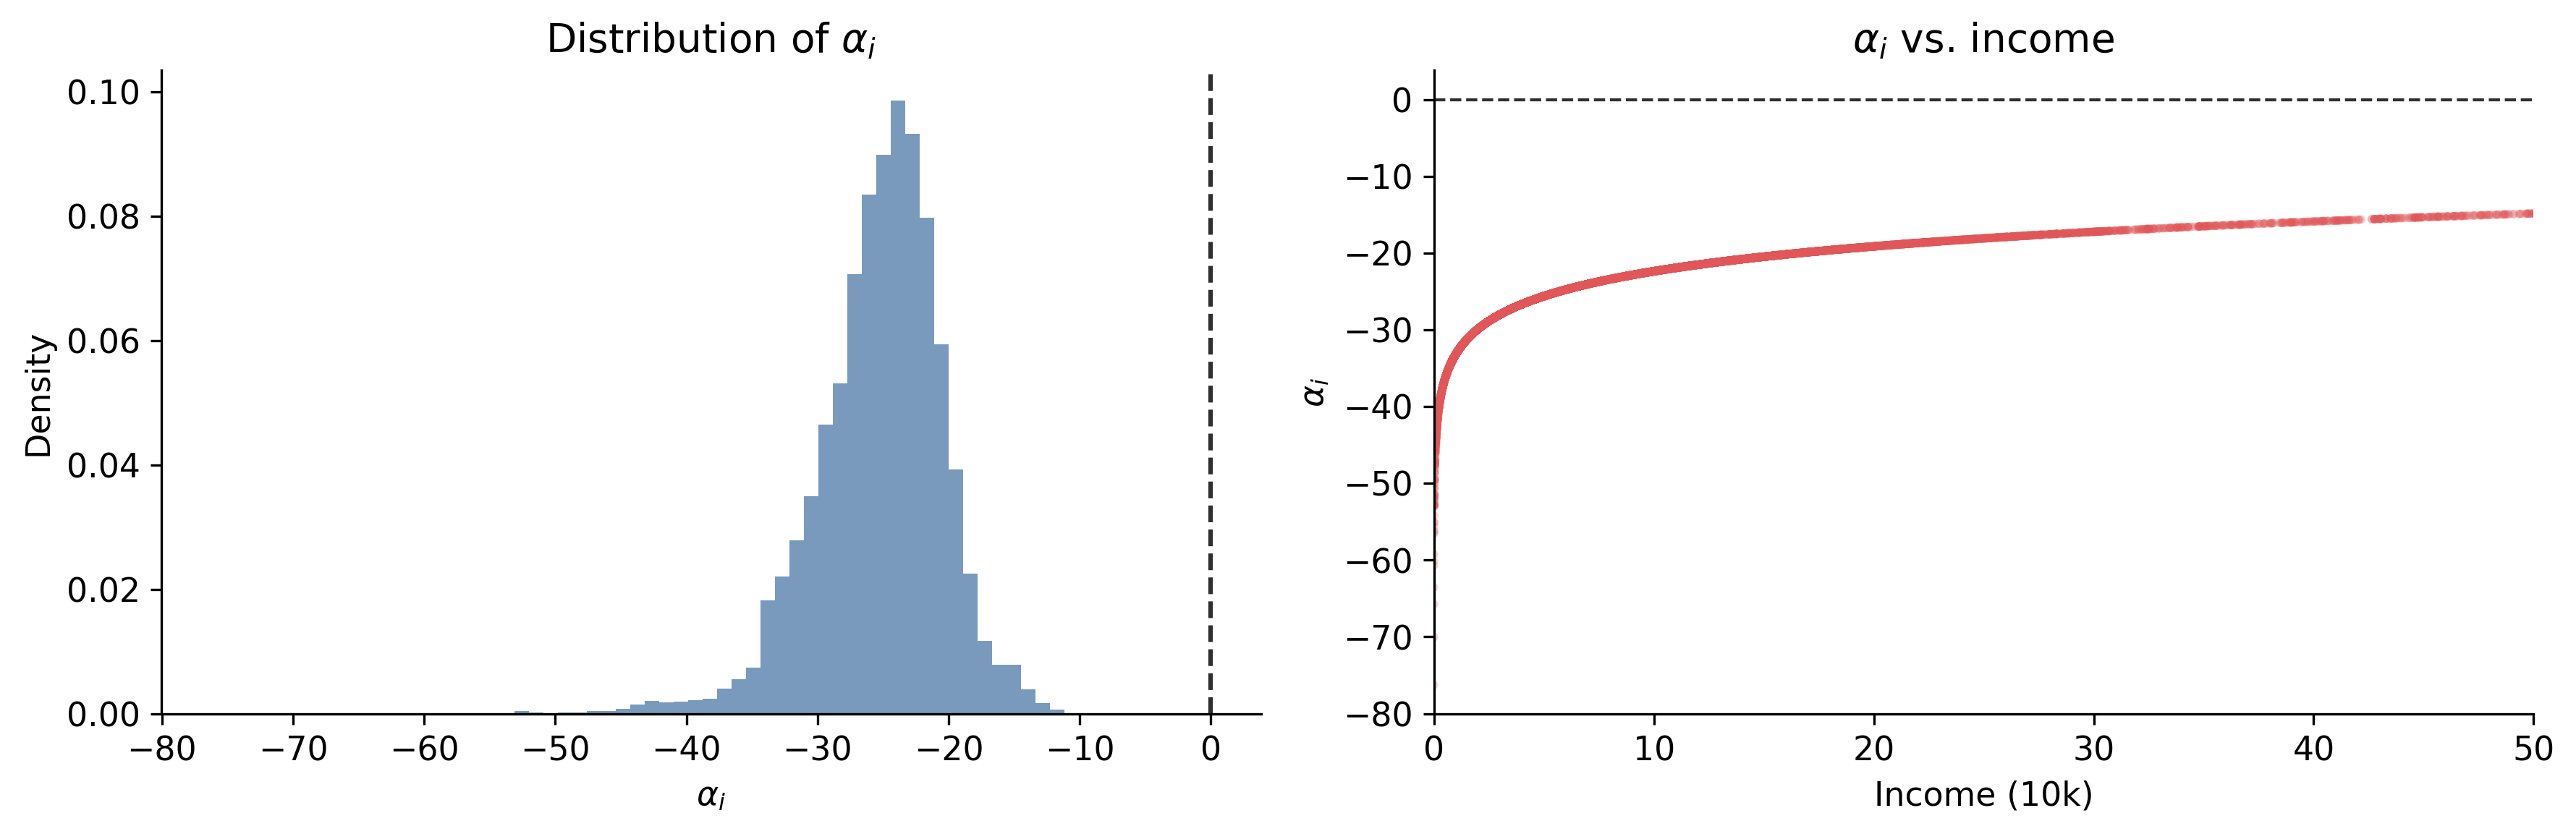
\includegraphics[width=1\linewidth]{generated/graphs/price_coef.png}
    \caption{Distribution of consumer distaste for prices}
    \label{fig:price_coef}
\end{figure}

Our simulated micro moments closely match their empirical counterparts. The moments with the weakest fit are those capturing differences in purchase probabilities and expected purchase prices across income quintiles. This is not surprising, given that the model includes only a single coefficient on log income to govern heterogeneity in preferences for the inside good and price sensitivity. The observed and simulated micro moments are reported in Table \ref{tab:micro_moments}.

\input{generated/tables/micro_moments}

\subsubsection{Elasticities and Markups}
Across the full sample, our demand system implies a share-weighted mean own-price elasticity of \(-6.75\), meaning that a 1\% increase in prices leads to a 6.75\% reduction in sales. In the 2024 market, a common 1\% increase in the price of all vehicles implies a market elasticity of \(-0.420\). Our estimate of the own-price elasticity is in line with the literature, lying between the estimate of \(-5.06\) reported by \cite{grieco_evolution_2024} and the range reported for individual products by \cite{cosar_what_2018}, which spans from \(-14.09\) to \(-15.73\). Our estimate of the market elasticity—the percentage change in total vehicle sales following a 1\% increase in the price of all vehicles—is smaller in magnitude than those typically found in the literature, which are generally closer to \(-1\) (\cite{grieco_evolution_2024}, \cite{allcott_effects_2024}, \cite{berry_automobile_1995}).

These elasticities imply markups and marginal costs, which we recover by inverting equation \eqref{eq:blp_mc} to obtain marginal costs and then computing markups as \((p_j - mc_j)/p_j\). The share-weighted average markup across the full sample is 17.2\%. Figure \ref{fig:markups_dist} presents the distribution of own-price elasticities and markups in the 2024 market.
\begin{figure}
    \centering
    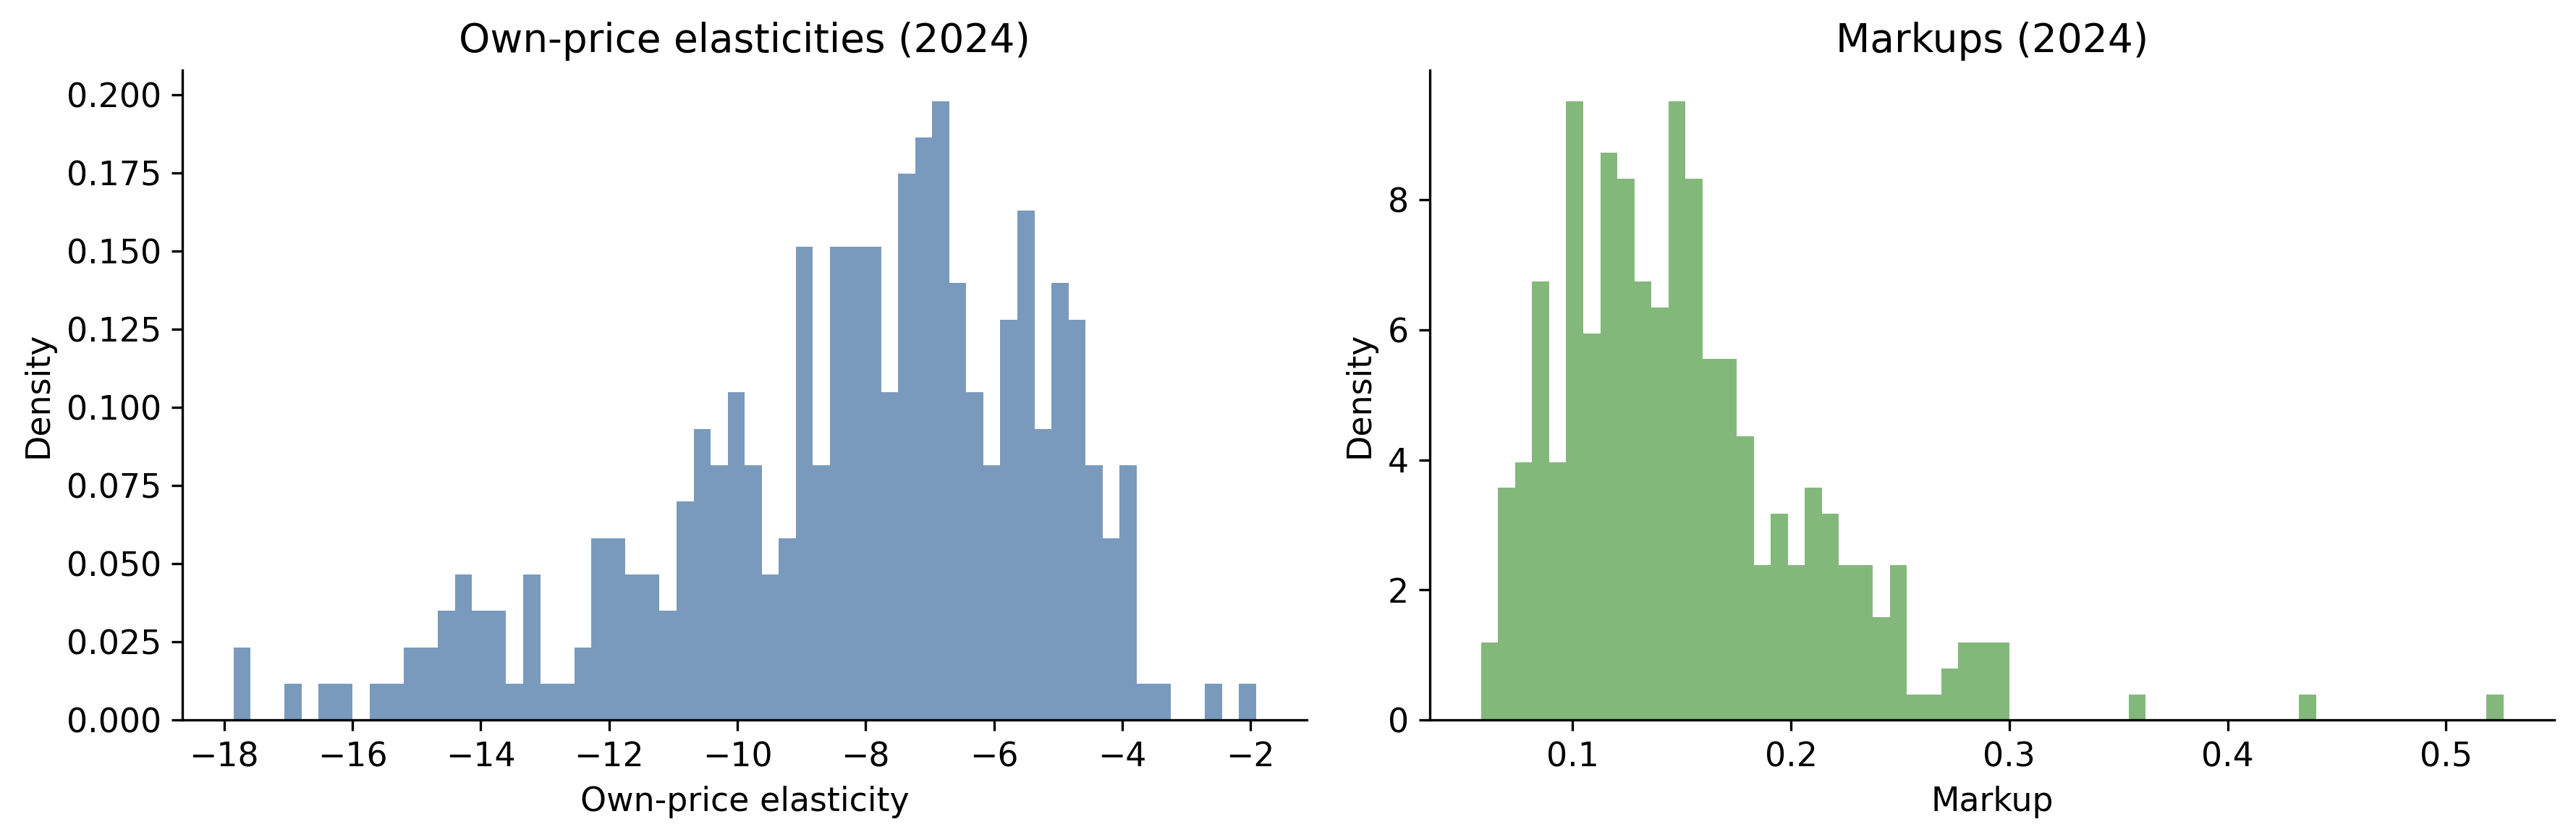
\includegraphics[width=1\linewidth]{generated/graphs/markups_dist.png}
    \caption{Distribution of own-price elasticities and markups, 2024}
    \label{fig:markups_dist}
\end{figure}

\subsubsection{Diversion Ratios}
A key strength of random-coefficients discrete choice models is their ability to generate realistic substitution patterns across products. We rely on these implied substitution patterns to compute changes in consumer and firm welfare in the counterfactual analysis. Here, we assess the plausibility of the model by examining the diversion ratios implied for a set of representative products.

The diversion ratio \(d_{jk}\) is defined as the fraction of consumers who, when switching away from product \(j\) in response to a price change, substitute toward product \(k\) \citep{conlon_empirical_2021}. Formally,
\begin{align}
    d_{jk}
    =
    -\frac{\partial s_{kt} / \partial p_{jt}}{\partial s_{jt} / \partial p_{jt}}.
\end{align}

Table \ref{tab:diversions_top5} reports the diversion ratios for six representative products in the 2024 market. The top alternatives are qualitatively similar to the base product in each panel. In most cases, substitution occurs within the same vehicle category (e.g., electric vehicles, trucks), and the leading substitutes correspond to vehicles that would intuitively be considered close competitors.

\input{generated/tables/diversions_top5}


\subsection{Supply-Side Results}

We present the results for the baseline specification described above, along with an alternative first-differences specification to assess robustness, in Table \ref{tab:cost_side_results}.


% Requires: \usepackage{booktabs,threeparttable}
\begin{table}[!htbp]
\centering
\begin{threeparttable}
\caption{Cost-Side Regressions: Exchange-Rate Shocks and Imported Parts Exposure}
\label{tab:cost_side_results}
\setlength{\tabcolsep}{5pt}
\renewcommand{\arraystretch}{1.12}
\newcommand{\sym}[1]{\ifmmode^{#1}\else\(^{#1}\)\fi}
\begin{tabular}{lcccc}
\toprule
 & \multicolumn{2}{c}{\textbf{Levels}} & \multicolumn{2}{c}{\textbf{First-differences}} \\
\cmidrule(lr){2-3}\cmidrule(lr){4-5}
 & \textbf{(1)} & \textbf{(2)} & \textbf{(3)} & \textbf{(4)} \\
\midrule
$\ln(\text{size})$
  & $0.545$\sym{***} &  & $0.509$\sym{*} &  \\
  & $(0.201)$ &  & $(0.257)$ &  \\
$\ln(\text{weight})$
  & $0.302$\sym{*} &  & $0.402$\sym{*} &  \\
  & $(0.175)$ &  & $(0.222)$ &  \\
$\ln(\text{hp})$
  & $0.189$\sym{**} &  & $0.214$\sym{**} &  \\
  & $(0.082)$ &  & $(0.100)$ &  \\
$\ln(\text{mpg})$
  & $-0.095$ &  & $-0.045$ &  \\
  & $(0.076)$ &  & $(0.069)$ &  \\
$\rho^{(1)}_{f,j,t-1}\cdot \log\!\big(RER^{(1)}_{jt}\big)$
  & $0.598$\sym{**} & $0.674$\sym{***} & $0.445$\sym{**} & $0.607$\sym{**} \\
  & $(0.229)$ & $(0.219)$ & $(0.214)$ & $(0.233)$ \\
\midrule
Make-model FE & Yes & Yes & No  & No  \\
Year FE       & Yes & Yes & Yes & Yes \\
\midrule
Observations  & 374 & 374 & 255 & 255 \\
$R^2$         & 0.979 & 0.975 & 0.144 & 0.050 \\
Within $R^2$  & 0.181 & 0.055 & 0.114 & 0.016 \\
\bottomrule
\end{tabular}
\begin{tablenotes}[flushleft]
\footnotesize
\item \textit{Notes:} The dependent variable is $\ln(\text{costs})$. The real exchange rate is the bilateral real exchange rate between the US and the supplier country, normalized to 1 for each country in 2015; an increase in the $RER$ variable indicates an appreciation of the foreign currency. Standard errors (clustered by make-model) are in parentheses below coefficients.
Significance levels: \sym{*} $p<0.10$, \sym{**} $p<0.05$, \sym{***} $p<0.01$.
\end{tablenotes}
\end{threeparttable}
\end{table}



The preferred specification is reported in column (1), which includes vehicle characteristics as controls. In both the levels and first-differences specifications, we obtain sensible coefficients on the characteristics and a statistically significant coefficient on the interaction between the lagged import share and the real exchange rate. The estimated coefficient of interest implies that, for a domestically assembled vehicle that sources 100\% of its parts from abroad, a 1\% increase in the cost of those parts leads to a 0.601\% increase in the vehicle’s marginal cost.

This estimate is below external assessments of the gross share of vehicle costs attributable to parts. In a case study of General Motors, \cite{helper_management_2014} reports that approximately 70\% of a vehicle’s cost is attributable to parts. In contrast, \cite{menk_methodology_2012} estimates that roughly 71\% of the value of finished vehicles reflects parts costs. In this context, we interpret our estimate as capturing incomplete transmission of foreign input price shocks into recovered marginal costs, reflecting upstream absorption, domestic cost components, and medium-run sourcing adjustments.
%\footnote{ Here, the short run is defined as within the calendar year of the shock.}

\section{Counterfactuals}\label{sec:sec_counterfactuals}
\begin{comment}
    This is a very good instinct, and you’re right: Section 6 is doing too much at once, which makes it feel “kitchen sink” even though every piece is individually defensible. This is a classic issue for strong applied IO papers going to ReStud.

Below I’ll do three things:

Diagnose precisely why Section 6 feels like a kitchen sink

Propose a cleaner conceptual flow for the counterfactuals

Give you a concrete reorganization plan (with section titles and what moves where)

I’ll be blunt where needed, but this is all very fixable.

1. Why Section 6 currently feels like a kitchen sink

The problem is not that you have too many results. It’s that multiple conceptual questions are being answered in parallel rather than sequentially.

Right now, Section 6 is implicitly answering all of the following at once:

What happens with vehicle tariffs?

What happens with parts tariffs?

What happens with both?

What happens with EV subsidies?

What happens to revenue?

What happens across income groups?

What happens across regions?

What happens to EV sales?

Each of these is reasonable — but they are different questions, and the reader isn’t always sure which margin you are isolating at a given moment.

For ReStud, this triggers the reaction:

“I believe the numbers, but I’m not sure what the experiment is.”

2. The principle you should use to reorganize Section 6

Here is the key rule I recommend:

Each subsection should answer exactly one economic question.
Not one policy question — one mechanism question.

Everything else (distribution, EVs, revenue) should be conditional on that mechanism, not interwoven with it.

3. A cleaner, ReStud-style flow for Section 6

Here is a proposed restructuring that keeps all your content but imposes a much clearer logic.

Section 6: Counterfactual Analysis
6.1 Benchmark: Vehicle tariffs only (final-good protection)

Economic question:

What is the incidence of protection when tariffs apply only to final goods?

What goes here:

Vehicle-only tariff results

Price changes

Producer surplus changes

Aggregate consumer surplus

Minimal mention of EVs (only if illustrative)

What stays out:

Parts tariffs

Subsidy repeal

Detailed distributional breakdowns

This section should feel like:

“This is what standard intuition would predict.”

6.2 Intermediate-input tariffs and the reversal of incidence

Economic question:

How does taxing intermediate inputs alter the incidence of protection?

What goes here:

Vehicles + parts tariff

Comparison to 6.1

Emphasis on marginal-cost channel

Firm-level reversals (GM, Ford)

Clear statement: this is where intuition breaks

This is the core contribution section. It should be the longest and cleanest.

6.3 The role of incomplete pass-through

Economic question:

To what extent do sourcing adjustment and upstream absorption mitigate these effects?

What goes here:

Counterfactual with full pass-through vs estimated pass-through

Quantitative attenuation

Clear statement that mitigation ≠ elimination

This section makes your Section 3.3 modeling choice pay off.

6.4 Policy interactions: EV subsidies as an amplifying margin

Economic question:

How do trade policies interact with existing demand-side subsidies?

What goes here:

Stacked tariff + subsidy repeal

EV sales effects

Why EVs are special (input exposure + elastic demand)

Important:
Frame this explicitly as an interaction, not “another scenario.”

6.5 Distributional and regional incidence (conditional results)

Economic question:

Who bears the burden given the mechanisms above?

What goes here:

Income quintiles

Regional maps

Welfare decomposition

This section should begin with language like:

“Conditional on the incidence mechanisms documented above…”

That signals this is not a new mechanism.

6.6 Fiscal implications (short, contained)

Economic question:

How do tariff revenues compare to welfare losses?

This can be very short and possibly merged into 6.2 or 6.5 if space is tight.

4. What you should move out of the main text (if needed)

If the editor pushes for shortening, here is a clean priority list:

Move to appendix first:

Detailed regional maps

Full income-quintile tables

Secondary EV robustness

Keep in main text no matter what:

Vehicle-only vs vehicle+parts comparison

Pass-through attenuation result

One EV interaction result

5. One concrete change that will help immediately

At the start of each subsection in Section 6, add one sentence answering:

What economic question is this subsection answering?

Example:

“This subsection isolates the effect of taxing intermediate inputs by comparing a vehicle-only tariff to a tariff applied to both vehicles and parts.”

This sounds trivial, but it dramatically improves referee comprehension.

Bottom line

You do not need fewer results.
You need a clearer hierarchy of questions.

Right now Section 6 says:

“Here is everything we learned.”

It should instead say:

“Here is the mechanism → here is how it changes → here is who it affects.”

\end{comment}

This section quantifies the equilibrium implications of trade policy by combining the three central components of our framework: consumer substitution across differentiated products, firm pricing under oligopolistic competition, and the transmission of foreign input cost shocks into marginal costs through global value chains. The counterfactuals are designed to isolate how these margins interact to shape prices, quantities, and welfare under alternative tariff and subsidy regimes.

The Trump Administration has prioritized tariffs as a trade policy instrument, implementing new measures affecting imports of automotive parts and finished vehicles. In March 2025, the U.S.\ government announced additional tariffs of 25\% on imported vehicles and automotive components under Section 232 of the Trade Expansion Act of 1962, with preferential rates subsequently applied to imports from the United Kingdom (10\%), Japan (15\%), and South Korea (15\%) (\cite{united_states_congress_section_2025}).

At the same time, the Trump Administration repealed EV subsidies enacted under the Biden Administration’s Inflation Reduction Act (IRA), effective September 2025.

We use our model to evaluate the counterfactual effects of these policy changes by applying them to the simulated 2024 U.S.\ automotive market. A central objective is to disentangle the impacts of the policy package on heterogeneous U.S.\ firms and consumers.

In addition to a baseline scenario featuring no tariffs and the repeal of IRA EV subsidies, we consider five main counterfactual scenarios. These consist of ``subsidy reinstated'' and ``subsidy repealed'' versions of three tariff regimes: (i) no tariffs, (ii) tariffs applied to all imported vehicles and automotive parts, and (iii) tariffs applied to vehicles only, with automotive parts exempted.

The counterfactual results should be interpreted as medium-run outcomes. In our setup, firms can adjust marginal costs through re-sourcing decisions within the same calendar year as the tariff implementation, as described in our cost-side analysis, and can re-optimize product prices. However,  the model does not capture potentially important long-run adjustments in supplier networks or long-run firm responses such as entry and exit decisions in vehicle assembly, parts manufacturing, or product offerings.

Finally, recall that data from the National Highway Traffic Safety Administration do not distinguish between parts sourced from the United States and Canada. As a result, our simulations effectively treat Canadian parts as tariff-exempt in all scenarios. Vehicles assembled in Canada, however, are subject to tariffs on the model.

\subsection{Solution method}

\subsubsection{Counterfactual costs, prices, and shares}

Leveraging the estimation of equation \eqref{eq:costEst}, we model the pass-through of a percentage tariff on intermediate goods to the marginal cost of domestically assembled vehicles as:
\begin{align}
    mc_{j,CF}^{(d)} = mc^{(d)}_{j,2024} (1+  \eta \cdot \rho_{f, j, 2024} \cdot  tariff_{parts})
\end{align}
\noindent where $\rho_{j,2024}$ is the percentage of value of parts imported, $\eta = 0.5980$ is as estimated in \eqref{eq:costEst}. Since we do not fully observe the source locations of foreign parts, we do not allow for country-specific tariff rates for intermediate parts; the full 25\% tariff is applied to all imported parts.

For foreign assembled vehicles, we treat the tariff as increasing the marginal cost of vehicle $j$ and calculate the counterfactual marginal costs as:
\begin{align}
    mc^{(f)}_{j,CF} = mc^{(f)}_{j,2024} (1+  \tau \cdot  tariff_{j,vehicles})
\end{align}

\noindent where in this case the subscript $j$ on tariffs represents the country-specific tariff rate. Here $\tau$ is a parameter that governs the pass-through of full vehicle tariffs to marginal costs. We borrow the estimate from \cite{cosar_what_2018} and set $\tau = 0.682$. As explained by the authors of this paper, $\tau$ being less than one indicates that, even for imported vehicles, a material portion of marginal costs is in addition to the value on which the tariff is imposed, such as marketing, intra-US distribution, and customer relations.

Given the perturbed marginal cost vector $mc_{j,CF} = (mc_{j,CF}^{(d)}, mc_{j,CF}^{(f)})$ in the counterfactual, we re-solve for the equilibrium prices and shares using the contraction mapping algorithm from \cite{morrow_fixed-point_2011}.

\subsubsection{Firm and Consumer Surplus Computation}

\paragraph{Firm surplus:}
We compute firm-level profits using simulated equilibrium prices and shares under each counterfactual scenario. For each product \(j\) in market \(t\), let \(p_{jt}\) denote the equilibrium price, \(c_{jt}\) marginal cost, and \(s_{jt}\) the simulated market share. Product-level per-capita profit is:
\begin{equation}
\pi_{jt} = (p_{jt} - c_{jt}) \cdot s_{jt}.
\end{equation}
Firm-level profits aggregate per-capita profit across products owned by firm \(f\), which are then scaled by market size $M_t$:
\begin{equation}
\Pi_{ft} = M_t\cdot\sum_{j \in \mathcal{J}_f} \pi_{jt}.
\end{equation}
Firm-level changes are computed as differences between counterfactual and baseline values. US producer surplus is the sum of profit changes for US-headquartered firms.

\paragraph{Consumer surplus:}
Consumer surplus is computed using the random-coefficients logit inclusive value, evaluated at simulated equilibrium prices in each market. For consumer \(i\) in market \(t\), we simulate utility for product \(j\):
\begin{equation}
u_{ijt} = \delta_{jt} + \mu_{ijt} + \varepsilon_{ijt},
\end{equation}
as in equation \ref{eq:u_with_delta}. The inclusive value for agent \(i\) is:
\begin{equation}
IV_{it} = \log \left(\sum_{j \in \mathcal{J}_t} \exp(\delta_{jt} + \mu_{ijt}) \right),
\end{equation}
The compensating-variation measure of consumer surplus for agent \(i\) is:
\begin{equation}
CS_{it} = \frac{1}{|\alpha_i|} \, IV_{it},
\end{equation}
with \(\alpha_i\) the consumer-specific marginal utility of price implied by the estimated random coefficients. In practice, we compute \(IV_{it}\) using the simulated draws for \(\mu_{ijt}\) and the equilibrium prices for each scenario, then aggregate over simulated agents using their weights \(w_{it}\) and scale by market size $M_t$:
\begin{equation}
CS_t = M_t \cdot\sum_{i} w_{it} \, CS_{it}.
\end{equation}
We report changes in consumer surplus as:
\begin{equation}
\Delta CS_t = CS^{cf}_t - CS^{0}_t.
\end{equation}

\subsection{Counterfactual Results}

%We now discuss the results of our model in two stages. To isolate the impact of the proposed tariffs, we first consider how the trade counterfactuals affect US firms and consumers with EV subsidies remaining in-place; second, we consider how additionally removing the IRA EV subsidies affects results---it is here that we present results for the full Trump policy package. A summary of our results in Table \ref{tab:cf_summary}.

%e discuss two sets of counterfactuals—changes in tariffs and changes in the IRA EV subsidy—relative to a common baseline in which the IRA EV subsidy is repealed, and no additional tariffs are imposed. We begin by holding EV subsidies off and comparing two tariff regimes: (i) a 25\% tariff on imported finished vehicles only, and (ii) a 25\% tariff on both imported vehicles and imported parts. We then examine the welfare implications of re-enacting the IRA EV subsidy. Table \ref{tab:cf_summary} summarizes the headline outcomes across these counterfactuals. For each scenario, we report the consumer surplus (overall and by income quantile), producer surplus, tariff revenue, fiscal cost of the EV subsidy, and changes in prices, markups, and production.

%We understand the mechanism of tariff policies, we look into the change in marginal costs, prices, markups, and market share for the US-assembled and foreign-assembled vehicles.  To understand how tariff policies impacts different firms/distributional aspect we producer-surplus changes across firms. In particular, we focus on the counterfactual with no EV subsidy and a 25\% tariff on foreign vehicles, which isolates the effects of the 25\% tariff policy. For this case, we examine firm-level adjustments in prices, marginal costs, markups, and market shares, and we document the implied changes in profits across all firms. We also run the counterfactuals of different types of tariffs with the EV subsidy. Results of all the five counterfactuals along with the baseline are compiled in the Appendix table \ref{tab:cf_summary_full}.

We discuss two sets of counterfactuals—changes in tariffs and changes in the IRA EV subsidy—relative to a common baseline in which the IRA EV subsidy is repealed, and no additional tariffs are imposed. We begin by holding EV subsidies off and comparing two tariff regimes: (i) a 25\% tariff on imported finished vehicles only, with some country-specific lower rates, and (ii) a 25\% tariff on both imported vehicles and imported parts.\footnote{We only apply country-specific tariff rates to final vehicles; all parts receive the 25\% tariff.} We then examine the welfare implications of reinstating the IRA EV subsidy. Table \ref{tab:cf_summary} summarizes the headline outcomes across these counterfactuals. For each scenario, we report consumer surplus (overall and by income quintile), US producer surplus, tariff revenue, the fiscal cost of the EV subsidy (when applicable), and changes in prices, markups, and production.

We next unpack the mechanisms behind these aggregate results. We first decompose the tariff effects by assembly location, examining how marginal costs, prices, markups, and market shares adjust for US-assembled versus foreign-assembled vehicles. We then study the distribution of producer-side impacts across firms by reporting firm-level profit changes. To isolate the incidence of the tariff policy itself, we emphasize the counterfactual with the EV subsidy repealed and a 25\% tariff on imported vehicles. Finally, we repeat the tariff analysis under the reinstated EV subsidy. Results for all five counterfactuals, together with the baseline, are reported in Appendix Table \ref{tab:cf_summary_full}.

\begin{table}[!htbp]
\centering
\caption{Counterfactual Tariff and Subsidy Scenarios: 2024 Market Outcomes}
\label{tab:cf_summary}
\small
\setlength{\tabcolsep}{6pt}
\renewcommand{\arraystretch}{1.10}
\begin{threeparttable}
\begin{tabular}{lccc}
\toprule
 & \multicolumn{2}{c}{Without Subsidy} & With Subsidy \\
\cmidrule(lr){2-3}\cmidrule(lr){4-4}
 & C1: Vehicles-only & C2: Parts \& vehicle & C3: No tariff \\
\midrule
$\Delta$ Price (avg, \%) & 5.23 & 8.89 & -0.06 \\
$\Delta$ Markup (avg \%) & -0.5 & -0.7 & -0.0 \\
$\Delta$ US Producer Surplus (b USD) & 1.04 & -2.06 & 1.80 \\
CS $\Delta$ total (b USD) & -14.116 (-4.3\%) & -29.793 (-9.1\%) & 10.055 (3.1\%) \\
CS $\Delta$ Q1 (b USD) & -0.512 (-6.8\%) & -1.089 (-14.5\%) & 0.053 (0.7\%) \\
CS $\Delta$ Q2 (b USD) & -1.540 (-5.6\%) & -3.161 (-11.5\%) & 0.746 (2.7\%) \\
CS $\Delta$ Q3 (b USD) & -2.659 (-6.1\%) & -5.673 (-13.0\%) & 1.797 (4.1\%) \\
CS $\Delta$ Q4 (b USD) & -3.629 (-5.0\%) & -7.686 (-10.6\%) & 2.981 (4.1\%) \\
CS $\Delta$ Q5 (b USD) & -5.775 (-3.3\%) & -12.184 (-6.9\%) & 4.477 (2.5\%) \\
$\Delta$ vehicles sold (m) & -0.381 & -0.792 & 0.201 \\
EV share (\% sales) & 3.22 & 3.20 & 7.39 \\
US-assembled share (\% sales) & 65.9 & 57.7 & 53.5 \\
$\Delta$ US assembled (m) & 1.170 & 0.049 & 0.144 \\
Tariff revenue (b USD) & 14.55 & 40.29 & 0.000 \\
EV subsidy cost (b USD) & 0.000 & 0.000 & 6.68 \\
$\Delta$ Net US outcomes (b USD) & 1.48 & 8.44 & 5.17 \\
\bottomrule
\end{tabular}
\end{threeparttable}
\end{table}


\subsubsection{Trade policies}

\paragraph{Consumer and firm welfare}
As shown in Table \ref{tab:cf_summary}, expanding the policy from a 25\% tariff on imported finished vehicles only (C1) to a 25\% tariff that also applies to imported parts (C2) substantially amplifies the equilibrium cost shock. Average prices increase by 5.2\% under the vehicles-only tariff (C1), but by 8.9\% when parts are included (C2). Consistent with the larger price increase, total vehicle sales fall by 0.38 million in C1 versus 0.79 million in C2.

These larger price and quantity effects translate into much larger consumer welfare losses. Aggregate consumer surplus falls by \$14.1 billion in C1, compared to \$29.8 billion in C2. The losses are borne disproportionately by higher-income households in absolute dollar terms in both counterfactuals: the top income quintile (Q5) accounts for around 40\% of the consumer welfare loss. This pattern is consistent with higher-income consumers accounting for a larger share of vehicle purchases (and therefore a larger share of total dollar surplus), even if lower-income households are more price-sensitive and may experience larger losses relative to their baseline surplus.

On the production side, the difference between C1 and C2 is also sharp. Under the vehicles-only tariff (C1), US producer surplus rises by \$1.0 billion and US-assembled output increases by 1.17 million vehicles, consistent with substitution away from imported finished vehicles toward domestically assembled alternatives. Once imported parts are also tariffed (C2), this substitution channel is muted: US-assembled output rises by only 0.05 million vehicles, and US producer surplus falls by \$2.06 billion, indicating that higher input costs for domestic assembly offset the demand-diversion gains from taxing imported final vehicles.

Finally, tariff revenues are large in the broader-tariff scenario: \$14.55 billion in C1 versus \$40.29 billion in C2. Mechanically, this raises the measured “net US outcomes” (CS + US PS + tariff revenue) from +\$1.48 billion in C1 to +\$8.44 billion in C2. Importantly, however, these net gains come from revenue collection and do not, by themselves, eliminate the large consumer surplus losses—whether households are ultimately better off depends on how tariff revenues are recycled (or not) back to consumers and/or domestic firms.

\paragraph{Change by assembly location}

Figure \ref{fig:origin_metrics_tariffs_no_subsidy} decomposes the equilibrium effects of the two tariff counterfactuals (both evaluated with the IRA EV subsidy repealed) by vehicle assembly location (US-assembled vs.\ foreign-assembled). Each bar reports the change in prices, marginal costs, markups (percentage points), and market shares (percentage points) relative to the no-tariffs, EV subsidy repealed baseline. Panels (a) and (b) show the results for counterfactual C1 (25\% tariff on foreign-assembled vehicles only) and C2 (25\% tariff on vehicles and parts), respectively. The vehicle-only tariff primarily affects foreign-assembled models: their marginal costs rise by 13.68\% and their prices by 10.87\%. The fact that the price response is smaller than the cost shock implies incomplete pass-through, and correspondingly, foreign-assembled markups compress by 1.94 pp. A notable feature is that US-assembled prices change little (+0.27\%), whereas foreign-assembled prices increase sharply. Under Nash–Bertrand pricing, this implies that domestic assemblers gain little additional pricing power: competition among US models and substitution to the outside option constrain markups. This is consistent with the outside good holding a large baseline share (49.3\%) and meaningful diversion out of the market. The tariff induces a sharp reallocation of demand across assembly locations: foreign-assembled market share falls by 7.04 pp, while US-assembled market share rises by 5.31 percentage points (with the remaining 1.73 percentage points shifting to the outside option, since shares are defined over the full market, including non-purchase).


Panel (b) of figure \ref{fig:origin_metrics_tariffs_no_subsidy} shows the counterfactual results when the tariff is extended to imported parts, resulting in the propagation to domestically assembled vehicles as well. US-assembled marginal costs increase by +8.09\%, and prices rise by +7.01\%, again implying incomplete pass-through and a 0.82 percentage point decline in US-assembled markups. Foreign-assembled vehicles continue to experience larger increases (+13.68\% in costs and +11.02\% in prices) and a larger markup decline (1.83 pp), indicating that the overall burden remains heavier on foreign-assembled models. Unlike C1, however, the gain in US-assembled market share is much smaller (+0.22 pp), while foreign-assembled market share falls by 3.82 pp, implying a substantial shift toward the outside option. Intuitively, once imported parts are taxed, domestic assembly becomes more expensive, limiting the extent to which US-assembled vehicles can absorb demand diverted away from imports; as a result, the policy operates more like a broad cost shock that contracts the market rather than a pure reallocation from foreign to domestic assembly.

Overall, these assembly-location-level mechanisms align with the aggregate patterns: C1 mostly reallocates demand from foreign-assembled vehicles toward US assembly, while C2 raises costs for both, compresses markups across the board, and shifts a larger share of consumers toward non-purchase.


\begin{figure}[!htbp]
\centering
\begin{subfigure}[t]{0.48\linewidth}
    \centering
    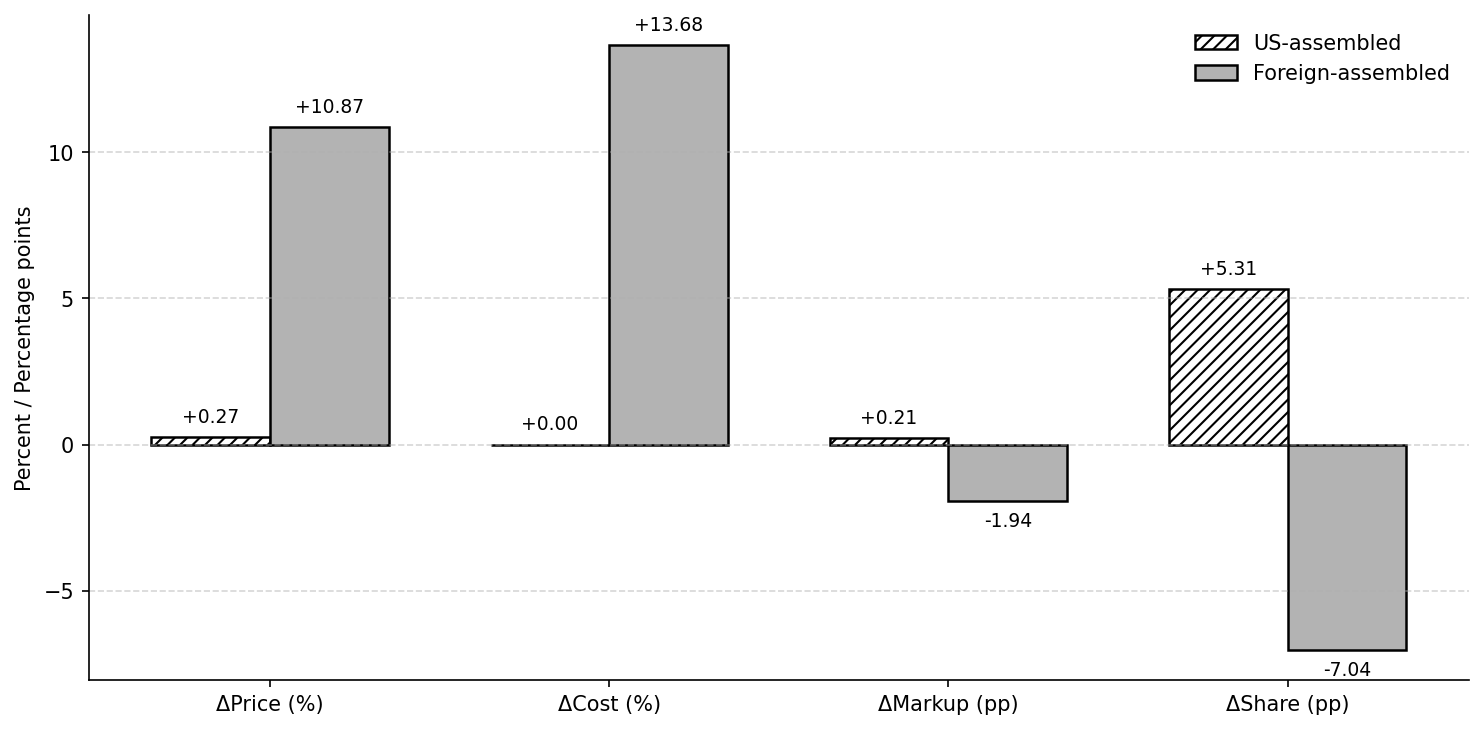
\includegraphics[width=\linewidth]{generated/graphs/origin_metrics_vehicles_only_tariff__no_subsidy.png}
    \caption{\textbf{Counterfactual: Vehicle-only tariff}}
    \label{fig:origin_metrics_vehicles_only_tariff__no_subsidy}
\end{subfigure}\hfill%
\begin{subfigure}[t]{0.48\linewidth}
    \centering
    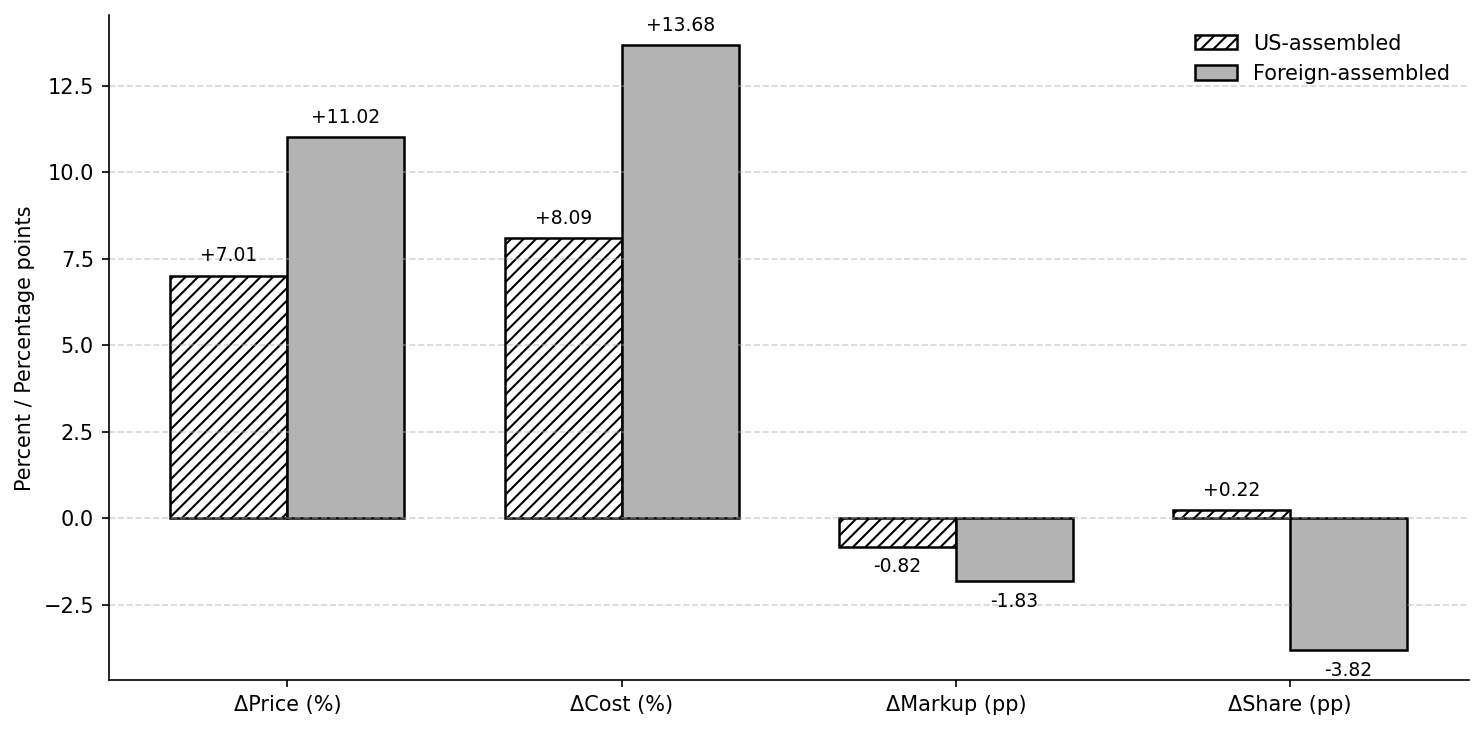
\includegraphics[width=\linewidth]{generated/graphs/origin_metrics_parts_and_vehicles_tariff__no_subsidy.png}
    \caption{\textbf{Counterfactual: Parts and vehicle tariffs}}
    \label{fig:origin_metrics_parts_and_vehicles_tariff__no_subsidy}
\end{subfigure}
\caption{Changes by assembly-location: Tariff counterfactuals}
\label{fig:origin_metrics_tariffs_no_subsidy}

\captionsetup{font=footnotesize, justification=raggedright, singlelinecheck=false}
\caption*{\textit{Notes:} These figures compare changes in prices, costs, markups, and market shares by assembly location of the vehicle (US-assembled vs.\ foreign-assembled). Panel (a) reports counterfactual C1 (25\% tariff on imported vehicles only) and Panel (b) reports counterfactual C2 (25\% tariff on imported vehicles and imported parts). Each change is relative to the ``no-tariffs, EV subsidy repealed'' baseline. ``Assembled'' categorization is distinct from firm headquarters location. These assembly-location-level mechanisms align with aggregate patterns: C1 mostly reallocates demand from foreign-assembled vehicles toward US assembly, while C2 raises costs for both, compresses markups across the board, and shifts a larger share of consumers toward non-purchase.}
\end{figure}


\paragraph{Profit by firms}

%\hl{Figure 8: profits by firms: Tariff counterfactuals: Alternate way to show in a single graph but a messy one: because we want to show how does the firm wise profits are impacted by C1 and C2, we can have all this in a single plot. A scatter plot with change in profits from C1 on X and C2 on Y. We might miss out on firms names, but we can add that in the text. }

Table \ref{tab:cf_summary} reports that the change in aggregate US producer surplus increases under the vehicle-only tariff (C1) but turns negative when the tariff is extended to parts (C2). Figure \ref{fig:ps_scatter_pct_more} shows that these aggregate patterns conceal substantial firm-level heterogeneity. It plots percentage changes in firm-level profits relative to the baseline under two counterfactual tariff scenarios: C1 (a 25\% tariff on imported finished vehicles only) on the x-axis and C2 (a 25\% tariff applied to both imported vehicles and imported parts) on the y-axis.

Three patterns stand out. First, larger firms (larger bubbles) tend to lie closer to the origin, indicating smaller percentage changes in profits. Second, under C1, most non-U.S. firms (blue) experience profit declines—25 firms overall have negative changes—reflecting the direct impact of tariffs on imported vehicles. A few exceptions, such as Honda, Acura, Nissan, and BMW, benefit due to their substantial US assembly presence. Third, extending tariffs to parts (C2) reverses gains for many firms, particularly U.S.-headquartered manufacturers (e.g., Chevrolet, GMC, and Ford) that are more exposed to imported inputs. In contrast, firms with lower reliance on foreign parts (e.g., Tesla, Jeep, Honda, and Toyota) are more likely to benefit.

Finally, the quadrant structure highlights heterogeneity in tariff incidence. Many foreign firms lie in the bottom-left quadrant (losers under both policies), while several US firms lie in the bottom-right quadrant (gaining under C1 but losing under C2), underscoring the importance of input sourcing in shaping the incidence of protection. Appendix figure \ref{fig:ps_scatter_pct_less} shows the labels of the remaining firms (with a lesser market share). Appendix figure \ref{fig:ps_scatter_usd_more} plots the change in profit in USD instead of the percentage value.

\begin{figure}[!htbp]
\centering
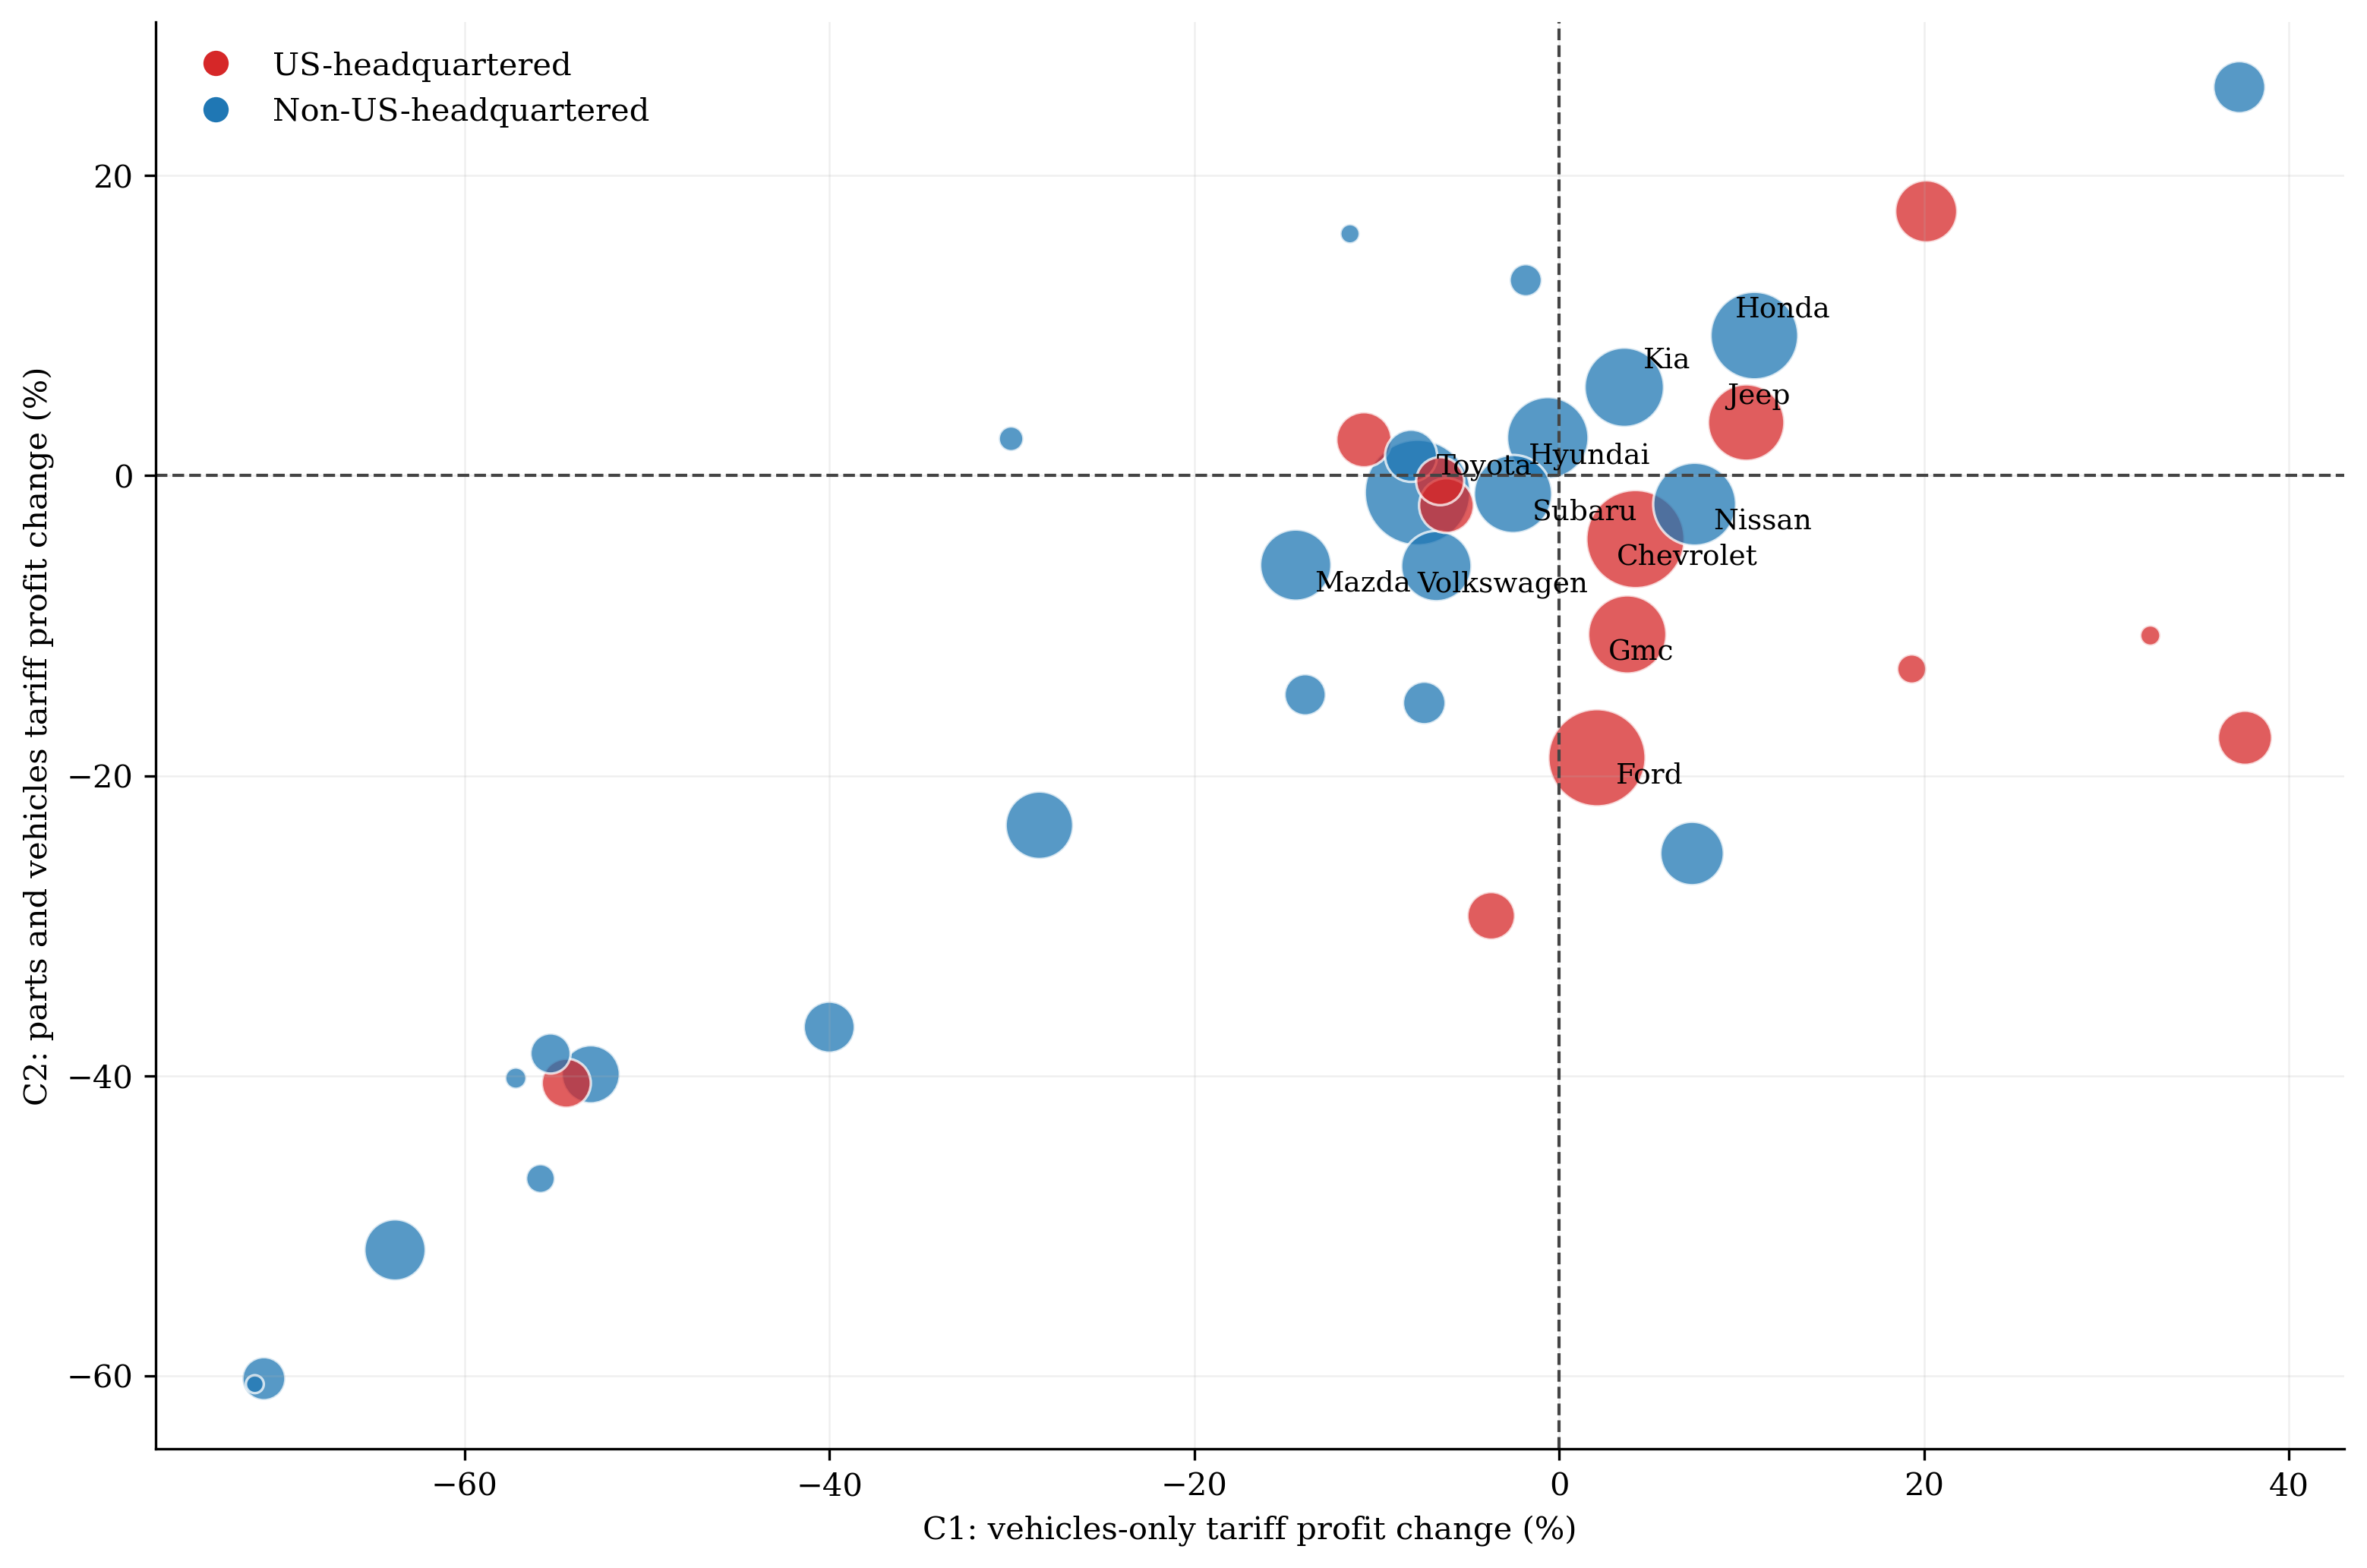
\includegraphics[width=1\textwidth]{generated/graphs/z_scatter_pct_more.png}
\caption{\textbf{Percentage profit changes across firms under tariff counterfactuals}}
\label{fig:ps_scatter_pct_more}
%\captionsetup{font=footnotesize, justification=raggedright, singlelinecheck=false}
\caption*{\textit{Notes:} The figure plots percentage changes in firm-level profits relative to the baseline under two counterfactual tariff scenarios: C1 (25\% tariff on imported finished vehicles only) on the x-axis and C2 (25\% tariff applied to both imported vehicles and imported parts) on the y-axis. Each bubble represents one of the 38 firms in the sample, of which 13 are U.S.-headquartered. Bubble size is proportional to the firm's market share. Colors indicate firm headquarters (red: U.S.; blue: non-U.S.), while assembly locations may differ from headquarters, reflecting global production networks.}
\end{figure}




\begin{comment}
Under C1 (panel a), profit gains are concentrated among firms that benefit from demand diversion away from tariffed imported finished vehicles. Honda exhibits the largest gain among non-U.S.-headquartered firms, and Tesla also records a sizable profit increase. Among U.S.-headquartered firms, Jeep and Chevrolet experience moderate gains, while several others see small positive effects. In contrast, a number of firms incur losses under C1. Ford experiences the largest decline in profits, followed by Mercedes, GMC, Lexus, BMW, and Audi. These losses reflect either substantial exposure to imported finished vehicles or product portfolios that compete directly with models benefiting from demand reallocation.

When the tariff is expanded to cover imported parts (C2, panel b), the distribution shifts markedly toward losses. The inclusion of parts raises marginal costs even for domestically assembled vehicles, weakening the diversion channel that generated winners under C1. Firms that gained under C1—such as Honda and Tesla—continue to post positive profit changes under C2, but their gains are attenuated. Meanwhile, losses deepen and broaden across the market. Mercedes experiences the largest decline in C2, followed by Toyota, Lexus, Audi, Hyundai, and Chrysler. Notably, Ford’s losses under C1 are substantially reduced under C2, reflecting the fact that the broader tariff redistributes the burden more evenly across firms rather than concentrating it on specific portfolios.

Overall, the comparison between panels illustrates the mechanism at work: C1 (vehicle-only tariff) primarily reallocates demand across assembly locations, creating distinct winners and losers, whereas C2 (parts and vehicle tariff) operates more like a broad-based cost shock that compresses markups and reduces profitability more widely.

\begin{figure}[!htbp]
    \centering
    % ---------------- Panel A ----------------
    \begin{subfigure}{1\linewidth}
        \centering
        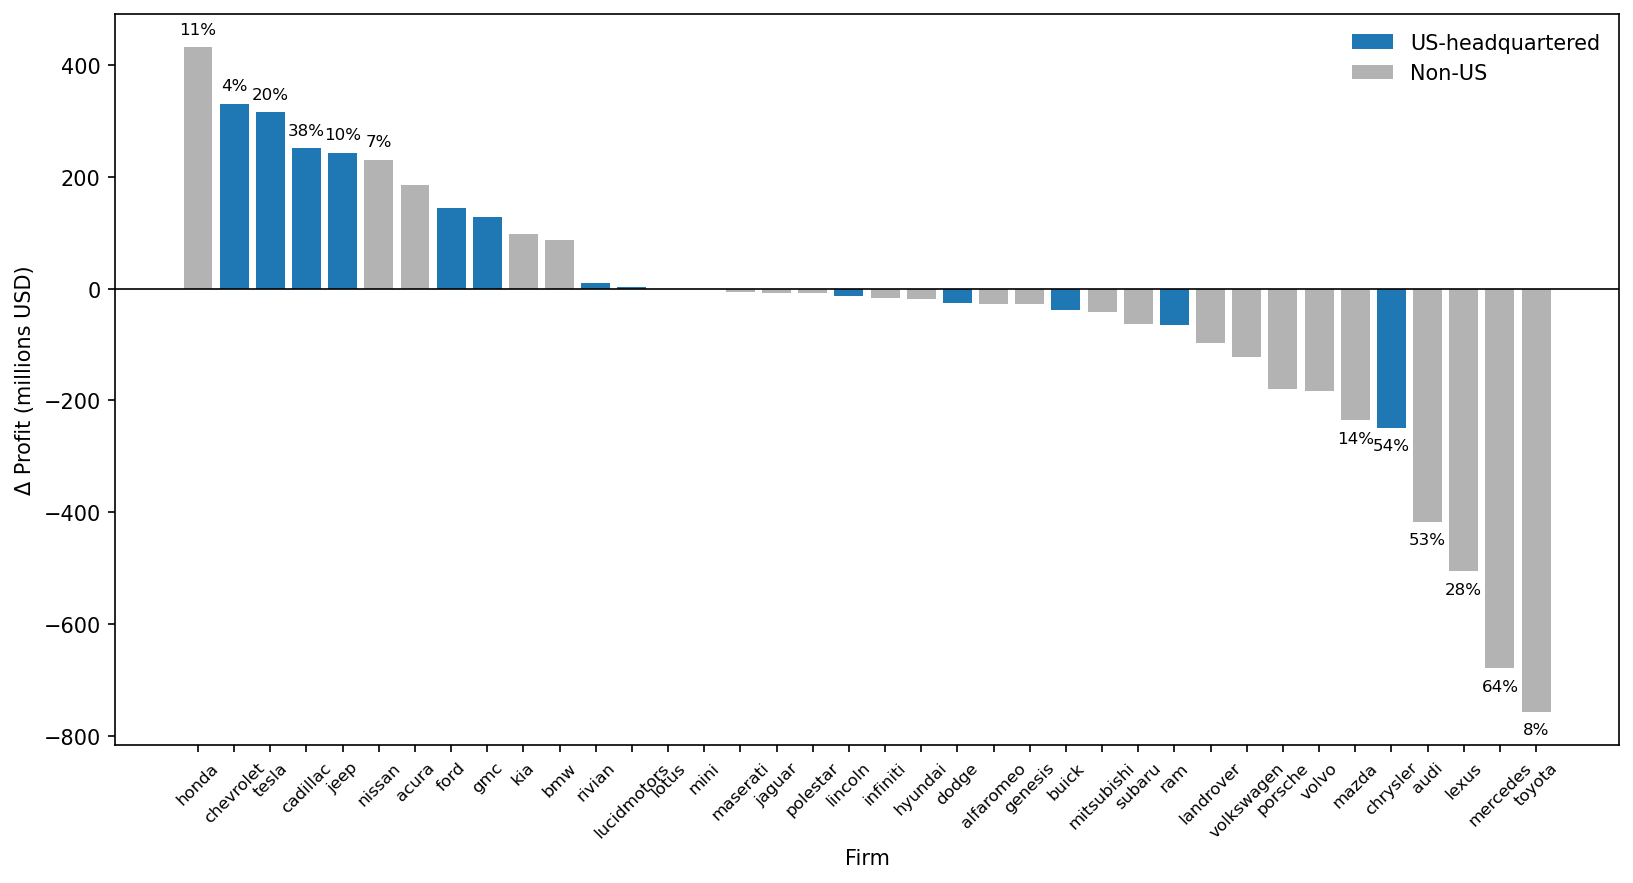
\includegraphics[width=0.9\linewidth]{generated/graphs/profit_changes_vehicles_only_tariff__no_subsidy.png}
        \caption{Firm profit changes: Vehicle-only tariff (C1)}
        \label{fig:profit_changes_vehicles_only_tariff__no_subsidy}
    \end{subfigure}
%    \vspace{0.6em}
    % ---------------- Panel B ----------------
    \begin{subfigure}{1\linewidth}
        \centering
        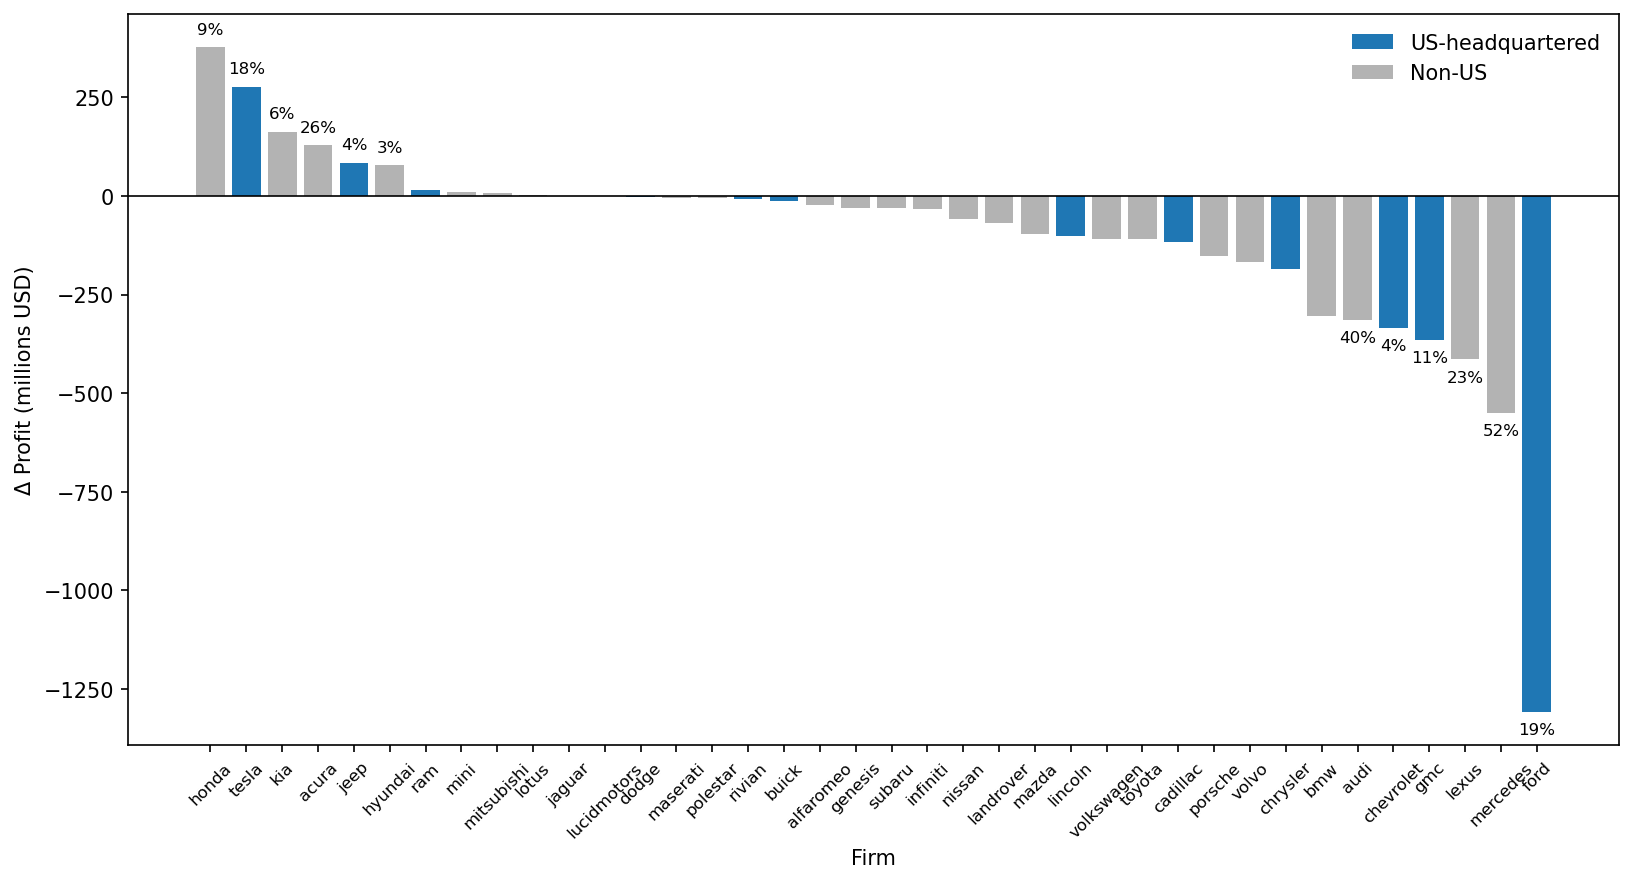
\includegraphics[width=0.9\linewidth]{generated/graphs/profit_changes_parts_and_vehicles_tariff__no_subsidy.png}
        \caption{Firm profit changes: Vehicle and Once imported parts are also tariffed (C2)parts tariffs (C2) }
        \label{fig:profit_changes_parts_and_vehicles_tariff__no_subsidy}
    \end{subfigure}
\caption{Firm profit changes: Tariff counterfactuals}
    \label{fig:profit_changes_tariffs_no_subsidy}
    \captionsetup{font=footnotesize, justification=raggedright, singlelinecheck=false}
    \caption*{\textit{Notes:} Each bar reports the change in firm profits (millions of USD 2015) relative to the
    ``no-tariffs, without EV subsidy'' baseline. Bars are colored by firm headquarters location (US-headquartered vs.\ non-US).
    Bar labels report the corresponding percentage change in firm profits. Firms are ordered from the largest profit increase to the largest profit decrease within each panel. }
\end{figure}
\end{comment}

Additional results are reported in the Appendix Figures. Appendix Figure \ref{fig:profit_change_vs_import_share} highlights heterogeneity in producer-side impacts by relating US-headquartered firms' profit changes (relative to the no-tariffs, EV subsidy repealed baseline) to their exposure to imported inputs, measured by the sales-weighted imported-parts share in their US-assembled vehicles. Appendix Figure \ref{fig:cs_map_parts_and_vehicles_tariff__with_subsidy} maps the state-level distribution of consumer-surplus changes under the parts-and-vehicles tariff with the EV subsidy reinstated, showing that consumer impacts are geographically broad but uneven across states. Finally, Appendix Figure \ref{fig:assembly_map_tariffs_no_subsidy} visualizes how tariff counterfactuals reallocate vehicle production across assembly locations, reporting counterfactual production levels and the corresponding percentage change from baseline.

%Moved to appendix for now  \paragraph{State-based impacts} Here, we extend our analysis of consumer and firm impacts to the state level. State-level consumer welfare varies through two channels: first, the distribution of incomes across states affects state-average consumer welfare impacts through income-based distaste for prices channel; second, regional preferences for electric vehicles, trucks, and SUVs affect the welfare implications of policies at the division level. Figure \ref{fig:cs_map_parts_and_vehicles_tariff__with_subsidy} demonstrates the geographical spread of consumer surplus losses under the full tariff scenario. The geographic spread of the parts-exempt tariff impacts is qualitatively similar (though lower in magnitude).


\subsubsection{EV subsidy reinstatement}
We now examine the welfare implications of reinstating the IRA EV subsidy and report how the resulting welfare changes are distributed across income quantiles. Table \ref{tab:cf_summary} summarizes the headline outcomes across all counterfactuals. %For each scenario, the table reports average price changes; aggregate consumer surplus (overall and by income quintile); US producer surplus; changes in total sales and US-assembled production; the fiscal cost of the EV subsidy; and the implied net US welfare change.
In C3 (no tariffs, EV subsidy in place), the policy operates primarily as a demand-side stimulus with almost no effect on average prices (-0.06\%). Table \ref{tab:cf_summary} shows that the subsidy increases consumer surplus by \$10.1b and US producer surplus by \$1.8b, alongside a modest expansion in market activity (+0.20m vehicles sold) and +0.144m additional US-assembled vehicles. The consumer gains are skewed toward higher-income households in dollar terms—Q5 gains \$4.48b versus \$0.05b for Q1—reflecting that higher-income consumers account for a larger share of vehicle purchases. Accounting for the fiscal cost of the program (\$6.68b), the net US outcome is \$5.17b.

%\hl{maybe a figure like Fig 7, but instead of assembly-location, do it by the engine type (getting subsidy or not.)}

On the producer side, reinstating the EV subsidy generates pronounced heterogeneity in firm outcomes. Figure \ref{fig:profit_changes_no_tariff_no_subsidy} plots the distribution of profit changes across firms and shows that Tesla is the largest beneficiary, with additional gains for US-based EV producers such as Jeep and Cadillac. This dispersion is consistent with the subsidy differentially raising demand for qualifying domestic EV models, shifting purchases away from unsubsidized ICE options, foreign (unsubsidized) EVs, and the outside good.

\begin{figure}
    \centering
    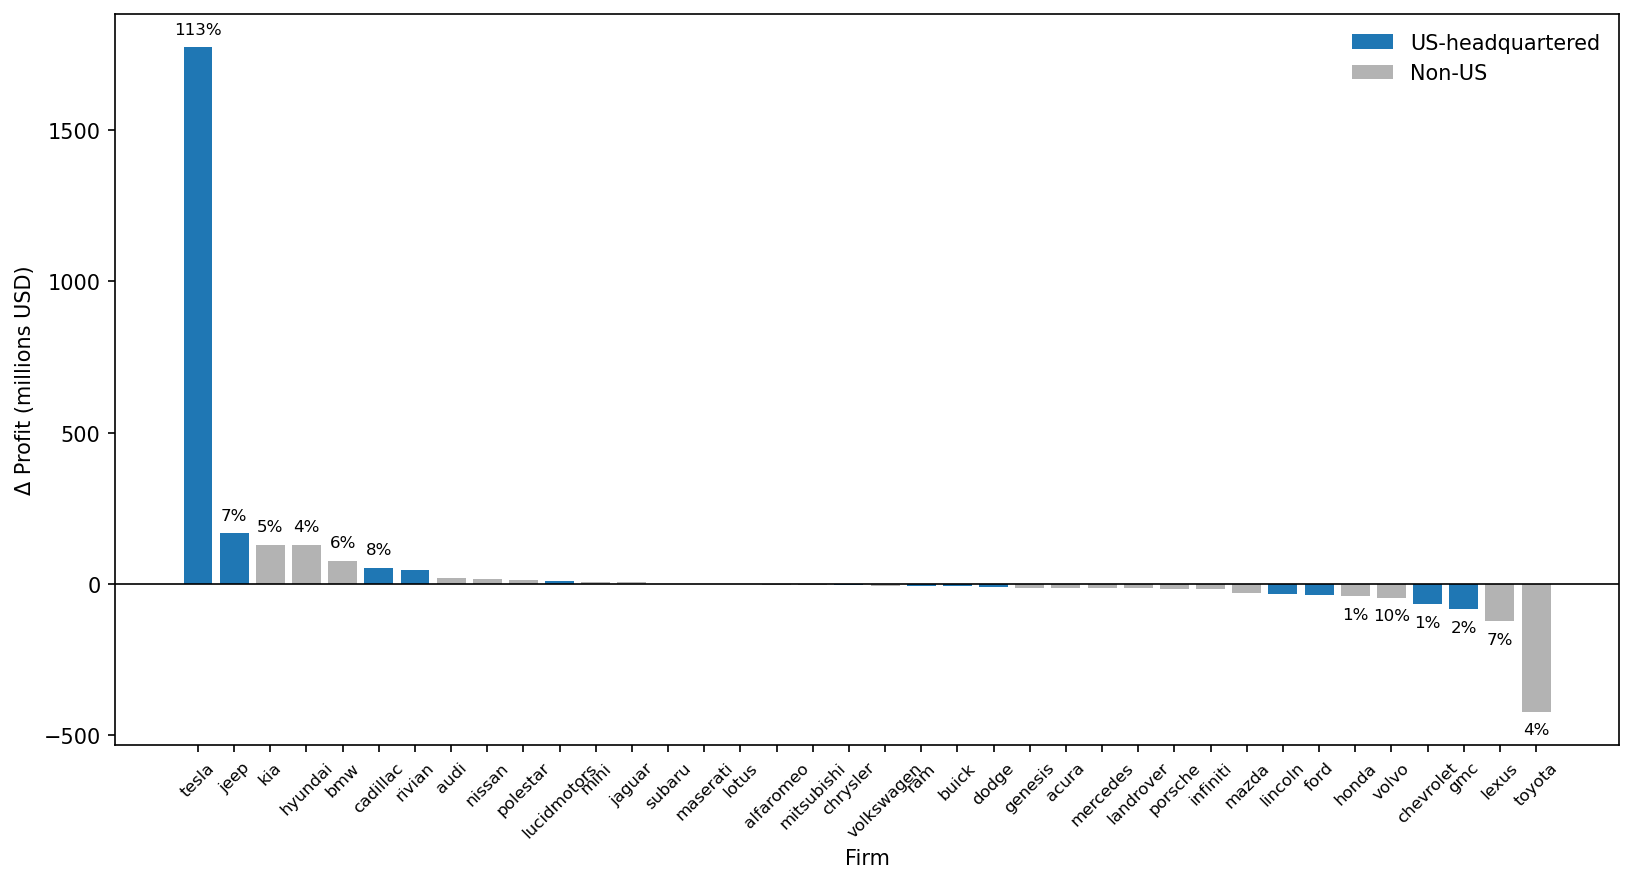
\includegraphics[width=.8\linewidth]{generated/graphs/profit_changes_no_tariff__with_subsidy.png}
    \caption{Firm profit changes: No tariffs, EV subsidy reinstated (C3)}
    \caption*{\textit{Notes:} Bar height is profit change in millions of USD 2015 compared to the 'no-tariffs, EV subsidy repealed' baseline. Bar labels are the corresponding \% change in firm profits.}
    \label{fig:profit_changes_no_tariff_no_subsidy}
\end{figure}

\paragraph{State-based impacts}
%We show only the no-tariff, EV subsidy re-enactment maps to isolate the effect of the subsidy itself; these effects are smaller in magnitude than the tariff counterfactuals.

Reinstating the EV subsidy generates a geographically broad increase in consumer welfare. Figure \ref{fig:cs_map_no_tariff__no_subsidy} shows that the median state experiences a consumer surplus gain of roughly $2.5\%$, with an interquartile range of about $1.9$--$3.1\%$. Gains are larger in a small set of states and are concentrated in regions with a stronger preference for EVs---most notably Oregon ($+8.4\%$), Washington ($+5.6\%$), California ($+5.8\%$), Alaska ($+7.1\%$), and Hawaii ($+7.3\%$). These differences reflect heterogeneity in regional EV preferences, incomes, and the corresponding distaste for price changes.

%Removing the EV subsidy generates a geographically broad, but relatively modest, decline in consumer welfare. Figure \ref{fig:cs_map_no_tariff__no_subsidy} shows that most states experience consumer surplus losses on the order of roughly $0.6$---$1.8\%$ in percentage terms. Losses are somewhat larger in a small set of states and are concentrated in regions with a stronger preference for EVs---most notably the Pacific states of Oregon ($-4.6\%$), Washington ($-3.0\%$), and California ($-3.1\%$), and Alaska ($-3.9\%$). Each of these Pacific states shares the same EV preference in our model; the difference in welfare losses comes from heterogeneity in incomes and corresponding distaste for price increases.

%The manufacturing impact primarily falls on the EV-producing states of California and Texas, with modest gains for many of the other assembler-states, in particular Illinois. Figure \ref{fig:assembly_map_no_tariff__no_subsidy} isolates how subsidy removal changes the distribution of US vehicle assembly across producing states, holding tariffs at zero.


\begin{figure}
    \centering
    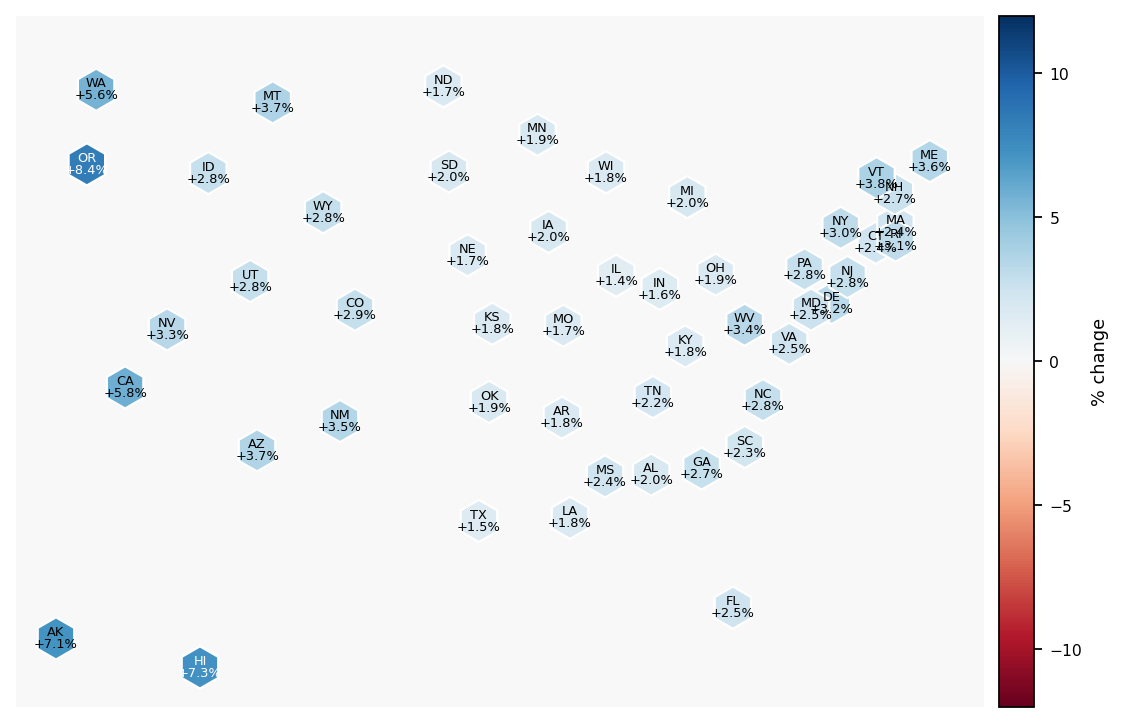
\includegraphics[width=0.75\linewidth]{generated/graphs/cs_map_no_tariff__with_subsidy.png}
    \caption{State consumer surplus impacts: No tariffs, EV subsidy reinstated}
    \captionsetup{font=footnotesize, justification=raggedright, singlelinecheck=false}
    \caption*{\textit{Notes:} Consumer surplus change is relative to the 'no-tariffs, EV subsidy repealed' baseline. Labels for Rhode Island and Delaware have been removed.}
    \label{fig:cs_map_no_tariff__no_subsidy}
\end{figure}


%A fuller account of manufacturing impacts for all scenarios is given in Table \ref{tab:plant_location_changes}.

% REMOVED: state-by-state manufacturing and CS changes. Available in /tables if required.

%%% START: NEW SECTION 6 %%%
\begin{comment}
%# don't need this section.
\subsection{Economic interpretation and incidence mechanisms}
The counterfactual results highlight a set of equilibrium mechanisms that are not specific to the automobile market, but arise more generally in differentiated-products industries with market power and fragmented production. This subsection interprets the results through the lens of these mechanisms and clarifies why taxing intermediate inputs fundamentally alters the incidence of protection.

In a standard setting with differentiated products and oligopolistic pricing, tariffs on imported final goods tend to benefit domestic producers by shifting demand away from foreign competitors. Our results show that this intuition can fail once domestically assembled goods rely on imported intermediate inputs. When parts are taxed, domestic producers experience a marginal-cost increase that scales with their exposure to foreign inputs. Because this cost shock applies to all units sold, it weakens domestic firms’ competitive positions precisely in the segments where they would otherwise gain from demand reallocation. As a result, protection aimed at foreign producers can reduce domestic producer surplus, even when domestic firms retain market power and substitution toward domestic products remains imperfect.

An important feature of the results is that firms are unable to fully offset these cost increases through higher markups. Under Nash-Bertrand pricing with differentiated products, markups depend on substitution patterns and the elasticity of demand faced by each product. In our setting, imported and domestically assembled vehicles are imperfect substitutes, and the outside option captures a substantial share of demand. These features limit firms’ ability to raise prices without losing sales, so parts tariffs compress markups rather than translating one-for-one into higher prices. This markup compression amplifies the adverse profit effects for firms with high imported-input exposure.

Allowing for incomplete pass-through of foreign input cost shocks moderates, but does not eliminate, these effects. Economically, incomplete pass-through reflects a combination of upstream cost absorption and medium-run sourcing adjustments within existing production structures. While these margins dampen the immediate impact of tariffs on marginal costs, they do not sever the link between global input prices and domestic production costs. Consequently, the qualitative incidence patterns—particularly the dependence of firm-level outcomes on imported-input exposure—remain intact even when pass-through is substantially below one.

The interaction between tariffs and EV subsidy removal further illustrates how cost-side and demand-side policies jointly shape incidence. Electric vehicles are disproportionately affected because they combine relatively high exposure to imported inputs with demand that is especially sensitive to price-based incentives. Removing EV subsidies raises the effective price of EVs without materially affecting average vehicle prices, inducing sharp demand shifts away from EV models. When combined with tariffs that raise production costs, this interaction magnifies producer losses for EV-oriented firms and accelerates the contraction of EV sales. More generally, policy interactions are likely to be most consequential in market segments characterized by both high input exposure and elastic demand.

Taken together, these mechanisms imply that the incidence of trade policy cannot be inferred from final assembly location alone. In industries with global value chains, what matters for both firm and consumer outcomes is the degree to which production costs are exposed to foreign inputs and the extent to which firms can adjust prices in response. Policies that appear protective when viewed through the lens of final goods trade can impose substantial costs on domestic producers once intermediate inputs and market structure are taken into account. This logic extends beyond automobiles to other sectors with fragmented production and differentiated products, including electronics, machinery, and clean energy technologies.

\end{comment}

\section{Conclusion}\label{sec:sec_conclusion}

This paper studies the incidence of trade policy in a differentiated-products market with market power and global value chains. Using the U.S.\ automobile industry as a laboratory, we show that exposure to imported intermediate inputs fundamentally alters how tariffs affect prices, profits, and welfare.
Our counterfactual analysis yields three key results. First, tariffs on imported vehicles increase U.S.\ producer surplus by about \$1 billion but reduce consumer surplus by roughly \$14 billion. Second, extending tariffs to imported parts reverses these gains: consumer losses roughly double and U.S.\ producer surplus declines by about \$2.1 billion. %, reflecting higher marginal costs for firms exposed to foreign inputs.
These aggregate effects mask substantial heterogeneity: firms with greater exposure to imported parts experience losses, whereas those relying more on domestic inputs are better able to increase profits. Third, reinstating EV subsidies increases consumer surplus by about \$10.1 billion and raises U.S.\ producer surplus by about \$1.8 billion.

%When domestically assembled goods rely on foreign parts, protection that targets both final goods and intermediate inputs can raise domestic producers’ marginal costs and reverse the competitive gains they would otherwise obtain from tariffs on imported final goods alone.


Our results highlight that the reversal in producer surplus for the domestic firms upon expanding the tariffs on the parts also arises from the interaction of three forces: substitution across differentiated products, oligopolistic pricing, and cost exposure through global value chains.

% dropping it. Explained it enough already.
%Vehicle-only tariffs primarily operate through demand reallocation, shifting sales toward domestically assembled products. Once intermediate inputs are taxed, however, cost shocks scale with firms’ reliance on imported parts and apply to all units sold, weakening domestic firms’ competitive positions. %Because firms face elastic demand and competition from both foreign producers and the outside option, they are unable to fully pass these cost increases through to prices, leading to markup compression and, for many firms, lower profits.

%Allowing for incomplete pass-through of foreign input cost shocks moderates these effects but does not eliminate them. Medium-run sourcing adjustments and upstream cost absorption dampen the transmission of tariffs into marginal costs, yet the qualitative incidence patterns remain tightly linked to firms’ input exposure. As a result, final assembly location alone is an insufficient statistic for evaluating the effects of protection in industries with fragmented production.

%The interaction between tariffs and EV subsidy removal further illustrates how cost-side and demand-side policies jointly shape incidence. Electric vehicles are disproportionately affected because they combine high exposure to imported inputs with demand that is especially sensitive to price-based incentives. Stacking tariffs with subsidy repeal sharply contracts EV sales and redistributes producer surplus toward firms less exposed to both imported inputs and EV demand, underscoring the importance of evaluating trade and industrial policies in combination rather than in isolation.

Although our empirical analysis focuses on automobiles, the mechanisms we document are not specific to that sector. Many industries affected by recent trade policy—including electronics, machinery, and clean energy technologies—feature differentiated products, market power, and heavy reliance on imported intermediate inputs. In such settings, policies that tax inputs as well as final goods are likely to reshape marginal costs and competitive positions in ways that differ from intuition based solely on final-goods trade. More broadly, our findings underscore that evaluating the incidence of trade policy requires explicit attention to global value chains and the interaction between cost exposure and market structure.

%\include{demand}
%\include{cost}
%\include{counterfactuals}
%\include{conclusion}


\input{generated/references.bbl}

\newpage
\appendix\
\counterwithin{figure}{section}         % reset figure counter at each \section
\renewcommand{\thefigure}{\thesection\arabic{figure}}  % prints A1 not A.1

\section{Appendix Figures}\label{sec:appendix_fig}

\begin{figure}[H]
    \centering
    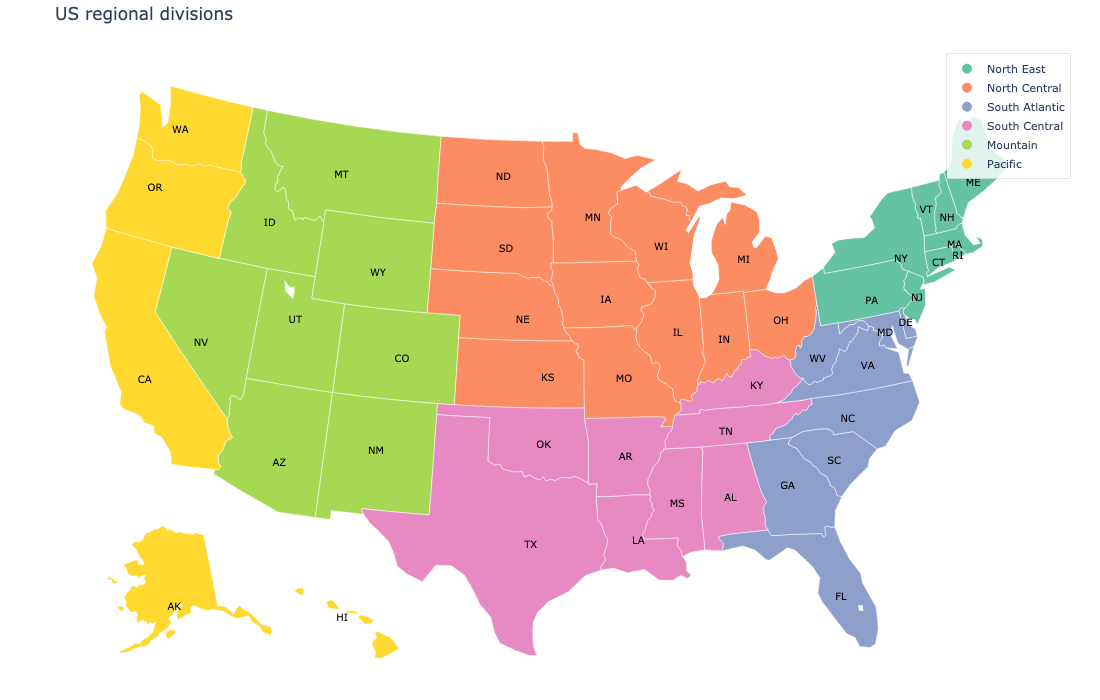
\includegraphics[width=0.8\linewidth]{generated/graphs/div_map.png}
    \caption{US regional divisions}
    \label{fig:div_map}
\end{figure}
\clearpage

\begin{figure}[!htbp]
    \centering
    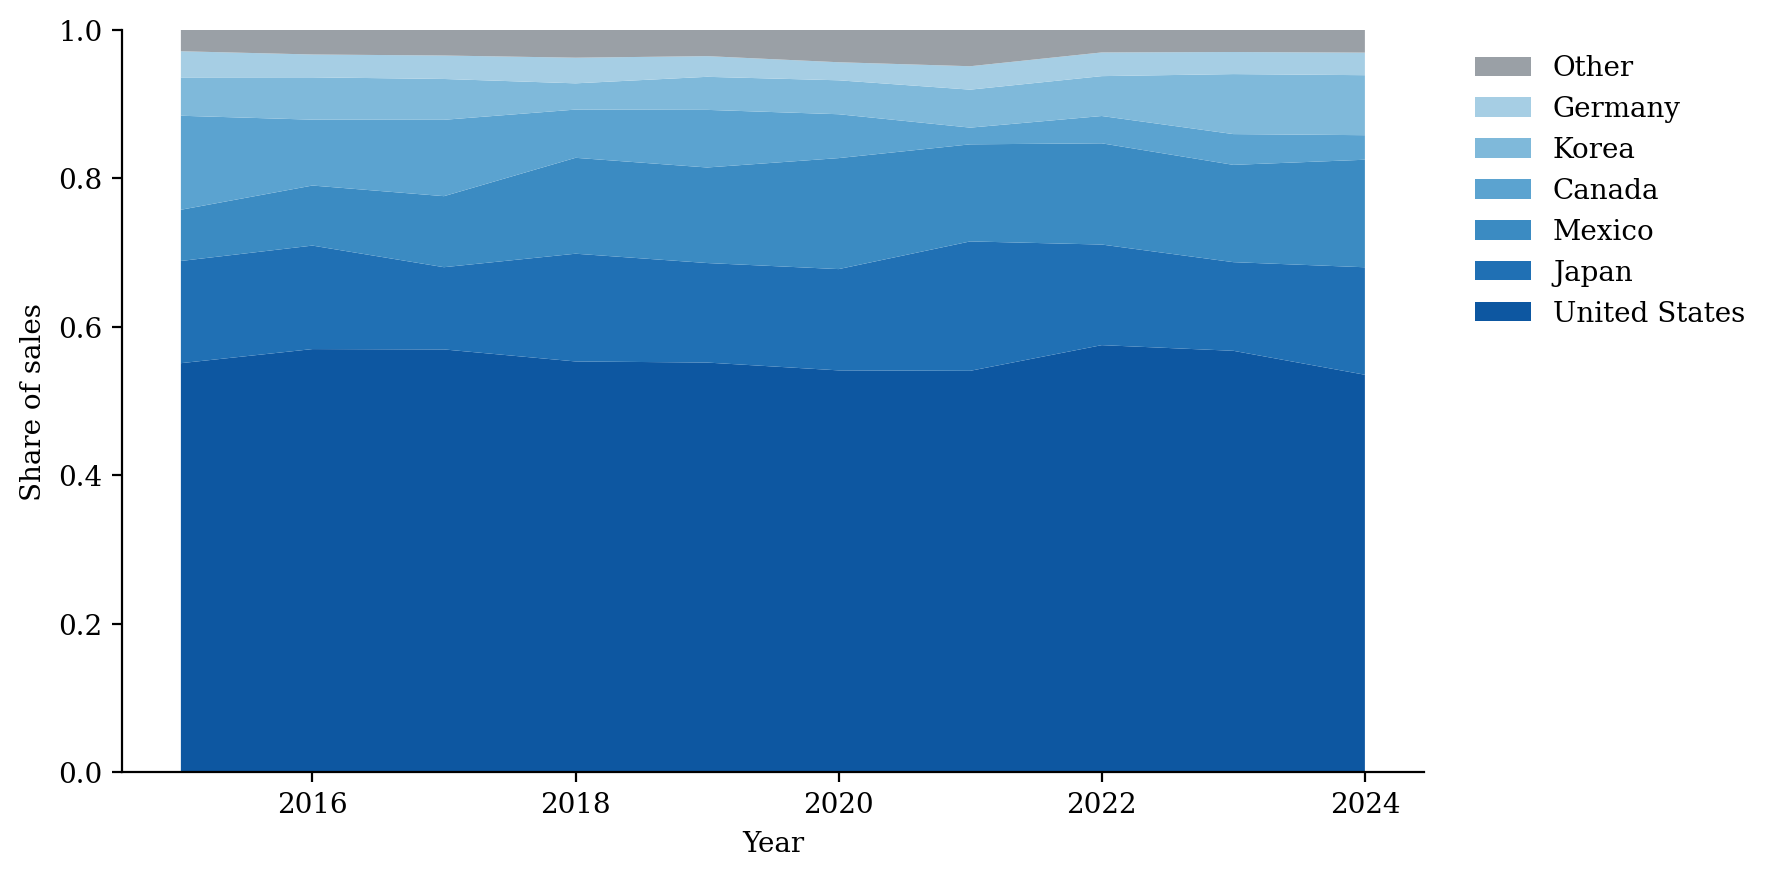
\includegraphics[width=0.8\linewidth]{generated/graphs/sales_weighted_sources_by_year.png}
    \caption{Assembly location (country) of vehicles sold in the United States}
    \label{fig:sales_sources}
    \begin{flushleft}
    \footnotesize
    \textit{Notes:} The figure shows the distribution of assembly locations for vehicles sold in the United States, weighted by sales, over time. It illustrates the importance of foreign production in supplying the U.S. market and the evolution of global production patterns.
    \end{flushleft}
\end{figure}

\begin{figure}
    \centering
    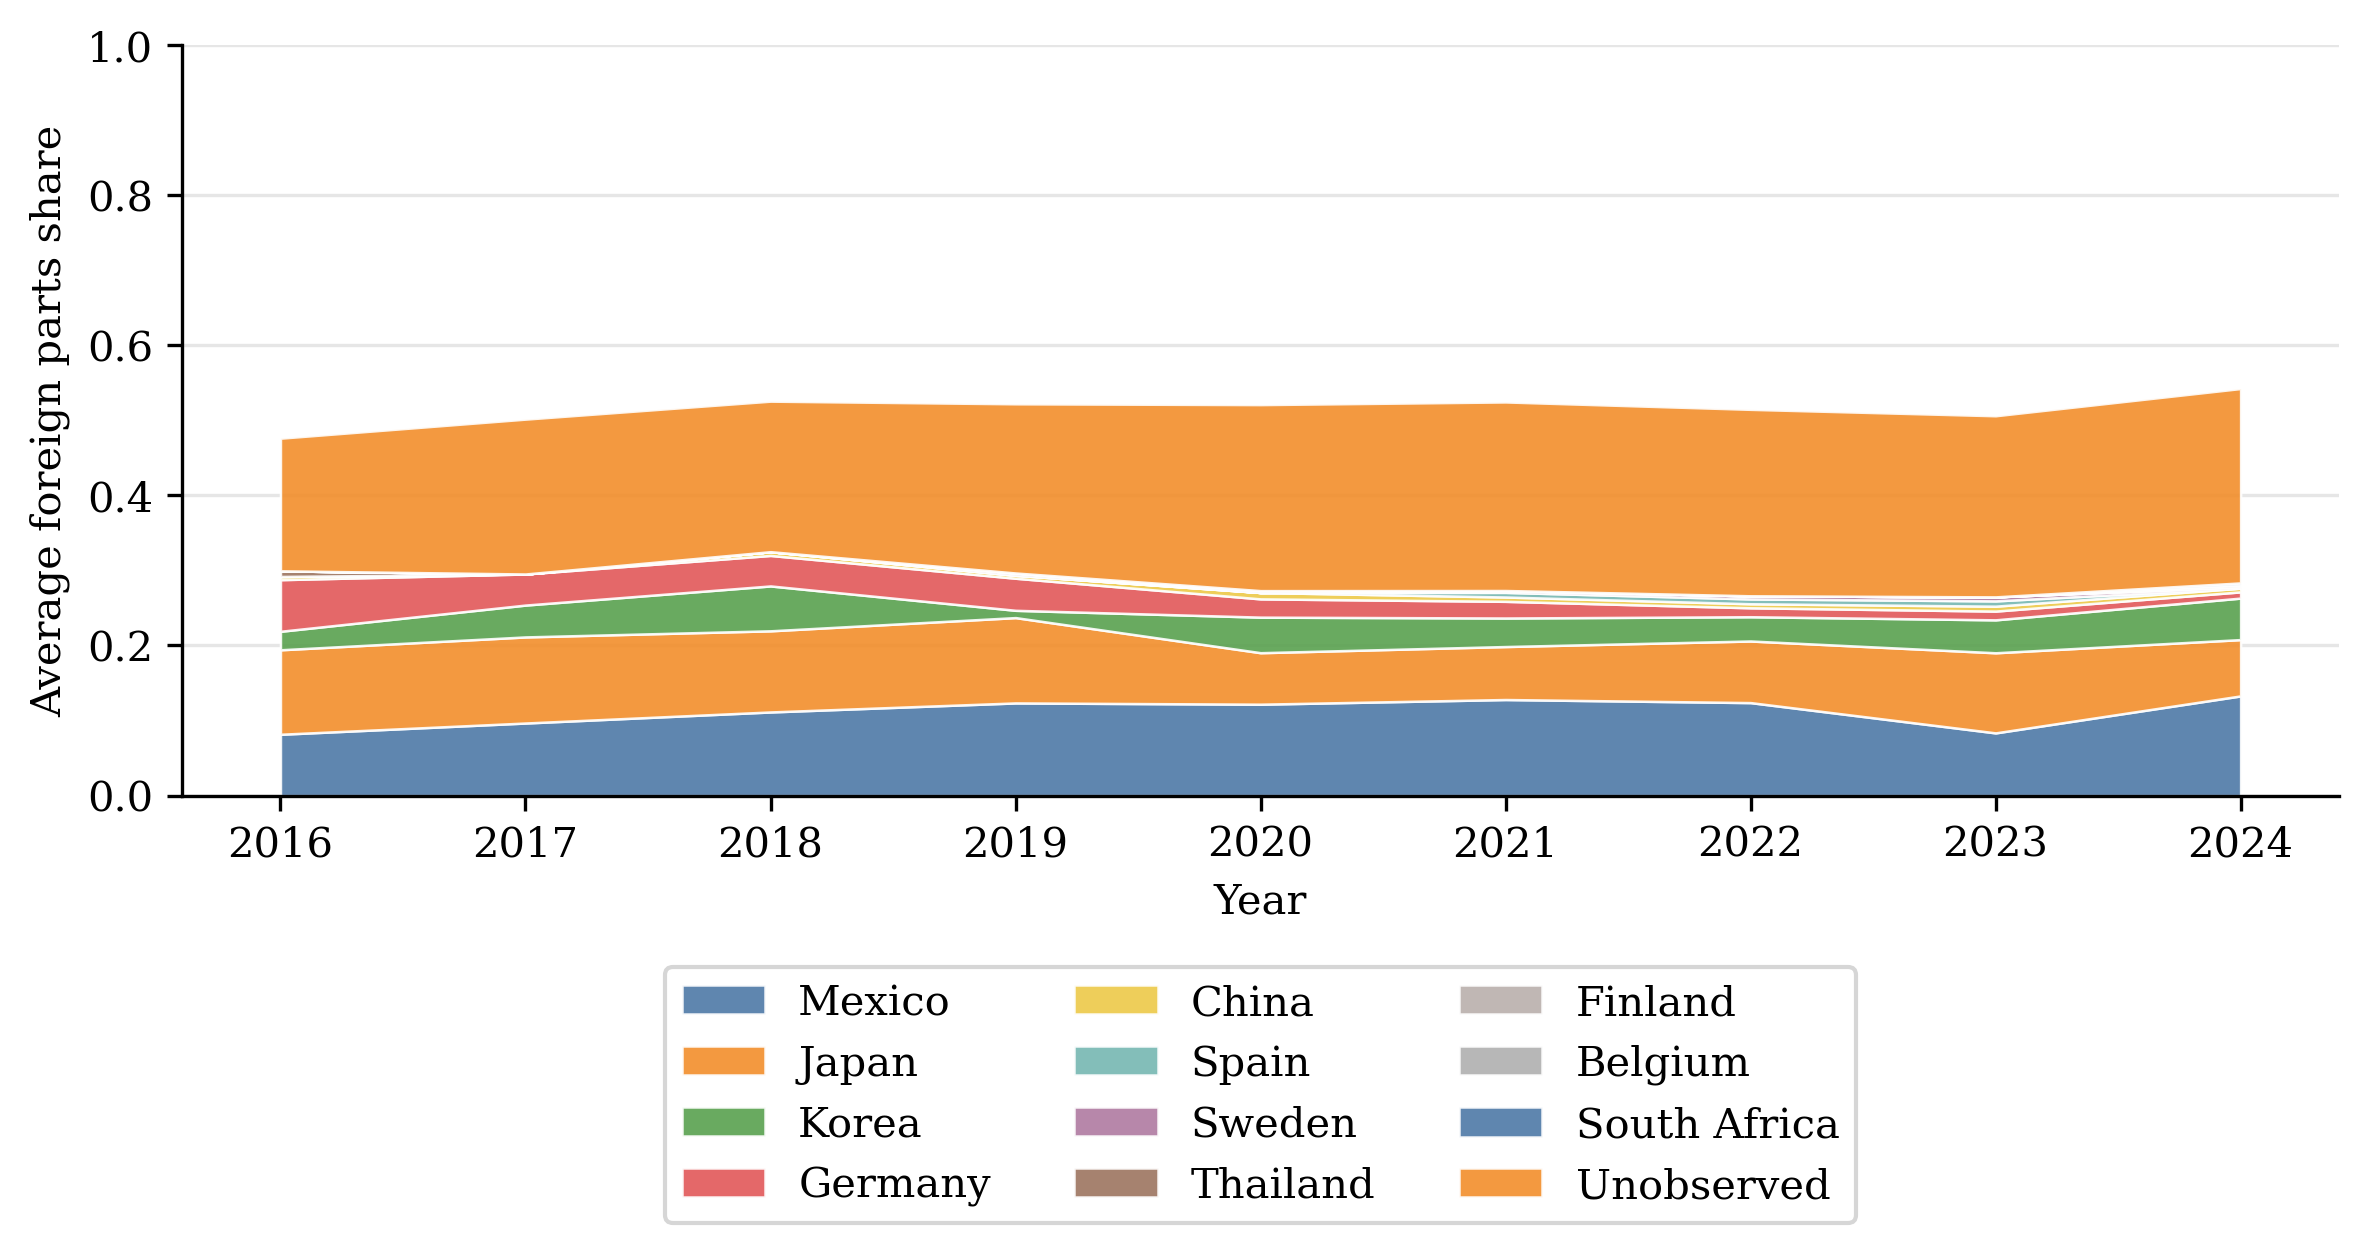
\includegraphics[width=0.8\linewidth]{generated/graphs/foreign_parts.png}
    \caption{Observed foreign sources of vehicle parts}
    \label{fig:sources}
\end{figure}
\clearpage


\begin{figure}
    \centering
    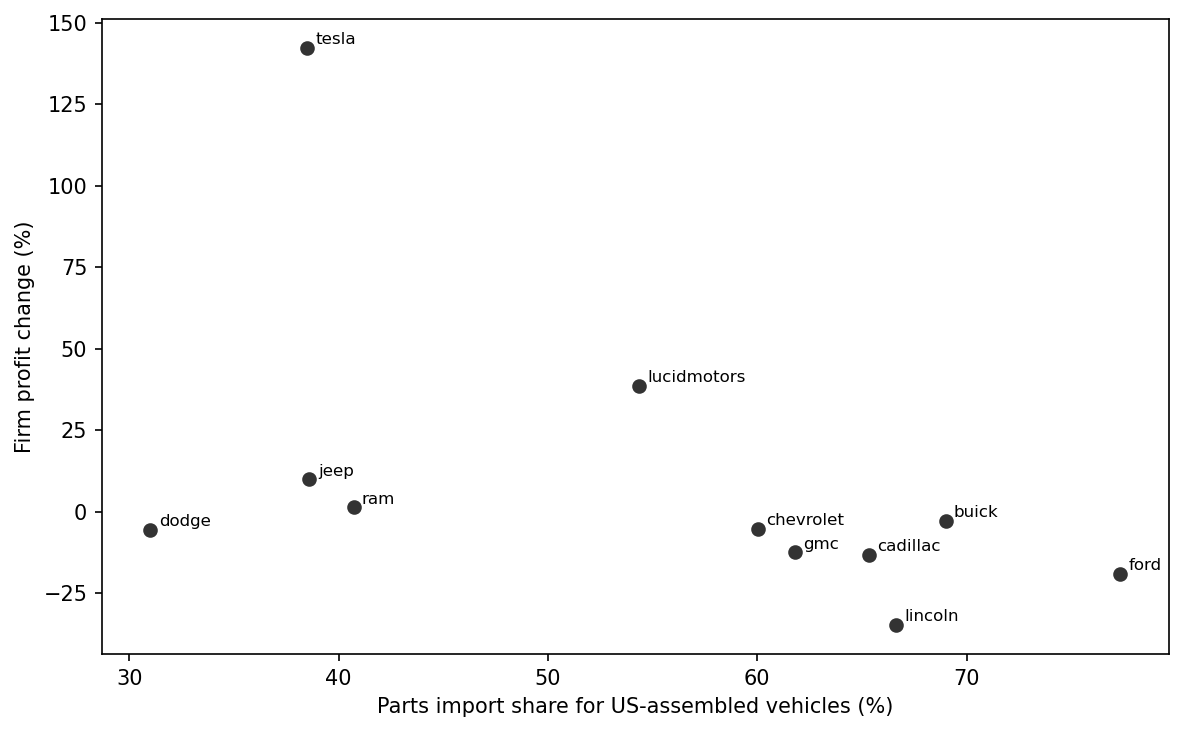
\includegraphics[width=1\linewidth]{generated/graphs/profit_change_vs_import_share_parts_and_vehicles_tariff__with_subsidy.png}
    \caption{US firms' profit change and parts import share: parts and vehicles tariffs, EV subsidy reinstated}
    \label{fig:profit_change_vs_import_share}
    \captionsetup{font=footnotesize, justification=raggedright, singlelinecheck=false}
    \caption*{\textit{Notes:} Only US-headquartered firms are show. Profit change in \% is compared to the 'no-tariffs, EV subsidy repealed' baseline. The x-axis is the sales-weighted share of parts imported for the US-assembled vehicles of each US-headquartered firm. The y-axis is the total profit change for the firm (including from any vehicles assembled abroad). Rivian has been removed from this chart as its import share \% was imputed as the average of all vehicles.}
\end{figure}

\begin{figure}[!htbp]
\centering
\begin{subfigure}[t]{0.8\linewidth}
    \centering
    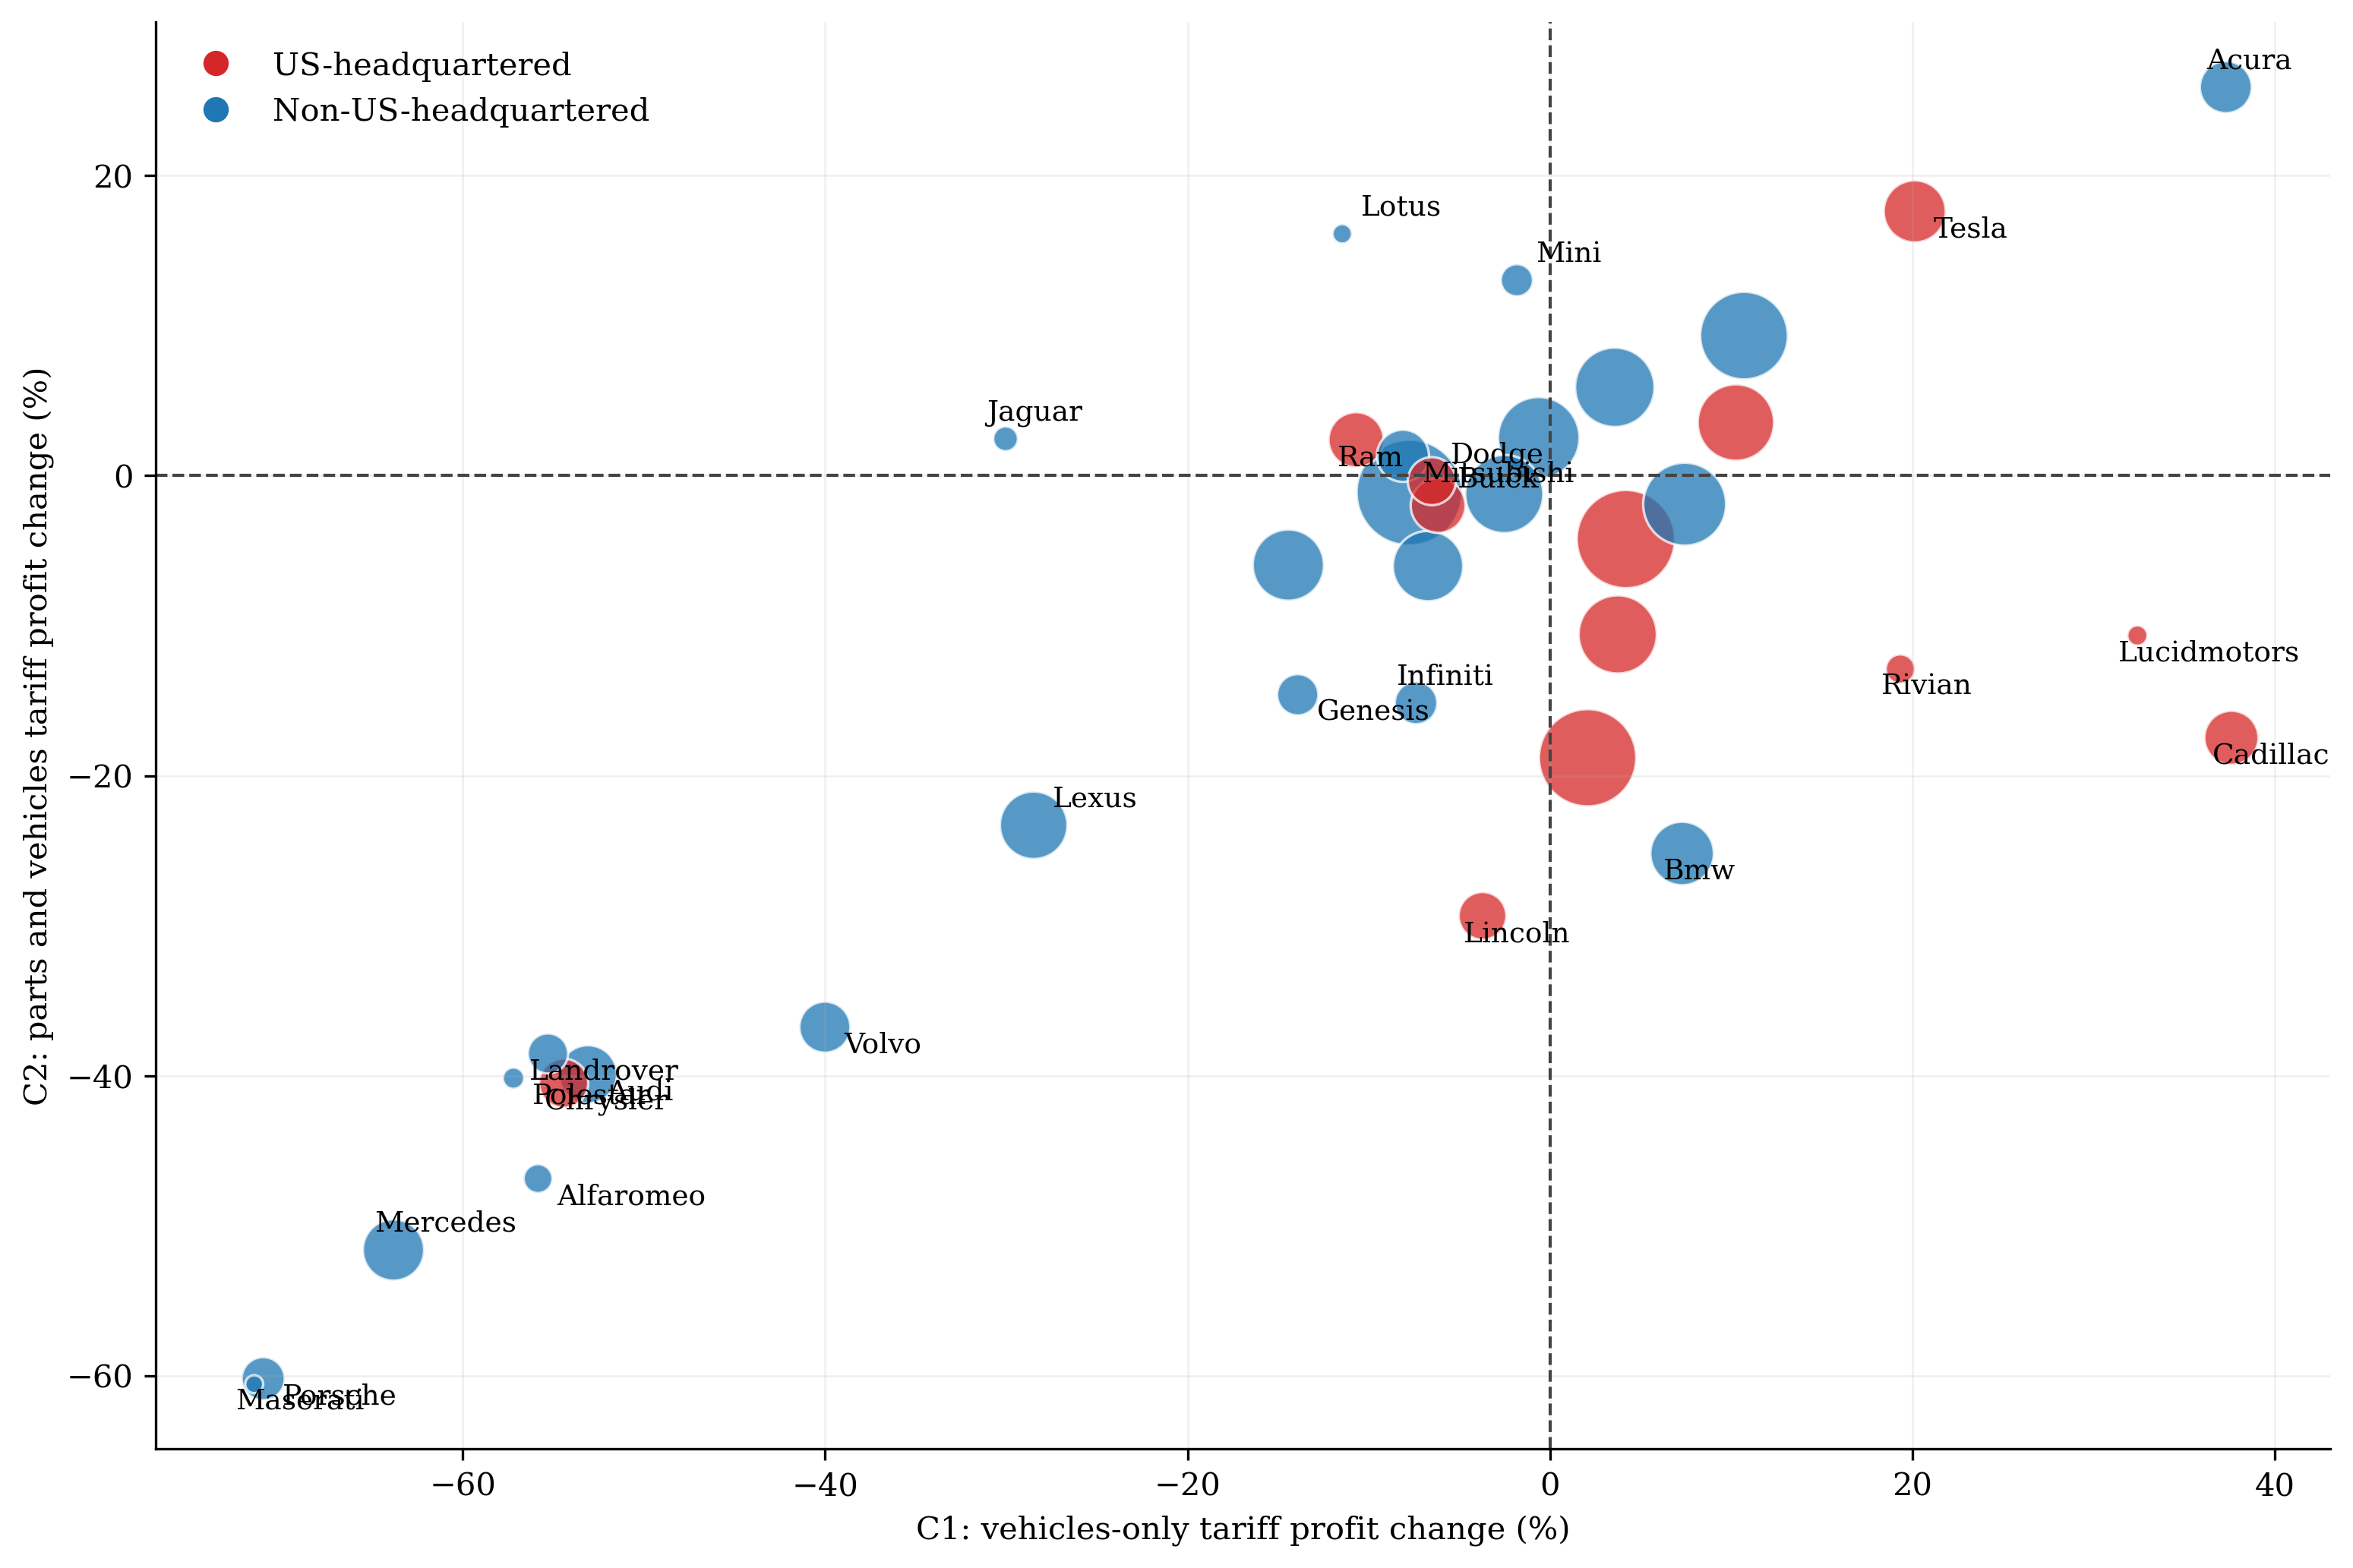
\includegraphics[width=\linewidth]{generated/graphs/z_scatter_pct_less.png}
    \caption{\textbf{Percentage profit changes across firms under tariff counterfactuals (remaining labels)}}
\label{fig:ps_scatter_pct_less}
\end{subfigure}\hfill%
\begin{subfigure}[t]{0.8\linewidth}
    \centering
    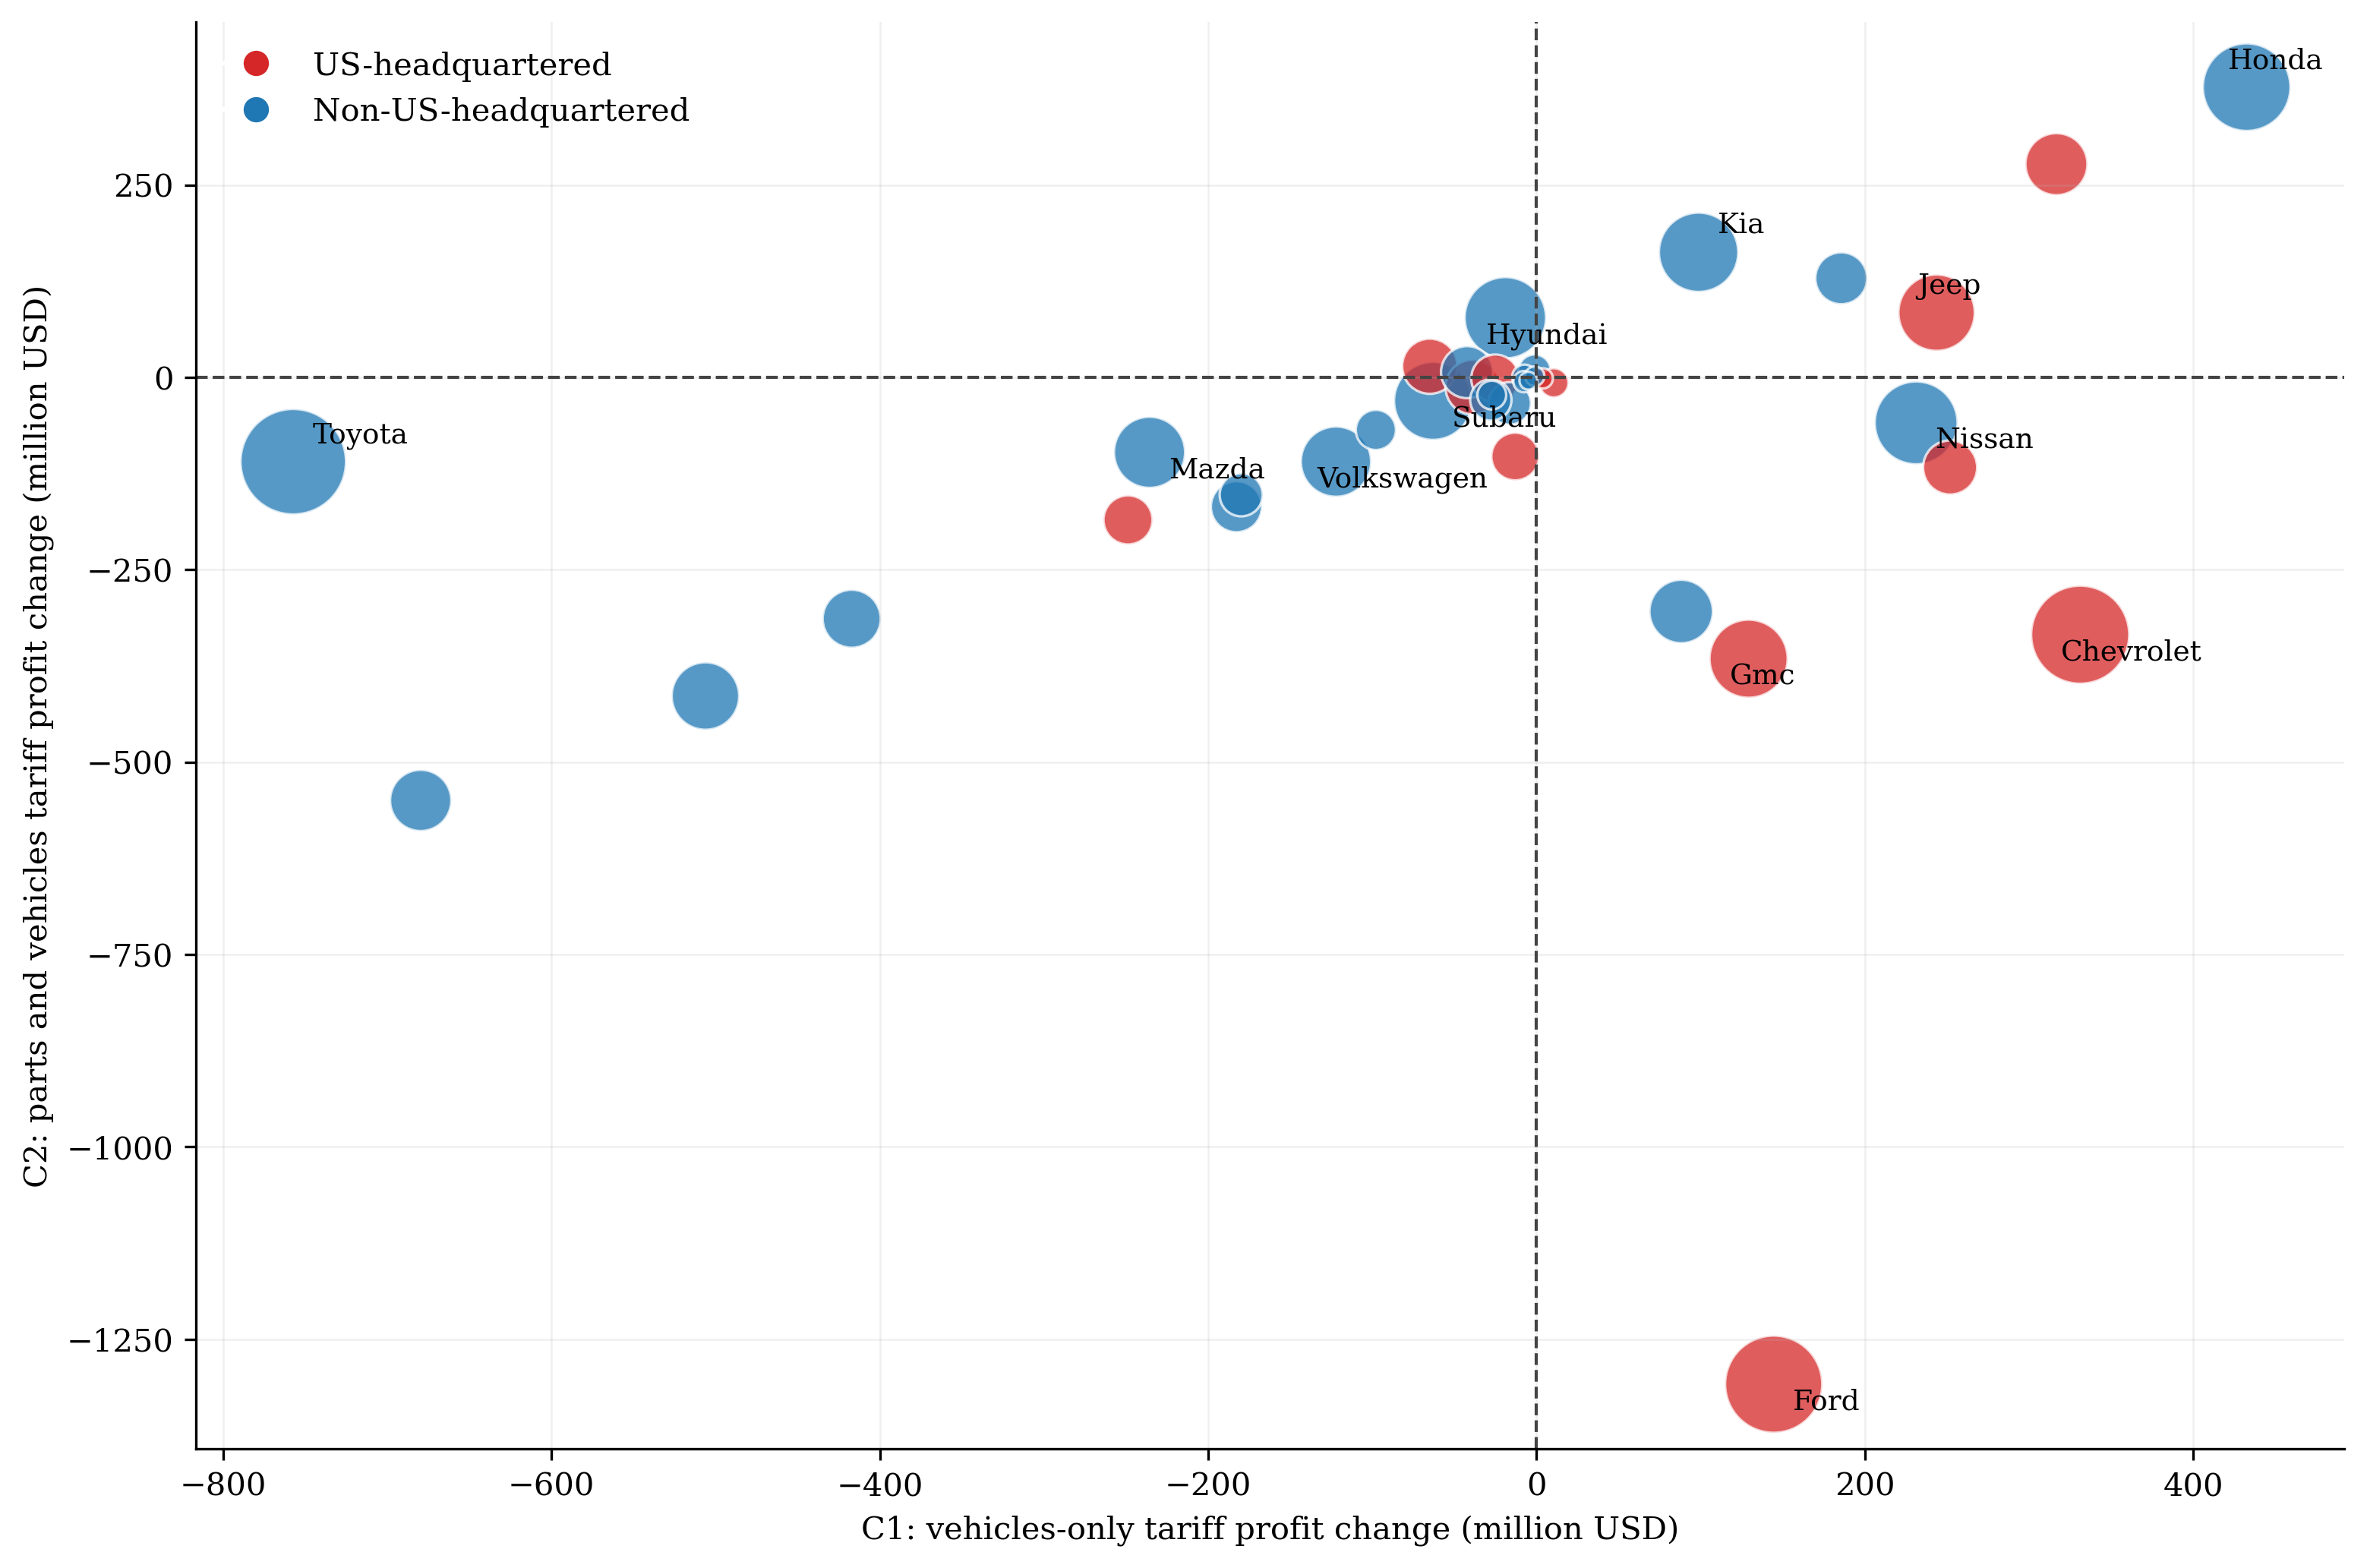
\includegraphics[width=\linewidth]{generated/graphs/z_scatter_usd_more.png}
    \caption{\textbf{Profit (USD) changes across firms under tariff counterfactuals}}
\label{fig:ps_scatter_usd_more}
\end{subfigure}
\caption{Changes by assembly-location: Tariff counterfactuals}
%\label{fig:origin_metrics_tariffs_no_subsidy}
\captionsetup{font=footnotesize, justification=raggedright, singlelinecheck=false}
\caption*{\textit{Notes:} These figures plot changes in firm-level profits relative to the baseline under two counterfactual tariff scenarios: C1 (25\% tariff on imported finished vehicles only) on the x-axis and C2 (25\% tariff applied to both imported vehicles and imported parts) on the y-axis.
Panel (a) reports the firm-level percentage profits changes with the label of the firms with less market share (labels missing in the Figure \ref{fig:ps_scatter_pct_more}). Panel (b) reports the change in profits in USD. }
\end{figure}

\setcounter{table}{0}
\renewcommand{\thetable}{B\arabic{table}}
\begin{table}[htbp]
\centering
\caption{Summary Statistics by Vehicle Type}
\label{tab:summary_by_type}
\footnotesize
\setlength{\tabcolsep}{6pt}
\renewcommand{\arraystretch}{1.15}
\begin{adjustbox}{max width=\textwidth}
\begin{tabular}{llllll}
\toprule
 &  & Cars, $N = 4178$ & Trucks, $N = 455$ & SUVs, $N = 3015$ & Vans, $N = 403$ \\
\midrule
\multirow{4}{*}{Sales} & Mean & 15,686 & 57,234 & 22,869 & 19,918 \\
  & Std. dev. & 33,280 & 92,476 & 38,741 & 25,606 \\
  & Min & 15 & 38 & 18 & 18 \\
  & Max & 334,818 & 529,238 & 374,263 & 130,780 \\
\midrule
\multirow{4}{*}{Price (2015 USD, \$100,000)} & Mean & 0.36 & 0.35 & 0.43 & 0.31 \\
  & Std. dev. & 0.17 & 0.07 & 0.16 & 0.05 \\
  & Min & 0.13 & 0.19 & 0.18 & 0.21 \\
  & Max & 1.00 & 0.74 & 1.00 & 0.47 \\
\midrule
\multirow{4}{*}{Horsepower (100s)} & Mean & 2.46 & 3.41 & 2.91 & 2.65 \\
  & Std. dev. & 1.04 & 0.97 & 0.89 & 0.64 \\
  & Min & 0.70 & 1.91 & 1.38 & 1.31 \\
  & Max & 8.45 & 8.35 & 8.35 & 4.01 \\
\midrule
\multirow{4}{*}{Footprint (square ft, 100s)} & Mean & 0.97 & 1.31 & 1.06 & 1.27 \\
  & Std. dev. & 0.12 & 0.19 & 0.12 & 0.20 \\
  & Min & 0.45 & 1.02 & 0.81 & 0.86 \\
  & Max & 1.27 & 1.84 & 1.40 & 1.92 \\
\midrule
\multirow{4}{*}{Curb weight (pounds, 1000s)} & Mean & 3.54 & 5.06 & 4.43 & 4.57 \\
  & Std. dev. & 0.57 & 0.87 & 0.76 & 0.64 \\
  & Min & 1.81 & 3.52 & 3.02 & 3.25 \\
  & Max & 5.92 & 9.10 & 6.92 & 5.99 \\
\midrule
\multirow{1}{*}{Imported (\%)} & Mean & 0.75 & 0.08 & 0.55 & 0.59 \\
\midrule
\multirow{1}{*}{Electric (\%)} & Mean & 0.06 & 0.04 & 0.05 & 0.00 \\
\bottomrule
\end{tabular}
\end{adjustbox}
\end{table}


\begin{figure}[!htbp]
\centering
\begin{adjustbox}{center}
    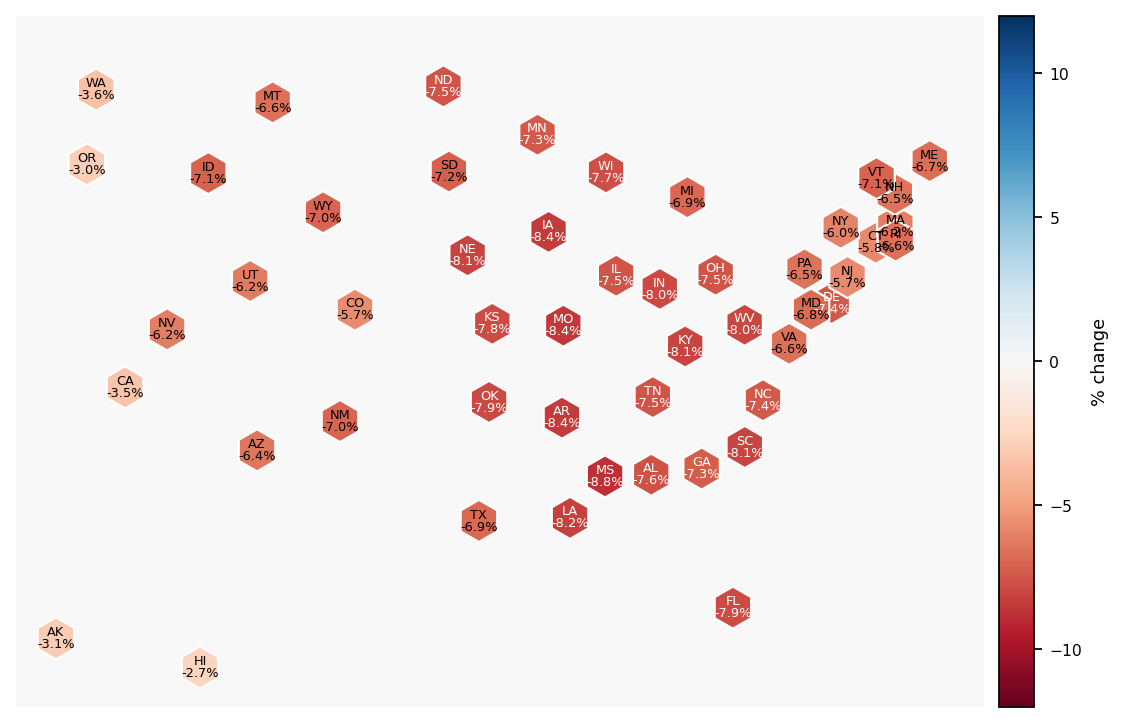
\includegraphics[width=.8\linewidth]{generated/graphs/cs_map_parts_and_vehicles_tariff__with_subsidy.png}
\end{adjustbox}
\caption{State consumer surplus impacts: parts and vehicles tariffs, EV subsidy reinstated}
\label{fig:cs_map_parts_and_vehicles_tariff__with_subsidy}
\captionsetup{font=footnotesize, justification=raggedright, singlelinecheck=false}
\caption*{\textit{Notes:} Consumer surplus change is relative to the 'no-tariffs, EV subsidy repealed' baseline. Labels for Rhode Island and Delaware have been removed.}
\end{figure}

\begin{figure}[!htbp]
    \centering
    % ---------------- Panel A ----------------
    \begin{subfigure}{1\linewidth}
        \centering
        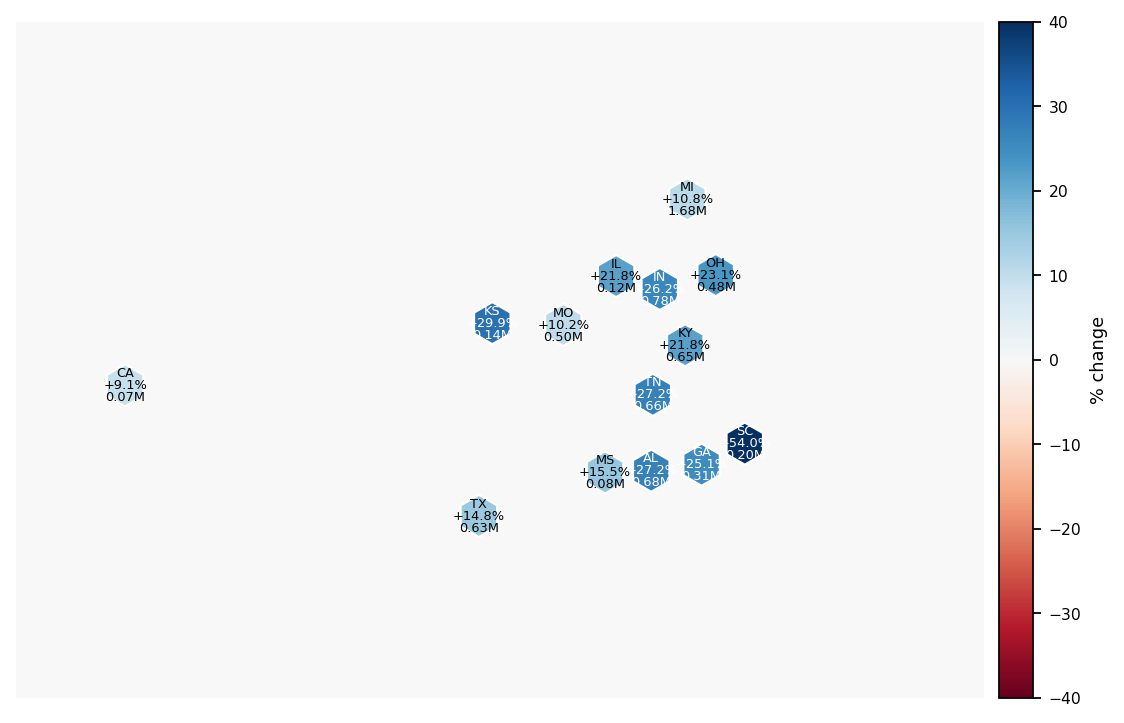
\includegraphics[width=1\linewidth]{generated/graphs/assembly_map_vehicles_only_tariff__no_subsidy.png}
        \caption{State assembly impacts: Vehicle-only tariff (C1)}
        \label{fig:assembly_map_vehicles_only_tariff__no_subsidy}
    \end{subfigure}
%    \vspace{0.6em}
    % ---------------- Panel B ----------------
    \begin{subfigure}{1\linewidth}
        \centering
        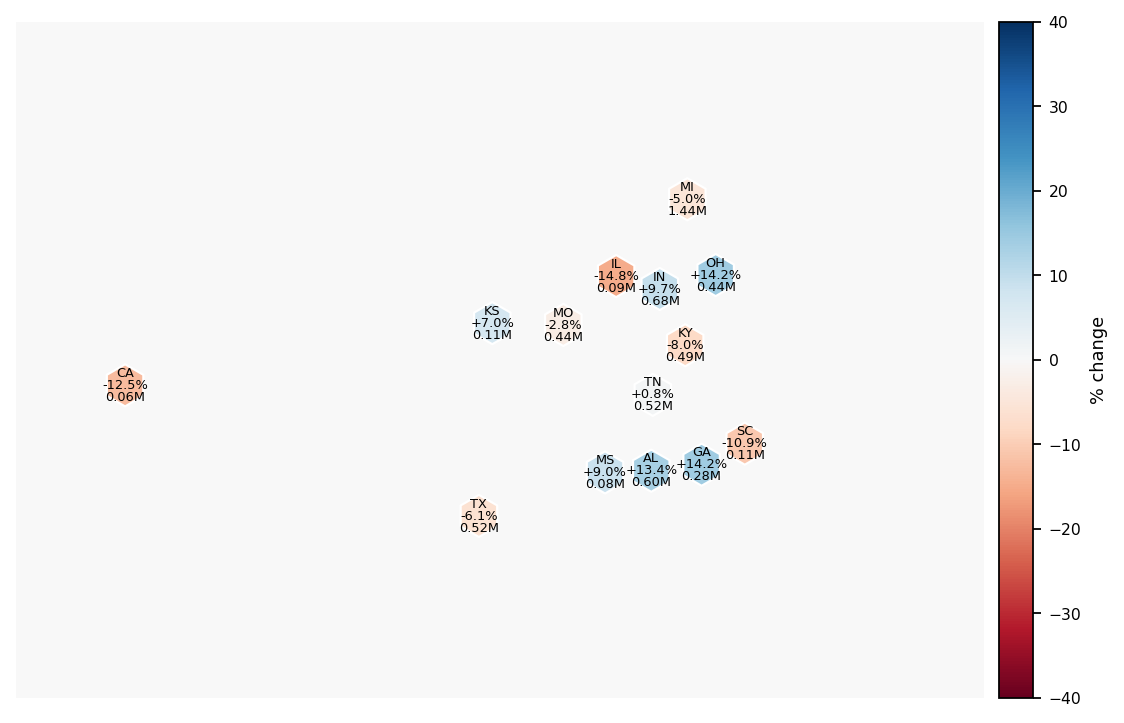
\includegraphics[width=1\linewidth]{generated/graphs/assembly_map_parts_and_vehicles_tariff__no_subsidy.png}
        \caption{State assembly impacts: Vehicle and parts tariffs (C2) }
        \label{fig:assembly_map_parts_and_vehicles_tariff__no_subsidy}
    \end{subfigure}
\caption{State assembly impacts: Tariff counterfactuals}
    \label{fig:assembly_map_tariffs_no_subsidy}
    \captionsetup{font=footnotesize, justification=raggedright, singlelinecheck=false}
    \caption*{\textit{Notes:} Values shown are total counterfactual vehicle production and \% change from 'no-tariffs, EV subsidy repealed' baseline. Arizona production has been removed as only the Lucid Air, with a negligible share, is produced there.}
\end{figure}

\begin{figure}
    \centering
    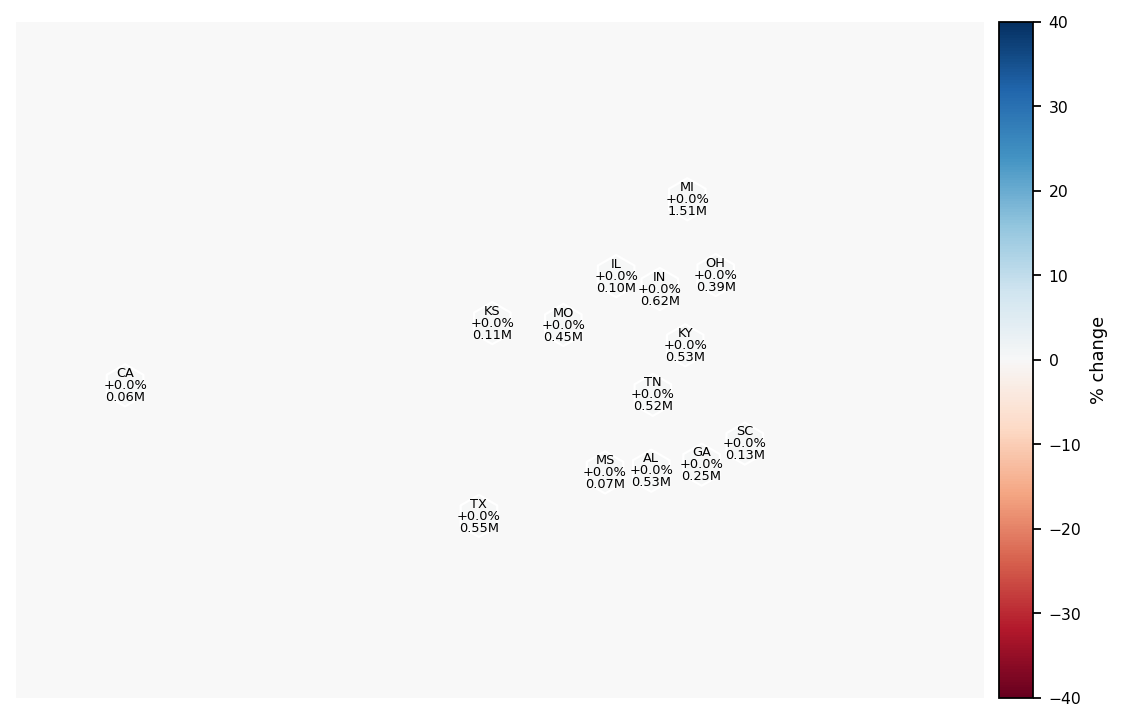
\includegraphics[width=1\linewidth]{generated/graphs/assembly_map_no_tariff__no_subsidy.png}
    \caption{State assembly impacts: No tariffs, subsidies removed.}
    \label{fig:assembly_map_no_tariff__no_subsidy}
    \captionsetup{font=footnotesize, justification=raggedright, singlelinecheck=false}
    \caption*{\textit{Notes:} Values shown are total counterfactual vehicle production and \% change from baseline. Arizona production has been removed as only the Lucid Air, with a negligible share, is produced there.}
\end{figure}

\clearpage
\section{Appendix Tables}\label{sec:appendix_table}

\input{generated/tables/avg_ev_subsidy_by_producer_45W}
%\input{Submission_draft/tables/avg_ev_subsidy_by_producer}

\begin{table}[!htbp]
\centering
\caption{Counterfactual Tariff and Subsidy Scenarios: 2024 Market Outcomes}
\label{tab:cf_summary_full}
\scriptsize
\setlength{\tabcolsep}{3pt}
\renewcommand{\arraystretch}{1.10}
\begin{adjustbox}{max width=\textwidth}
\begin{threeparttable}
\begin{tabular}{lcccccc}
\toprule
 & \multicolumn{3}{c}{Without Subsidy} & \multicolumn{3}{c}{With Subsidy} \\
\cmidrule(lr){2-4}\cmidrule(lr){5-7}
Tariff Status & B0: No & C1: Vehicles-only & C2: Parts \& vehicle & C3: No & C4: Vehicles-only & C5: Parts \& vehicle \\
\midrule
$\Delta$ Price (avg, \%) & 0.00 & 5.23 & 8.89 & -0.06 & 5.17 & 8.83 \\
Markup (avg \%) & 18.9 & 18.4 & 18.2 & 18.9 & 18.5 & 18.2 \\
$\Delta$ Markup (avg \%) & 0.0 & -0.5 & -0.7 & -0.0 & -0.5 & -0.7 \\
$\Delta$ US Producer Surplus (b USD) & 0.00 & 1.04 & -2.06 & 1.80 & 3.09 & -0.10 \\
CS $\Delta$ total (b USD) & 0.000 (0.0\%) & -14.116 (-4.3\%) & -29.793 (-9.1\%) & 10.055 (3.1\%) & -5.026 (-1.5\%) & -21.207 (-6.5\%) \\
CS $\Delta$ Q1 (b USD) & 0.000 (0.0\%) & -0.512 (-6.8\%) & -1.089 (-14.5\%) & 0.053 (0.7\%) & -0.471 (-6.3\%) & -1.065 (-14.2\%) \\
CS $\Delta$ Q2 (b USD) & 0.000 (0.0\%) & -1.540 (-5.6\%) & -3.161 (-11.5\%) & 0.746 (2.7\%) & -0.861 (-3.1\%) & -2.585 (-9.4\%) \\
CS $\Delta$ Q3 (b USD) & 0.000 (0.0\%) & -2.659 (-6.1\%) & -5.673 (-13.0\%) & 1.797 (4.1\%) & -1.076 (-2.5\%) & -4.293 (-9.8\%) \\
CS $\Delta$ Q4 (b USD) & 0.000 (0.0\%) & -3.629 (-5.0\%) & -7.686 (-10.6\%) & 2.981 (4.1\%) & -1.022 (-1.4\%) & -5.264 (-7.2\%) \\
CS $\Delta$ Q5 (b USD) & 0.000 (0.0\%) & -5.775 (-3.3\%) & -12.184 (-6.9\%) & 4.477 (2.5\%) & -1.596 (-0.9\%) & -8.000 (-4.5\%) \\
$\Delta$ vehicles sold (m) & 0.000 & -0.381 & -0.792 & 0.201 & -0.193 & -0.612 \\
EV share (\% sales) & 3.36 & 3.22 & 3.20 & 7.39 & 6.87 & 6.80 \\
US-assembled share (\% sales) & 53.2 & 65.9 & 57.7 & 53.5 & 66.2 & 58.2 \\
$\Delta$ US assembled (m) & 0.000 & 1.170 & 0.049 & 0.144 & 1.331 & 0.201 \\
Tariff revenue (b USD) & 0.000 & 14.55 & 40.29 & 0.000 & 14.79 & 40.88 \\
EV subsidy cost (b USD) & 0.000 & 0.000 & 0.000 & 6.68 & 6.11 & 5.75 \\
$\Delta$ Net US outcomes (b USD) & 0.00 & 1.48 & 8.44 & 5.17 & 6.75 & 13.83 \\
\bottomrule
\end{tabular}
\begin{tablenotes}[flushleft]\footnotesize
\item \textit{Notes:} $\Delta$ entries report counterfactual outcomes relative to the `no tariff, EV subsidy repealed' baseline. Dollars are USD 2015. $\Delta$ Net US outcomes is the change in US producer and consumer surplus, plus tariff revenue, minus (plus) additional EV subsidy expenditure (savings) compared to baseline. US Producer Surplus counts profit changes for US-headquartered firms. Consumer surplus (CS) changes are in billion USD; parentheses report percentage changes. `EV subsidy reinstated' and `EV subsidy repealed' refer to whether the EV subsidy policy is in place in the counterfactual.
\end{tablenotes}
\end{threeparttable}
\end{adjustbox}
\end{table}


\clearpage
\setcounter{table}{0}
\renewcommand{\thetable}{C\arabic{table}}
\section{Cost-Side Robustness}\label{sec:appendix_cost_side_robustness}

This appendix reports robustness checks for the imported-parts cost channel.

\subsection{Timing Diagnostics}

Tables \ref{tab:cost_reg_placebo_levels} and \ref{tab:cost_reg_placebo_fd} report robustness checks with respect to timing of the exchange rate shock. The first column in each table repeats the contemporaneous \(RER_t\) specification. The second column replaces the contemporaneous exchange rate with \(RER_{t+1}\). The third column includes the contemporaneous and one-year-ahead terms jointly. The fourth column reports the foreign-assembled placebo using the same exposure construction.

The timing checks show that the one-year-ahead exchange-rate term is positive. In levels, the \(RER_{t+1}\) term remains large when entered jointly with \(RER_t\), while the contemporaneous term falls close to zero. In first differences, the future term is still positive, though the contemporaneous term is more similar in magnitude. Table \ref{tab:cost_reg_timing_triplet_levels} and Table \ref{tab:cost_reg_timing_triplet_fd} add lagged exchange-rate terms to the timing diagnostic. Column (2) includes lagged, contemporaneous, and one-year-ahead terms; column (3) includes only lagged and contemporaneous terms. The comparison shows how much of the contemporaneous coefficient is recovered when the lagged term is included without conditioning on the future term.


\begin{table}[htbp]
   \caption{\label{tab:cost_reg_placebo_levels} Exchange-rate placebo regressions (levels)}
   \centering
   \begin{tabular}{lcccc}
      \tabularnewline \midrule \midrule
      Dependent Variable: & \multicolumn{4}{c}{ln\_costs}\\
       & \multicolumn{3}{c}{Domestic sample} & Foreign placebo \\
      Model:                                   & (1)            & (2)            & (3)            & (4)\\
      \midrule
      \emph{Variables}\\
      $\ln(\text{size})$                       & 0.5452$^{***}$ & 0.5037$^{***}$ & 0.5036$^{***}$ & -0.1112\\
                                               & (0.2007)       & (0.1905)       & (0.1909)       & (0.1976)\\
      $\ln(\text{weight})$                     & 0.3021$^{*}$   & 0.3843$^{**}$  & 0.3844$^{**}$  & 0.3867$^{**}$\\
                                               & (0.1749)       & (0.1597)       & (0.1620)       & (0.1549)\\
      $\ln(\text{hp})$                         & 0.1890$^{**}$  & 0.1957$^{**}$  & 0.1957$^{**}$  & 0.2554$^{***}$\\
                                               & (0.0825)       & (0.0780)       & (0.0787)       & (0.0532)\\
      $\ln(\text{mpg})$                        & -0.0945        & -0.0657        & -0.0657        & -0.0930\\
                                               & (0.0758)       & (0.0779)       & (0.0777)       & (0.0651)\\
      $\rho_{j,t-1}\times\log(RER_{jt})$       & 0.5980$^{**}$  &                & -0.0011        & -0.0495\\
                                               & (0.2292)       &                & (0.2137)       & (0.0772)\\
      $\rho_{j,t-1}\times\log(RER_{j,t+1})$    &                & 0.7390$^{***}$ & 0.7398$^{***}$ &   \\
                                               &                & (0.2222)       & (0.2180)       &   \\
      \midrule
      \emph{Fixed-effects}\\
      make\_model                              & Yes            & Yes            & Yes            & Yes\\
      year                                     & Yes            & Yes            & Yes            & Yes\\
      \midrule
      \emph{Fit statistics}\\
      Observations                             & 374            & 374            & 374            & 882\\
      R$^2$                                    & 0.97850        & 0.97929        & 0.97929        & 0.99152\\
      Within R$^2$                             & 0.18083        & 0.21088        & 0.21088        & 0.18728\\
      \midrule \midrule
      \multicolumn{5}{l}{\emph{Clustered (make\_model) standard-errors in parentheses}}\\
      \multicolumn{5}{l}{\emph{Signif. Codes: ***: 0.01, **: 0.05, *: 0.1}}\\
   \end{tabular}
\vspace{0.25em}
\begin{minipage}{0.96\textwidth}
\footnotesize \textit{Notes:} The dependent variable is log recovered marginal cost. Columns (1)--(3) use U.S.-assembled vehicles: column (1) includes the contemporaneous exchange-rate exposure term, column (2) replaces it with the one-year-ahead term, and column (3) includes both terms. Column (4) is a foreign-assembled placebo estimated with the contemporaneous exposure term on a different sample; it tests whether the same exposure construction predicts costs where the domestic imported-parts channel should not apply. All specifications include make-model and year fixed effects and vehicle controls. Standard errors are clustered by make-model.
\end{minipage}
\end{table}


\clearpage


\begin{table}[htbp]
   \caption{\label{tab:cost_reg_placebo_fd} Exchange-rate placebo regressions (first differences)}
   \centering
   \begin{tabular}{lcccc}
      \tabularnewline \midrule \midrule
      Dependent Variable: & \multicolumn{4}{c}{ln\_costs}\\
       & \multicolumn{3}{c}{Domestic sample} & Foreign placebo \\
      Model:                                          & (1)            & (2)            & (3)            & (4)\\
      \midrule
      \emph{Variables}\\
      $\Delta\ln(\text{size})$                        & 0.5088$^{*}$  & 0.5373$^{**}$  & 0.5250$^{**}$ & -0.0119\\
                                                      & (0.2569)      & (0.2563)       & (0.2550)      & (0.1926)\\
      $\Delta\ln(\text{weight})$                      & 0.4020$^{*}$  & 0.4201$^{*}$   & 0.4077$^{*}$  & 0.2900$^{**}$\\
                                                      & (0.2222)      & (0.2225)       & (0.2231)      & (0.1303)\\
      $\Delta\ln(\text{hp})$                          & 0.2137$^{**}$ & 0.2065$^{**}$  & 0.2061$^{**}$ & 0.2855$^{***}$\\
                                                      & (0.0998)      & (0.0968)       & (0.0978)      & (0.0569)\\
      $\Delta\ln(\text{mpg})$                         & -0.0448       & -0.0565        & -0.0559       & -0.1342$^{*}$\\
                                                      & (0.0692)      & (0.0758)       & (0.0742)      & (0.0787)\\
      $\rho_{j,t-1}\times\Delta\log(RER_{jt})$        & 0.4452$^{**}$ &                & 0.2133        & -0.0457\\
                                                      & (0.2136)      &                & (0.2329)      & (0.0805)\\
      $\rho_{j,t-1}\times\Delta\log(RER_{j,t+1})$     &               & 0.5756$^{***}$ & 0.4958$^{**}$ &   \\
                                                      &               & (0.2120)       & (0.2286)      &   \\
      \midrule
      \emph{Fixed-effects}\\
      year                                            & Yes           & Yes            & Yes           & Yes\\
      \midrule
      \emph{Fit statistics}\\
      Observations                                    & 255           & 255            & 255           & 590\\
      R$^2$                                           & 0.14428       & 0.15335        & 0.15492       & 0.32981\\
      Within R$^2$                                    & 0.11390       & 0.12329        & 0.12492       & 0.23399\\
      \midrule \midrule
      \multicolumn{5}{l}{\emph{Clustered (make\_model) standard-errors in parentheses}}\\
      \multicolumn{5}{l}{\emph{Signif. Codes: ***: 0.01, **: 0.05, *: 0.1}}\\
   \end{tabular}
\vspace{0.25em}
\begin{minipage}{0.96\textwidth}
\footnotesize \textit{Notes:} The dependent variable is the first difference of log recovered marginal cost. Columns (1)--(3) use U.S.-assembled vehicles observed in consecutive years: column (1) includes the contemporaneous exchange-rate exposure term, column (2) replaces it with the one-year-ahead exchange-rate difference, and column (3) includes both terms. Column (4) is a foreign-assembled placebo estimated on a different first-difference sample. All specifications include year fixed effects and differenced vehicle controls. Standard errors are clustered by make-model.
\end{minipage}
\end{table}


\clearpage


\begin{table}[htbp]
   \caption{\label{tab:cost_reg_timing_triplet_levels} Current, future, and lagged exchange-rate timing regressions (levels)}
   \centering
   \begin{tabular}{lccc}
      \tabularnewline \midrule \midrule
      Dependent Variable: & \multicolumn{3}{c}{ln\_costs}\\
                                               & Current + future & Lag + current + future & Lag + current \\
      Model:                                   & (1)            & (2)            & (3)\\
      \midrule
      \emph{Variables}\\
      $\ln(\text{size})$                       & 0.5036$^{***}$   & 0.4989$^{**}$          & 0.5184$^{**}$\\
                                               & (0.1909)         & (0.1932)               & (0.1999)\\
      $\ln(\text{weight})$                     & 0.3844$^{**}$    & 0.3710$^{**}$          & 0.3112$^{*}$\\
                                               & (0.1620)         & (0.1633)               & (0.1708)\\
      $\ln(\text{hp})$                         & 0.1957$^{**}$    & 0.1999$^{**}$          & 0.1999$^{**}$\\
                                               & (0.0787)         & (0.0788)               & (0.0807)\\
      $\ln(\text{mpg})$                        & -0.0657          & -0.0675                & -0.0858\\
                                               & (0.0777)         & (0.0765)               & (0.0741)\\
      $\rho_{j,t-1}\times\log(RER_{jt})$       & -0.0011          & 0.4083                 & 1.136$^{***}$\\
                                               & (0.2137)         & (0.2980)               & (0.3313)\\
      $\rho_{j,t-1}\times\log(RER_{j,t+1})$    & 0.7398$^{***}$   & 0.5773$^{***}$         &   \\
                                               & (0.2180)         & (0.2084)               &   \\
      $\rho_{j,t-1}\times\log(RER_{j,t-1})$    &                  & -0.4182                & -0.8094$^{***}$\\
                                               &                  & (0.3048)               & (0.3008)\\
      \midrule
      \emph{Fixed-effects}\\
      make\_model                              & Yes              & Yes                    & Yes\\
      year                                     & Yes              & Yes                    & Yes\\
      \midrule
      \emph{Fit statistics}\\
      Observations                             & 374              & 374                    & 374\\
      R$^2$                                    & 0.97929          & 0.97940                & 0.97904\\
      Within R$^2$                             & 0.21088          & 0.21494                & 0.20146\\
      \midrule \midrule
      \multicolumn{4}{l}{\emph{Clustered (make\_model) standard-errors in parentheses}}\\
      \multicolumn{4}{l}{\emph{Signif. Codes: ***: 0.01, **: 0.05, *: 0.1}}\\
   \end{tabular}
\vspace{0.25em}
\begin{minipage}{0.96\textwidth}
\footnotesize \textit{Notes:} The dependent variable is log recovered marginal cost. All columns use the same levels timing sample with non-missing lagged, contemporaneous, and one-year-ahead source-country exchange rates. Column (1) includes contemporaneous and one-year-ahead exposure terms. Column (2) adds the lagged exposure term. Column (3) includes lagged and contemporaneous exposure terms and excludes the one-year-ahead term. All specifications include make-model and year fixed effects and vehicle controls. Standard errors are clustered by make-model.
\end{minipage}
\end{table}


\clearpage


\begin{table}[htbp]
   \caption{\label{tab:cost_reg_timing_triplet_fd} Current, future, and lagged exchange-rate timing regressions (first differences)}
   \centering
   \begin{tabular}{lccc}
      \tabularnewline \midrule \midrule
      Dependent Variable: & \multicolumn{3}{c}{ln\_costs}\\
                                                      & Current + future & Lag + current + future & Lag + current \\
      Model:                                          & (1)            & (2)            & (3)\\
      \midrule
      \emph{Variables}\\
      $\Delta\ln(\text{size})$                        & 0.5250$^{**}$    & 0.4973$^{*}$           & 0.4843$^{*}$\\
                                                      & (0.2550)         & (0.2773)               & (0.2806)\\
      $\Delta\ln(\text{weight})$                      & 0.4077$^{*}$     & 0.3723                 & 0.3645\\
                                                      & (0.2231)         & (0.2265)               & (0.2252)\\
      $\Delta\ln(\text{hp})$                          & 0.2061$^{**}$    & 0.2166$^{**}$          & 0.2224$^{**}$\\
                                                      & (0.0978)         & (0.0944)               & (0.0944)\\
      $\Delta\ln(\text{mpg})$                         & -0.0559          & -0.0462                & -0.0385\\
                                                      & (0.0742)         & (0.0713)               & (0.0680)\\
      $\rho_{j,t-1}\times\Delta\log(RER_{jt})$        & 0.2133           & 0.5872$^{**}$          & 0.7697$^{***}$\\
                                                      & (0.2329)         & (0.2590)               & (0.2474)\\
      $\rho_{j,t-1}\times\Delta\log(RER_{j,t+1})$     & 0.4958$^{**}$    & 0.3126                 &   \\
                                                      & (0.2286)         & (0.2237)               &   \\
      $\rho_{j,t-1}\times\Delta\log(RER_{j,t-1})$     &                  & -0.7855$^{*}$          & -0.8842$^{**}$\\
                                                      &                  & (0.3960)               & (0.3862)\\
      \midrule
      \emph{Fixed-effects}\\
      year                                            & Yes              & Yes                    & Yes\\
      \midrule
      \emph{Fit statistics}\\
      Observations                                    & 255              & 255                    & 255\\
      R$^2$                                           & 0.15492          & 0.17321                & 0.16929\\
      Within R$^2$                                    & 0.12492          & 0.14385                & 0.13979\\
      \midrule \midrule
      \multicolumn{4}{l}{\emph{Clustered (make\_model) standard-errors in parentheses}}\\
      \multicolumn{4}{l}{\emph{Signif. Codes: ***: 0.01, **: 0.05, *: 0.1}}\\
   \end{tabular}
\vspace{0.25em}
\begin{minipage}{0.96\textwidth}
\footnotesize \textit{Notes:} The dependent variable is the first difference of log recovered marginal cost. All columns use the same consecutive-year timing sample with non-missing lagged, contemporaneous, and one-year-ahead exchange-rate differences. Column (1) includes contemporaneous and one-year-ahead exposure terms. Column (2) adds the lagged exposure term. Column (3) includes lagged and contemporaneous exposure terms and excludes the one-year-ahead term. All specifications include year fixed effects and differenced vehicle controls. Standard errors are clustered by make-model.
\end{minipage}
\end{table}


\clearpage
\subsection{Interpreting the One-Year-Ahead Exchange-Rate Coefficient}

The positive \(RER_{t+1}\) coefficient limits the strongest possible interpretation of the cost-side regression. The estimates should not be read as isolating only unanticipated contemporaneous annual exchange-rate shocks. Instead, the evidence is more naturally interpreted as identifying medium-run exposure to persistent foreign input cost conditions.

There are several reasons why this interpretation is economically plausible in the automobile setting. First, real exchange rates are persistent, so \(RER_{t+1}\) can proxy the persistent component of the exchange-rate environment that firms observe or forecast when setting prices and negotiating input costs \citep{rogoff_purchasing_1996}. Second, when market share has future value, current prices can respond to expected future exchange-rate conditions rather than only to current exchange rates \citep{froot_klemperer_1989}. Third, the pass-through literature emphasizes that exchange-rate effects need not be contemporaneous because invoicing currency, nominal rigidities, local costs, and strategic markups generate dynamic and incomplete pass-through \citep{gopinath_currency_2010,burstein_gopinath_2014}. Finally, automobile production involves model-year pricing, supplier contracts, and procurement lags. These features make calendar-year timing an imperfect proxy for the relevant cost window.

This interpretation is also consistent with the policy counterfactuals. Tariffs on imported parts are not transitory spot exchange-rate shocks. They are policy wedges that firms are likely to treat as persistent, especially when they affect model-year production and supplier contracts. The timing diagnostics therefore narrow the interpretation of the exchange-rate evidence, but they do not invalidate the use of the estimated coefficient as a medium-run imported-parts cost pass-through parameter.

\subsection{Prices, Marginal Costs, and Markups}

The next set of checks asks whether the exchange-rate exposure term appears in recovered marginal costs, observed prices, or recovered markups. This distinction matters because a coefficient that loaded only on recovered markups would be less consistent with an imported-input cost channel. This decomposition follows the spirit of structural exchange-rate work in automobile markets, which separates price responses into cost and markup components \citep{goldberg_verboven_2001}.

Table \ref{tab:cost_reg_price_markup_decomp} shows that the contemporaneous exposure term is positive for recovered marginal costs and observed prices, while recovered markups move in the opposite direction. These results suggest that the exchange-rate exposure term is visible in prices and recovered costs, which is the pattern one would expect if foreign input costs affect vehicle marginal costs and pricing.


\begin{table}[htbp]
   \caption{\label{tab:cost_reg_price_markup_decomp} Baseline exchange-rate decomposition across recovered costs, prices, and markups}
   \centering
   \resizebox{\textwidth}{!}{%
   \begin{tabular}{lcccccc}
      \tabularnewline \midrule \midrule
      Dependent Variables: & ln\_costs & ln\_prices & ln\_markups & \multicolumn{3}{c}{y}\\
       & \multicolumn{3}{c}{Levels} & \multicolumn{3}{c}{First differences} \\
      Model:                    & (1)            & (2)            & (3)            & (4)            & (5)            & (6)\\
      \midrule
      \emph{Variables}\\
      $\ln(\text{size})$        & 0.5452$^{***}$ & 0.4176$^{**}$ & -0.5763$^{***}$ & 0.5088$^{*}$  & 0.4328$^{*}$  & -0.3552$^{*}$\\
                                & (0.2007)       & (0.1672)      & (0.1731)        & (0.2569)      & (0.2233)      & (0.1918)\\
      $\ln(\text{weight})$      & 0.3021$^{*}$   & 0.2432        & -0.3766$^{**}$  & 0.4020$^{*}$  & 0.3315        & -0.4175$^{**}$\\
                                & (0.1749)       & (0.1509)      & (0.1874)        & (0.2222)      & (0.2084)      & (0.2004)\\
      $\ln(\text{hp})$          & 0.1890$^{**}$  & 0.1611$^{**}$ & -0.1720$^{***}$ & 0.2137$^{**}$ & 0.1736$^{**}$ & -0.2575$^{***}$\\
                                & (0.0825)       & (0.0739)      & (0.0605)        & (0.0998)      & (0.0869)      & (0.0862)\\
      $\ln(\text{mpg})$         & -0.0945        & -0.0896       & 0.0670          & -0.0448       & -0.0631       & -0.0833\\
                                & (0.0758)       & (0.0629)      & (0.0740)        & (0.0692)      & (0.0571)      & (0.0815)\\
      Current RER exposure term & 0.5980$^{**}$  & 0.4829$^{**}$ & -0.3523         & 0.4452$^{**}$ & 0.3625$^{**}$ & -0.3121\\
                                & (0.2292)       & (0.1901)      & (0.2352)        & (0.2136)      & (0.1702)      & (0.2990)\\
      \midrule
      \emph{Fixed-effects}\\
      make\_model               & Yes            & Yes           & Yes             &               &               & \\
      year                      & Yes            & Yes           & Yes             & Yes           & Yes           & Yes\\
      \midrule
      \emph{Fit statistics}\\
      Observations              & 374            & 374           & 374             & 255           & 255           & 255\\
      R$^2$                     & 0.97850        & 0.97931       & 0.96766         & 0.14428       & 0.14463       & 0.15772\\
      Within R$^2$              & 0.18083        & 0.16751       & 0.17948         & 0.11390       & 0.10498       & 0.14781\\
      \midrule \midrule
      \multicolumn{7}{l}{\emph{Clustered (make\_model) standard-errors in parentheses}}\\
      \multicolumn{7}{l}{\emph{Signif. Codes: ***: 0.01, **: 0.05, *: 0.1}}\\
   \end{tabular}%
   }
\vspace{0.25em}
\begin{minipage}{0.96\textwidth}
\footnotesize \textit{Notes:} Columns (1)--(3) are levels regressions with make-model and year fixed effects; columns (4)--(6) are first-difference regressions with year fixed effects. The dependent variables are log recovered marginal cost, log observed price, and log recovered markup, respectively. The reported exchange-rate coefficient is the contemporaneous source-country exchange-rate term interacted with lagged imported-parts exposure. All regressions include the vehicle controls shown in the table. Standard errors are clustered by make-model.
\end{minipage}
\end{table}


\clearpage

\subsection{Negative-Control Checks}

Table \ref{tab:leave_one_country_out_report} reports leave-one-source-country-out estimates. The levels coefficient remains positive when dropping each of the main observed source countries; the first-difference estimates are generally positive but become near zero when Japan is omitted. This is useful because the identifying variation is not mechanically pinned down by a single country. The foreign-assembled placebo in Tables \ref{tab:cost_reg_placebo_levels} and \ref{tab:cost_reg_placebo_fd} is close to zero, which is reassuring for the interpretation that the main coefficient captures a cost channel specific to domestically assembled vehicles relying on imported parts.


\begin{table}[htbp]
\centering
\caption{Leave-one-country-out baseline pass-through regressions}
\label{tab:leave_one_country_out_report}
\begin{tabular}{lcccc}
\toprule
Omitted country & Levels coef. & Levels $N$ & FD coef. & FD $N$ \\
\midrule
Full sample & 0.598 (0.229) & 374 & 0.445 (0.214) & 255 \\
Mexico & 1.250 (0.496) & 199 & 1.117 (0.497) & 143 \\
Japan & 0.605 (0.512) & 227 & -0.027 (0.451) & 142 \\
Korea & 0.628 (0.229) & 341 & 0.490 (0.222) & 238 \\
Germany & 0.608 (0.224) & 357 & 0.459 (0.218) & 243 \\
Spain & 0.597 (0.229) & 372 & 0.435 (0.215) & 254 \\
\bottomrule
\end{tabular}
\vspace{0.25em}
\begin{minipage}{0.96\textwidth}
\footnotesize \textit{Notes:} Each row re-estimates the baseline contemporaneous exchange-rate pass-through regression after omitting observations whose primary source country is listed in the first column. The full-sample row imposes no country omission. The levels specification includes make-model and year fixed effects and vehicle controls. The first-difference specification uses consecutive-year differences and year fixed effects. Coefficients are reported with make-model clustered standard errors in parentheses.
\end{minipage}
\end{table}


\subsection{Summary}

The robustness checks support the imported-parts cost channel. The exposure term appears in observed prices and recovered costs rather than only in recovered markups, the foreign-assembled placebo is close to zero, and the estimates are not driven by a single source country. The main limitation is timing: one-year-ahead exchange rates also predict current recovered costs. [TODO: Write interpretation]

\clearpage
\section{Appendix Text}
\subsubsection{Construction of Moments}\label{sec:appendix_moments}
\paragraph{Income-dependent micro-moment construction}

We use the CEX Interview Survey micro-data to construct income-dependent automobile purchase moments (\cite{bureau_of_labor_statistics_public_2025}). The CEX micro-data reports monthly expenditure on new vehicles linked to household income, which we aggregate to the annual level to construct our observed income micro parts:

\[
\mathbf{E}_t[\text{price paid}_{it} | \text{income quintile}_{it}],
\]

\noindent where price paid is the sum of net new-vehicle expenditures in that calendar year before the receipt of any appropriate electric vehicle subsidy.

To build purchase probability micro-moments we define an annual purchase indicator for each consumer unit as $\mathbf{1}[\text{purchase}] = \mathbf{1}[{\text{new vehicle spend >  0}}]$ and define the micro parts, namely:

\[
\mathbf{E}_t[\mathbf{1}[\text{purchase}_{it}]| \text{income quintile}_{it}].
\]

Income quintiles are constructed from the FMLI annual income, using survey weights to form weighted quintile cutoffs within each year.

\paragraph{Division dependent micro-moments}

We construct division micro-moments by aggregating state-based sales to the division level. We define the probability of a household purchasing an electric vehicle, conditional on their associated division, as:

\[
P(EV | purchase, d, t) = \frac{\text{total EV sales}_{d,t}}{\text{total vehicle sales}_{d,t}},
\]

\noindent where $d$ denotes the division. Observed moments for Truck and SUV sales are computed analogously.

\end{document}



% old
\begin{figure}[!htbp]
\centering
\begin{subfigure}[t]{0.48\linewidth}
    \centering
    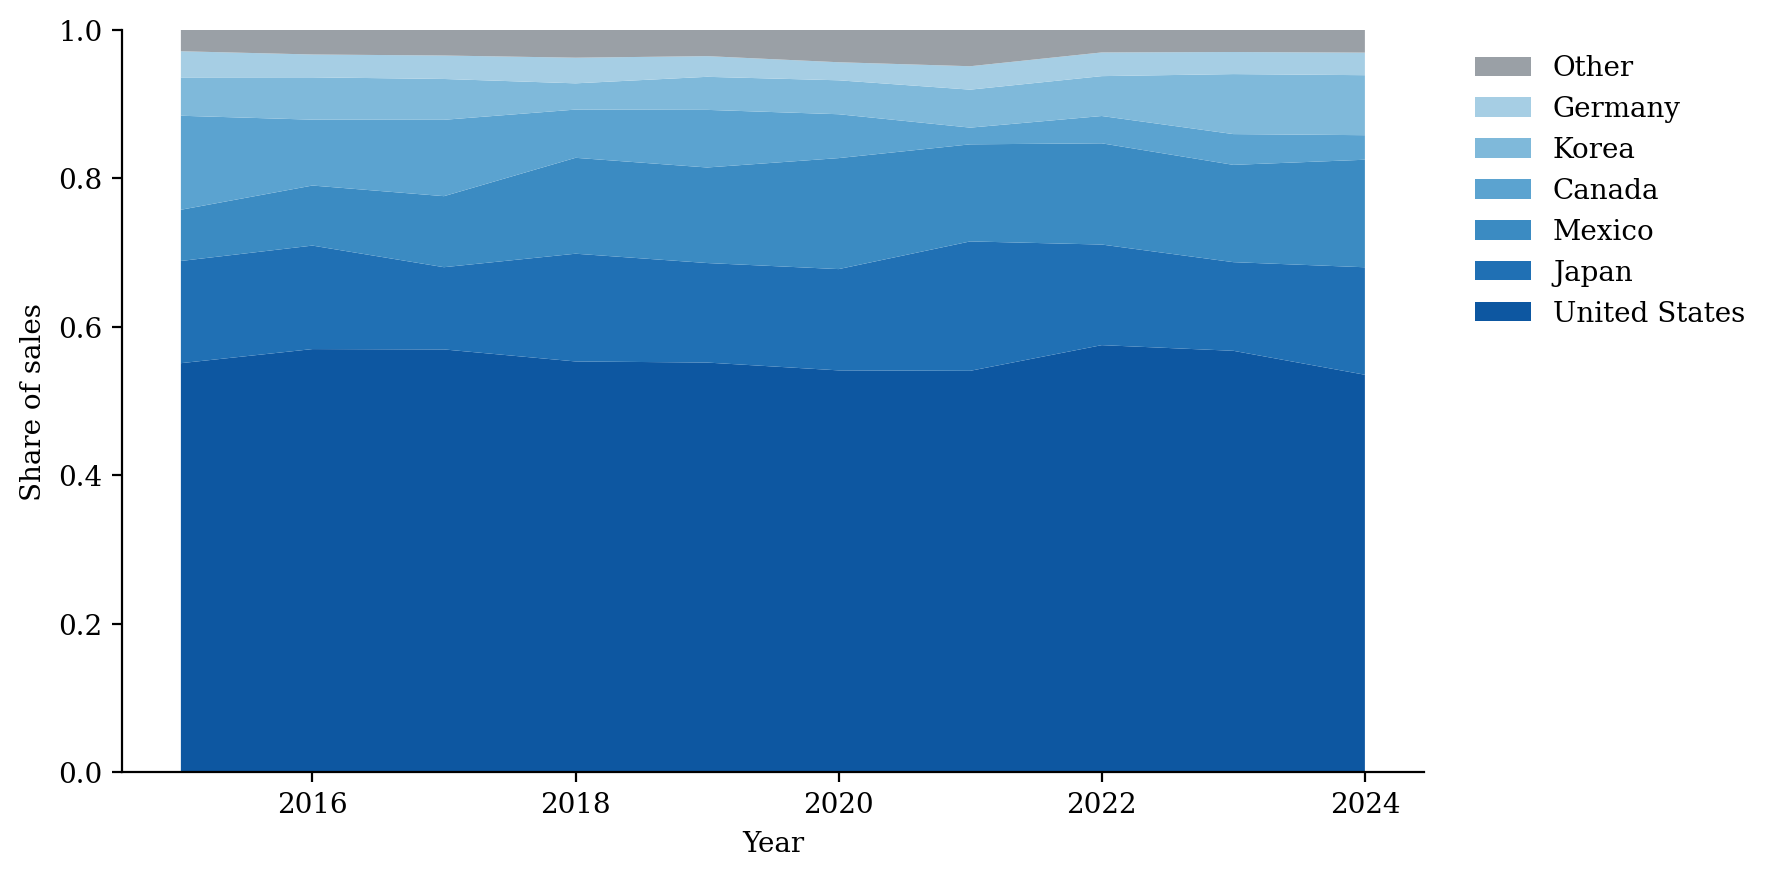
\includegraphics[width=\linewidth]{generated/graphs/sales_weighted_sources_by_year.png}
    \caption{{Assembly location of the vehicles sold in the United States}}
    \label{fig:sales_sources}
\end{subfigure}\hfill%
\begin{subfigure}[t]{0.48\linewidth}
    \centering
    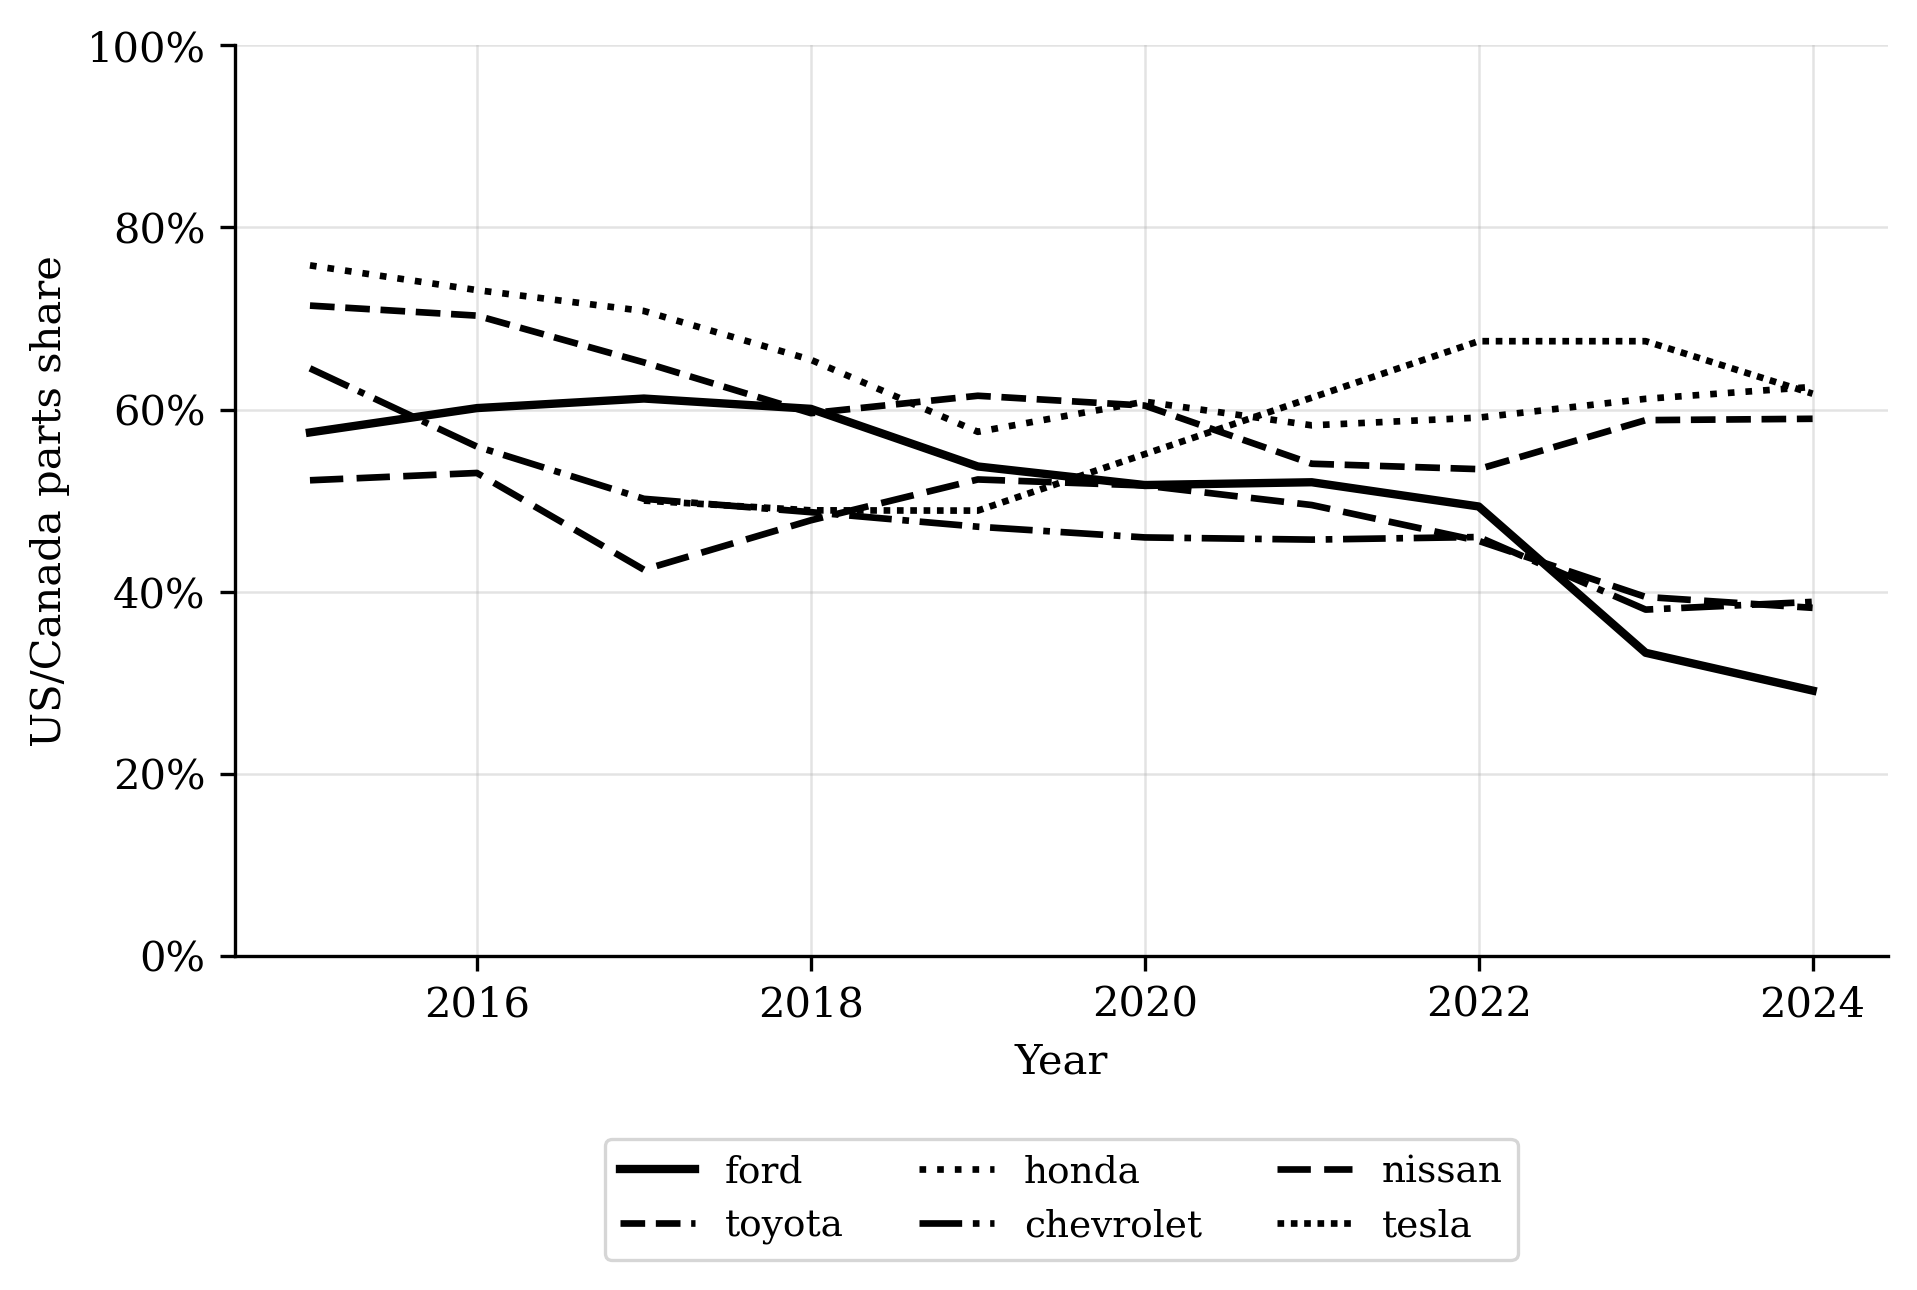
\includegraphics[width=\linewidth]{generated/graphs/domestic_share.png}
    \caption{{Share of US/CA parts in domestically assembled vehicles (by value)}}
    \label{fig:dom_share}
\end{subfigure}
\caption{Sources of vehicles sold and share of domestic production}
\label{fig:origin_metrics_tariffs_no_subsidy}
\end{figure}

\begin{figure}
    \centering
    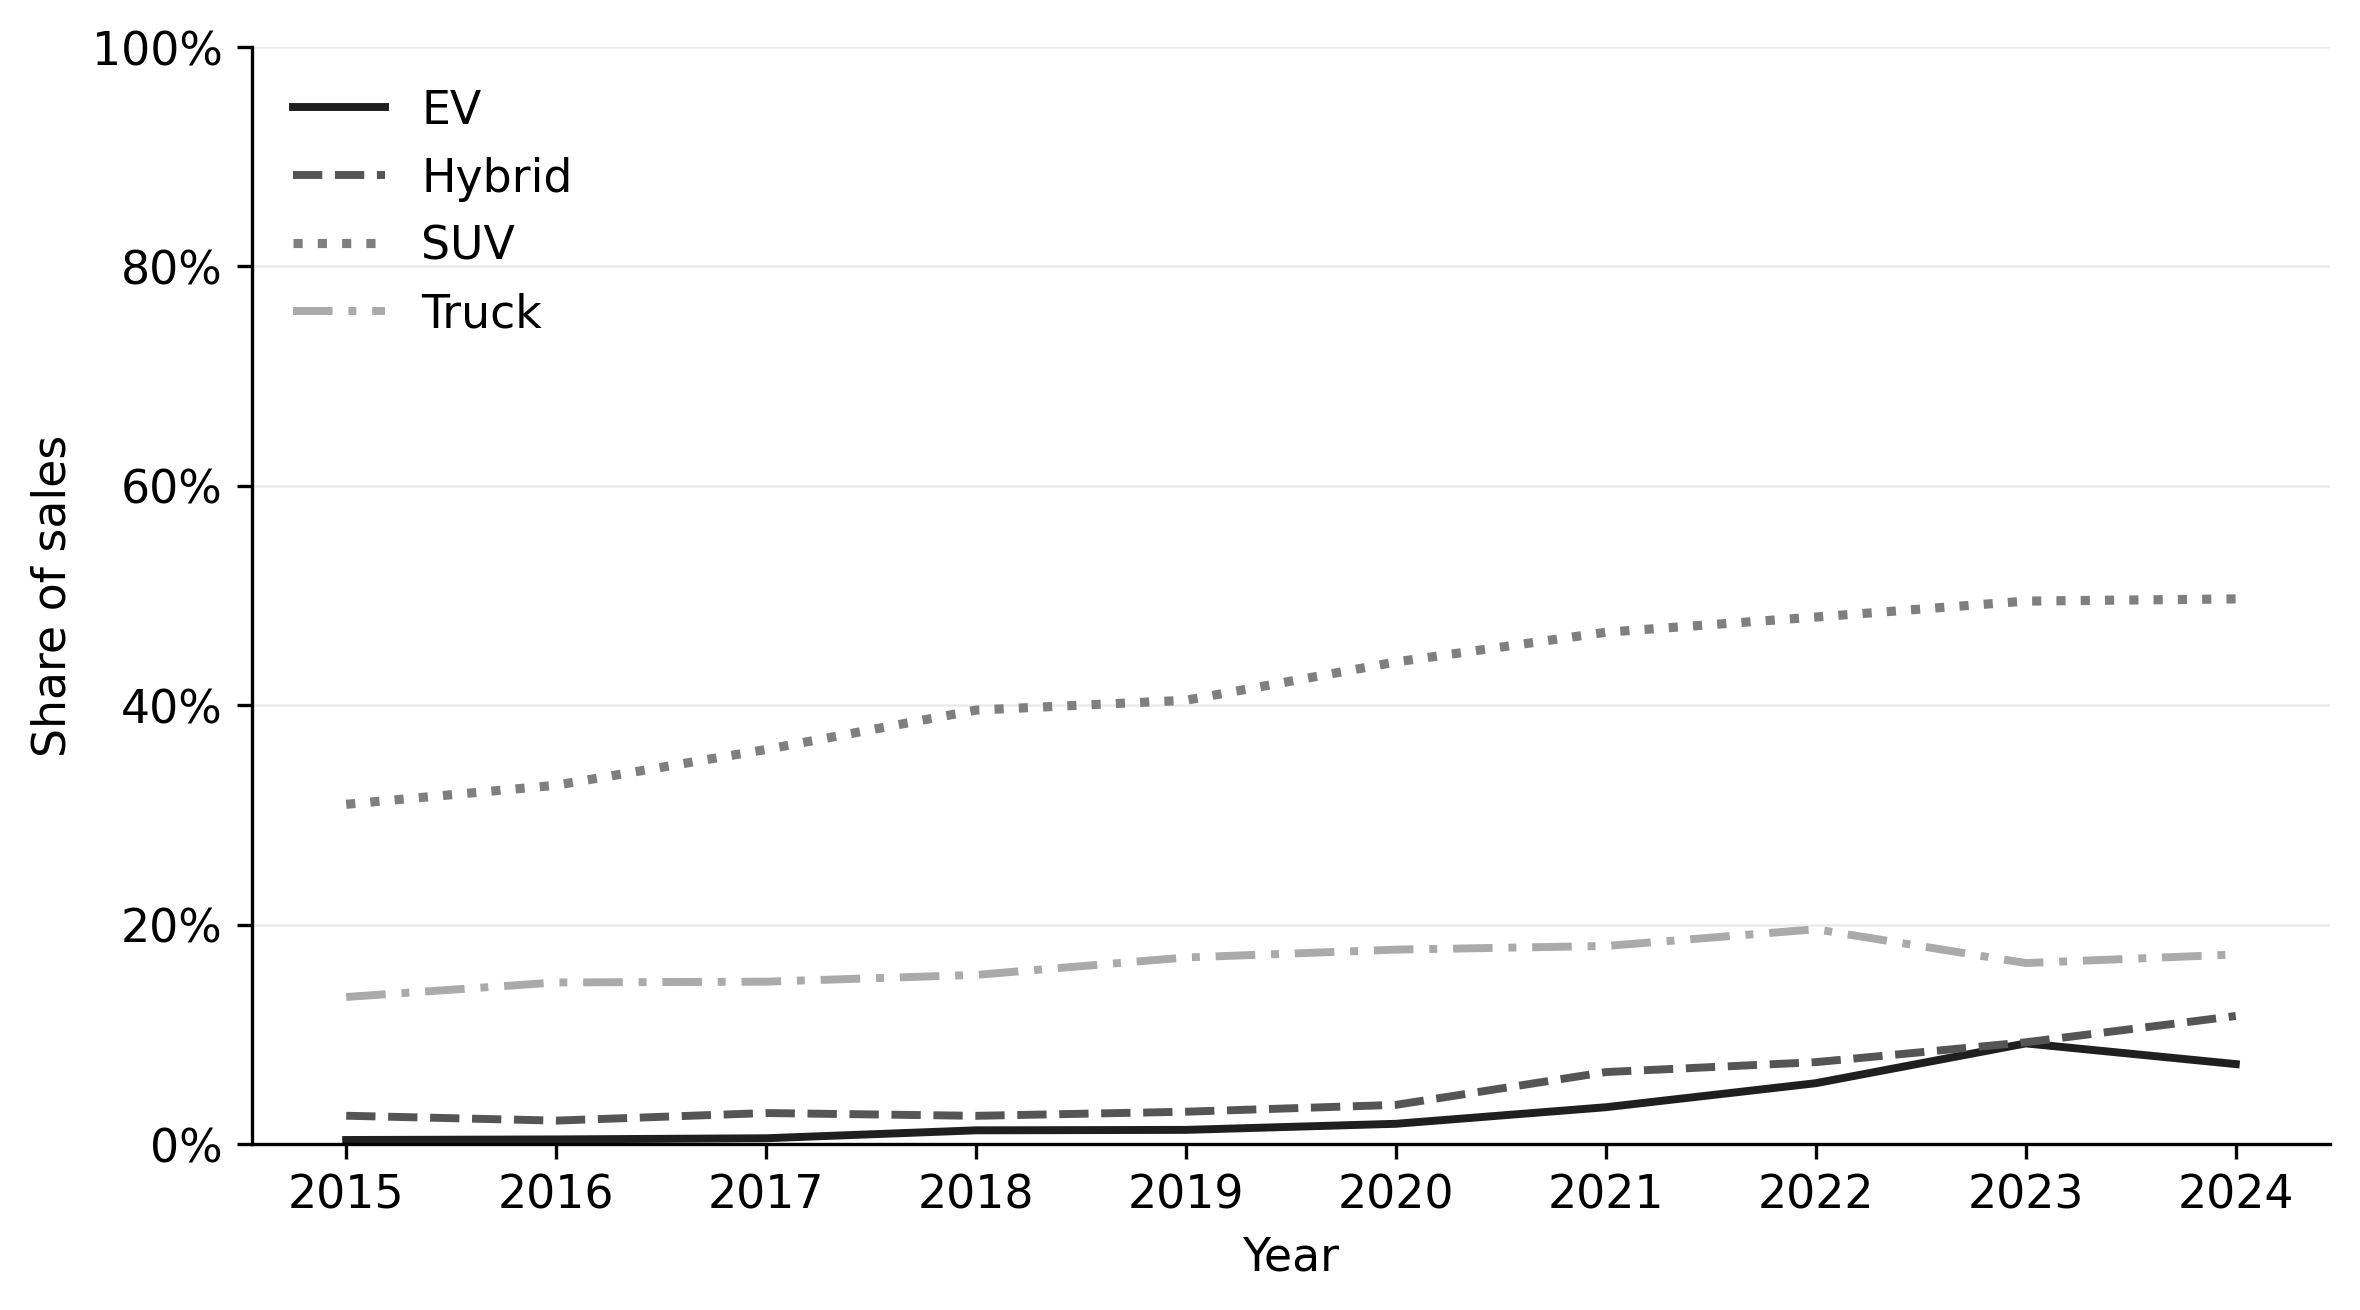
\includegraphics[width=0.8\linewidth]{generated/graphs/trends.png}
    \caption{Trends in sales by car type}
    \label{fig:trends}
\end{figure}
